%%%%%%%%%%%%%%%%%%%%%%%%%%%%%%%%%%%%%%%%%%%%%%%%%%%%%%%%%%%%%%%
\documentclass[12pt]{book}
\usepackage[a4paper,top=1.5in,bottom=1.5in,left=1in,right=1in]{geometry} 
\usepackage{fancyhdr}
\usepackage{fourier-orns}
\pagestyle{fancy}
\usepackage{graphicx}
\usepackage{lipsum} % for dummy text, you can remove this line in your actual document

\usepackage{amsmath, amssymb, bm}
\usepackage{caption}
\usepackage{graphicx} 
\usepackage[colorinlistoftodos]{todonotes}
\usepackage[colorlinks=true, allcolors=black]{hyperref}
\usepackage{float}
\usepackage{setspace}
% \usepackage{subfigure}
\usepackage{url}
\usepackage{tabularx}
\usepackage[utf8]{inputenc}
\usepackage{mathptmx} %Times Font
\usepackage{titlesec}
\titlespacing{\chapter}{0pt}{0pt}{0pt}
\usepackage{fancyhdr}
\usepackage{etoolbox}
\usepackage{appendix}
\usepackage{siunitx}
\usepackage{nomencl}
\newcommand{\nomunit}[1]{%
\renewcommand{\nomentryend}{\hspace*{\fill}#1}}
\makenomenclature%
\usepackage{caption}
\usepackage{lipsum}
\usepackage{algpseudocode}
\usepackage{empheq}
\usepackage{mdwlist}
\usepackage{booktabs}
\usepackage{colortbl}
\widowpenalty10000
\clubpenalty10000
\usepackage{moresize}
\usepackage{tabularray}
\usepackage[style=apa]{biblatex}
\usepackage{subcaption}
\usepackage{array}
\usepackage{adjustbox}

\addbibresource{References.bib}
\DeclareSourcemap{
  \maps[datatype=bibtex]{
    \map{
       \step[fieldsource=title, match=\regexp{\b([A-Z]{2,})\b}, replace={{}{$1}}]
    }
  }
}
 
\DeclareCaptionType{appfigure}[Figure]
\DeclareCaptionType{apptable}[Table]
\renewcommand{\listappfigurename}{List of Appendix Figures}
\renewcommand{\listapptablename}{List of Appendix Tables}
\renewcommand{\thefigure}{\thechapter-\arabic{figure}}
\renewcommand{\thetable}{\thechapter-\arabic{table}}
\renewcommand{\theappfigure}{\thechapter-\arabic{appfigure}}
\renewcommand{\theapptable}{\thechapter-\arabic{apptable}}
\renewcommand{\contentsname}{Table of Contents}
\renewcommand{\thefigure}{\arabic{figure}}
\renewcommand{\thetable}{\arabic{table}}

\newcommand{\chapname}{Chapter }
 
\titleformat{\chapter}[block]
{\bfseries\LARGE\centering}
{}{1em}{}[\rule{\textwidth}{0.3pt}]

\titleformat{\section}
{\bfseries\large}
{\thesection}{1em}{}

\titleformat{\subsection}
{\normalfont\bfseries}
{\thesubsection}{1em}{}

\titleformat{\subsubsection}
{\normalfont\bfseries}
{\thesubsubsection}{1em}{}

\usepackage{fancyhdr}
\usepackage{multirow}
\usepackage{multicol}

\usepackage{placeins}

\makeatletter
\renewcommand*\env@matrix[1][*\c@MaxMatrixColsc]{%
  \hskip -\arraycolsep%
  \let\@ifnextchar\new@ifnextchar%
  \array{#1}}
\makeatother

\usepackage{enumitem}

\usepackage{listings}
\usepackage{color}
 
\definecolor{codegreen}{rgb}{0,0.6,0}
\definecolor{codegray}{rgb}{0.5,0.5,0.5}
\definecolor{codepurple}{rgb}{0.58,0,0.82}
\definecolor{backcolour}{rgb}{0.95,0.95,0.95}

\newcommand{\codesize}{\fontsize{10pt}{11pt}\selectfont}

\lstdefinestyle{mystyle}{
    backgroundcolor=\color{backcolour},   
    commentstyle=\color{codegreen},
    keywordstyle=\color{magenta},
    numberstyle=\tiny\color{codegray},
    stringstyle=\color{codepurple},
    basicstyle=\ttfamily\codesize,
    breakatwhitespace=true,         
    breaklines=true,                 
    captionpos=b,                    
    keepspaces=false,                 
    numbers=left,                    
    numbersep=5pt,                  
    showspaces=false,                
    showstringspaces=false,
    showtabs=false,                  
    tabsize=2,
    showlines = true,
    fontadjust = true,
    framexleftmargin = 10 pt,
    resetmargins = true,
    basewidth = 0.5em
}
 
\lstset{style=mystyle}

\makeatletter
\setlength{\@fptop}{0pt}
\makeatother

\setlength{\floatsep}{0pt}

\newenvironment{Figure}
  {\noindent\minipage{\linewidth}}
  {\endminipage}

\setcounter{secnumdepth}{5}

\hyphenpenalty10000
\usepackage{multicol}
 
%%%%%%%%% MATHEMATICS SHORTHANDS %%%%%%%%%%%%%%%%%%%% 

\newcommand{\C}{\mathbb{C}}
\newcommand{\R}{\mathbb{R}}
\newcommand{\Z}{\mathbb{Z}}
\renewcommand{\d}{\mathrm{d}}
\renewcommand{\bf}[1]{\mathbf{#1}}

\newcommand{\argmax}[1]{\underset{#1}{\operatorname{arg\,max}}}

\newcommand{\kurt}{\mathrm{kurt}}
\newcommand{\round}{\operatorname{round}}

\newcommand{\E}{\operatorname{E}}
\newcommand{\cov}{\operatorname{cov}}
\newcommand{\pcov}{\operatorname{pcov}}

\newcommand*{\vertbar}{\rule[-1ex]{0.5pt}{2.5ex}}
\newcommand*{\horzbar}{\rule[.5ex]{2.5ex}{0.5pt}}

\setlength{\nomlabelwidth}{3cm}
\setlength{\nomitemsep}{-0.5\parsep}

\usepackage{makecell}
\usepackage{emptypage}

\newcolumntype{R}{>{\raggedleft\arraybackslash}X}
\newcolumntype{L}{>{\raggedright\arraybackslash}X}
\newcolumntype{C}{>{\centering\arraybackslash}X}

\usepackage{textcomp}
\usepackage{microtype}

\renewcommand{\headrule}{%
\vspace{-8pt}\hrulefill%
\raisebox{-2.1pt}{\quad\decofourleft\decotwo\decofourright\quad}\hrulefill}
\renewcommand{\sectionmark}[1]{\markright{#1}}



\sloppy
% \raggedright
\raggedbottom

% Set \headheight
\setlength{\headheight}{16.64995pt}

% Optionally adjust \topmargin
\addtolength{\topmargin}{-4.64995pt}

\usepackage{footmisc}

\usepackage{footnote}

\usepackage{tabularray}

\begin{document}

\renewcommand{\thesection}{\arabic{section}.} % Change section numbering style


\begin{titlepage}
\begin{figure}[!t]
\centering

\includegraphics[width = 4.2in]{Title/logo.png}
\caption*{}
\end{figure}

\centering
\LARGE{\textbf{PROJECT TITLE GOES HERE}}\\[1in]

\LARGE{\textbf{YOUR NAME}}\\
\normalsize{Matriculation number}\\[0.2in]

\large{Supervisor: XXXXX}\\
\large{Co-supervisor: XXXXX}\\[0.5in]

\large{A Final Year Report submitted to School of Physical and Mathematical Sciences, Nanyang Technological University in partial fulfilment of the requirements for the Degree of }\\[0.1in]

\Large{BACHELOR OF SCIENCE WITH HONOURS IN PHYSICS
}\\[1in]


\Large{2020/2021 Semester 1}
\newpage
\end{titlepage}

%=== FRONT PART ===
%=== ABSTRCT ===

%\begin{center}
\chapter*{Abstract} 
% \section{Abstract}
\rhead{Abstract}
%\end{center}
% \addcontentsline{toc}{chapter}{Abstract}
% Insert a horizontal line
% \rule{\textwidth}{0.4pt}
% \par\noindent\rule{\textwidth}{0.4pt}

% \vspace*{5mm}
%===============================
% ABSTRACT GOES HERE - 250 words limit
%===============================
Vivamus non vehicula tortor. Aenean tincidunt vel nisi id tincidunt. Aliquam eget sollicitudin ipsum. Curabitur quis malesuada magna. Integer nec condimentum sapien. Donec finibus rutrum tellus vel feugiat. Fusce auctor lectus id nunc dignissim, et ultricies eros volutpat. Pellentesque condimentum sed mi et placerat. Morbi semper, erat vitae sodales lobortis, orci enim viverra urna, et mollis mi dui ut ante. Vestibulum sodales lacinia scelerisque. Donec ut augue tellus. Etiam sit amet lacinia ipsum. Morbi commodo, sem sollicitudin dictum fringilla, libero quam varius erat, vel elementum felis velit ut elit. Fusce at sagittis eros. Phasellus tempor ullamcorper massa, consectetur scelerisque purus facilisis in. Vestibulum tempus eros vel sapien rutrum ullamcorper. Fusce at facilisis risus. Donec porttitor augue eu quam tempor, eget cursus risus commodo. Pellentesque sollicitudin, ipsum in tincidunt sagittis, nibh metus ultrices eros, egestas iaculis arcu justo non lectus. Praesent mollis orci ac sodales mollis. Sed suscipit sollicitudin ex id volutpat. Praesent laoreet molestie cursus. Nam dapibus dapibus bibendum. Donec maximus, velit non commodo porttitor, eros lacus ultrices ante, nec interdum purus mauris quis turpis. Nam dapibus quis lacus sed finibus. Aliquam venenatis, ex sit amet suscipit tempor, leo metus porta nulla, a egestas dui mi non risus. Duis vel libero ut mauris sodales cursus nec nec eros. Donec accumsan justo dolor. Quisque varius sem id dui dignissim, sed porta massa sodales. Nulla facilisi. Phasellus id metus ut enim eleifend volutpat. Fusce iaculis sodales tincidunt. Fusce quis convallis justo. Phasellus elementum, felis vel ultrices ultricies, ex nulla euismod justo, et.
%===============================
\\
\par
\textbf{Keywords:} Blind source separation, Independent component analysis, Independent vector analysis, Sparse component analysis, Automatic speech recognition, Android application development.

%=== END OF ABSTRACT ===

\newpage

%=== FRONT PART ===
%=== ACKNOWLEDGEMENT ===

%\begin{center}
\chapter*{Acknowledgement}
\rhead{Acknowledgement}
%\end{center}
\addcontentsline{toc}{chapter}{Acknowledgement}

Lorem ipsum dolor sit amet, consectetur adipiscing elit, sed do eiusmod tempor incididunt ut labore et dolore magna aliqua. Ut enim ad minim veniam, quis nostrud exercitation ullamco laboris nisi ut aliquip ex ea commodo consequat. Duis aute irure dolor in reprehenderit in voluptate velit esse cillum dolore eu fugiat nulla pariatur. Excepteur sint occaecat cupidatat non proident, sunt in culpa qui officia deserunt mollit anim id est laborum.


%=== END OF ACKNOWLEDGEMENT  ===

\newpage


%\include{Front/Nomenclature}
%\newpage

\renewcommand{\listfigurename}{Lists of Figures}
% \rhead{Lists of Figures}
\listoffigures 
\addcontentsline{toc}{chapter}{Lists of Figures}

\newpage


\listoftables 
\addcontentsline{toc}{chapter}{Lists of Tables}
% \rhead{Lists of Tables}
\newpage

\tableofcontents
\addcontentsline{toc}{chapter}{Table of Contents}
% \rhead{Table of Contents}
\newpage


% Set the page style to "fancy"...
\pagestyle{fancy}
%... then configure it.

% Clear all headers and footers (see also \fancyhf{})
\fancyhead{}\fancyfoot{}

% Set the header and footer for Even
% pages but omit the zone (L, C or R)
\fancyhead[R]{\nouppercase{\rightmark\hfill\leftmark}}
% \fancyhead[L]{\thepage} % Only show page number

% \fancyhead[R]{\hfill\thepage}
% \fancyhead[R]{\thepage} % Only show page number
\fancyfoot[L]{\rule{\textwidth}{0.4pt}\hspace{1cm} Intelligent Field Robotic Systems}
% \fancyfoot[R]{\rule{\textwidth}{0.4pt}\hspace{1cm} U6972746} % Add the line before the footer text
\fancyfoot[R]{\rule{\textwidth}{0.4pt}\hspace{1cm} \thepage} % Add the line before the footer text
% \fancyfoot[R]{\thepage} % Only show page number


% Some content:
% \renewcommand{\rightmark}{\thesection\ \leftmark} 









% Sections start from here  

\section{Introduction}

In recent years, the intersection of robotics and agriculture has garnered significant attention due to its potential to revolutionize farming practices and address various challenges in crop cultivation and management. One of the critical issues faced by farmers worldwide is the proliferation of weeds in agricultural fields, which not only compete with crops for essential resources but also pose significant threats to livestock health and food safety. In particular, weeds such as Rumex have been identified as major nuisances in grasslands, where their presence can contaminate forage intended for grazing animals, including cows.

\vspace*{6mm}

The purity of grassland vegetation directly impacts the nutritional quality of forage consumed by livestock, thereby influencing the health and productivity of animals. The ingestion of contaminated forage, tainted with toxic or harmful weed species like Rumex, can lead to adverse health effects in cattle, affecting milk quality and quantity, as well as overall animal welfare. Therefore, the effective removal of weeds, particularly Rumex, from grasslands is imperative to ensure the integrity and safety of livestock feed, as well as the sustainability of agricultural operations.

\vspace*{6mm} 


In response to this pressing agricultural challenge posed by weed infestation in grasslands, this thesis endeavors to pioneer the development and implementation of an innovative coverage path planning (CPP) algorithm. Unlike conventional approaches, this algorithm prioritizes straight paths to optimize energy efficiency, thereby offering versatility across a spectrum of coverage path planning methodologies. While its primary application lies in weed removal within grasslands, its adaptability extends to diverse agricultural contexts, promising enhanced efficiency and sustainability in autonomous robotic operations. CPP plays a crucial role in guiding autonomous robotic systems to systematically traverse and cover an entire area of interest while minimizing overlap and maximizing efficiency. By leveraging advancements in robotics, artificial intelligence, and sensing technologies, CPP algorithms can enable autonomous agricultural robots to navigate complex terrain, identify weed-infested areas, and perform targeted weed removal tasks with precision and efficacy.

\vspace*{6mm} 

The primary objective of this research is to develop a coverage path planning (CPP) algorithm tailored for the intelligent and systematic removal of Rumex weeds from grasslands, thereby promoting the production of high-quality forage and safeguarding the health of grazing animals. This algorithm aims to optimize coverage efficiency, ensuring that all targeted weeds are effectively identified and removed by the robotic system. Through the integration of advanced robotics algorithms, the proposed approach seeks to enhance the efficacy of weed management practices while minimizing reliance on chemical herbicides and manual labor.


\vspace*{6mm} 

This thesis will explore various aspects of coverage path planning (CPP) in the context of agricultural robotics, including but not limited to:
\begin{itemize}

  \item Review of Literature: A comprehensive overview of path planning techniques, including coverage path planning (CPP) and alternatives accommodating non-holonomic constraints. It explores classical and heuristic algorithms, their optimization strategies, and computational complexities, underscoring the importance of effective path planning in agricultural robotics. Through synthesizing diverse research streams, this review informs the development of an innovative CPP algorithm for weed removal.
  
  \item Methodology: We provide an in-depth exploration of the proposed CPP algorithm designed specifically for autonomous weed removal operations. We elucidate the underlying design principles governing the algorithm's development, emphasizing its adaptability to varying terrain and distinct dataset. Furthermore, we outline the computational framework, detailing the algorithm's implementation and optimization strategies to ensure efficient coverage and weed removal. Additionally, we discuss sensor integration strategies, elucidating how sensor data is utilized for perception and decision-making during weed removal tasks. Finally, we delve into the decision-making processes guiding the robotic system's actions, encompassing strategies for global and local path planning and obstacle avoidance to maximize efficiency and effectiveness in weed management operations.
  
  \item Experimental Setup: This section outlines the key considerations for field deployment and validation of the CPP algorithm in real-world grassland environments. It discusses the selection of robotic hardware, focusing on factors such as mobility, durability, and compatibility with the intended application. Additionally, it elaborates on the sensor configurations essential for environmental perception and obstacle detection during weed removal operations. The section also addresses field testing protocols, detailing the procedures for data collection, performance evaluation, and validation of the CPP algorithm's efficacy under actual operating conditions.
  
  \item Results and Analysis: This section presents a comprehensive analysis of experimental findings obtained through both simulation and real-world field trials, encompassing various parameters crucial for field robotics. It includes quantitative assessments of weed removal efficiency, coverage completeness, Energy usage, and to name a few. Furthermore, it compares the performance of the proposed CPP algorithm with other state-of-the-art approaches, considering factors such as path optimality, computational efficiency, and adaptability to different environments. Through a rigorous evaluation framework, this analysis provides valuable insights into the effectiveness and applicability of the CPP algorithm in practical agricultural settings.
  
  \item Discussion and Implications: This section engages in a thorough analysis of the research findings in the context of existing literature, elucidating the alignment and disparities between the proposed CPP algorithm and previous studies. It identifies the strengths and limitations of the algorithm, considering factors such as computational efficiency, scalability, and adaptability to diverse agricultural environments. Furthermore, it explores potential applications of the CPP algorithm beyond weed removal, highlighting its broader implications for sustainable agriculture and livestock management practices. By synthesizing empirical evidence with theoretical insights, this discussion offers valuable perspectives on the future trajectory of autonomous robotics in agriculture.

\end{itemize}

\vspace*{6mm} 


By addressing these key components, this thesis aims to contribute to the advancement of autonomous weed management technologies in the agricultural sector, with a specific focus on improving the health and productivity of grassland ecosystems and ensuring the safety and quality of livestock feed. Through interdisciplinary collaboration and innovative engineering solutions, the integration of CPP algorithms into agricultural robotics holds promise for mitigating weed-related challenges and fostering sustainable farming practices for the benefit of farmers, consumers, and the environment alike.

\vspace*{6mm} 


By meticulously addressing these critical components, this thesis endeavors to significantly propel the evolution of autonomous weed management technologies within the agricultural domain. With a targeted emphasis on enhancing the health and productivity of grassland ecosystems, as well as safeguarding the safety and quality of livestock feed, the research aims to effect tangible improvements across multiple facets of agricultural sustainability.

\vspace*{6mm} 

Through a concerted effort to foster interdisciplinary collaboration and devise innovative engineering solutions, the integration of Coverage Path Planning (CPP) algorithms into agricultural robotics emerges as a beacon of hope for mitigating the myriad challenges posed by weed infestation. This holistic approach not only promises to alleviate immediate concerns for farmers but also extends its benefits to end consumers and the environment at large.

\vspace*{6mm} 

By empowering farmers with efficient and effective weed management tools, the research seeks to enhance agricultural productivity while reducing reliance on conventional, often environmentally detrimental, weed control methods. Moreover, by promoting sustainable farming practices, the integration of CPP algorithms holds the potential to foster long-term environmental stewardship and contribute to the preservation of natural ecosystems.

\vspace*{6mm} 

Ultimately, the overarching goal of this thesis is to usher in a new era of agricultural innovation—one characterized by the harmonious coexistence of technological advancement and environmental conservation. By harnessing the power of robotics and leveraging the principles of sustainable agriculture, the research endeavors to create a brighter future for farmers, consumers, and the planet alike.

\vspace*{6mm} 

need to include the algorithm of the paper as did in the first review paper 

\newpage 

\chapter{Literature Review}
\section{Literature Review for CPP Algorithms.}


Path planning algorithms play a crucial role in the field of robotics and autonomous navigation, enabling vehicles to navigate efficiently through complex environments while adhering to various constraints. Coverage path Planning (CPP) is an open problem in robotics in improving the efficiency of planning an optimal path to cover the target area, as well as generating a collision-free pathway with less computation. An overview of CPP problems with the objective, challenges, and design features as mention in the paper \hyperlink{cite.main_review}{[2]} is shown in (\autoref{fig:overview_of_CPP})


\begin{figure}[htbp]
    \centering
    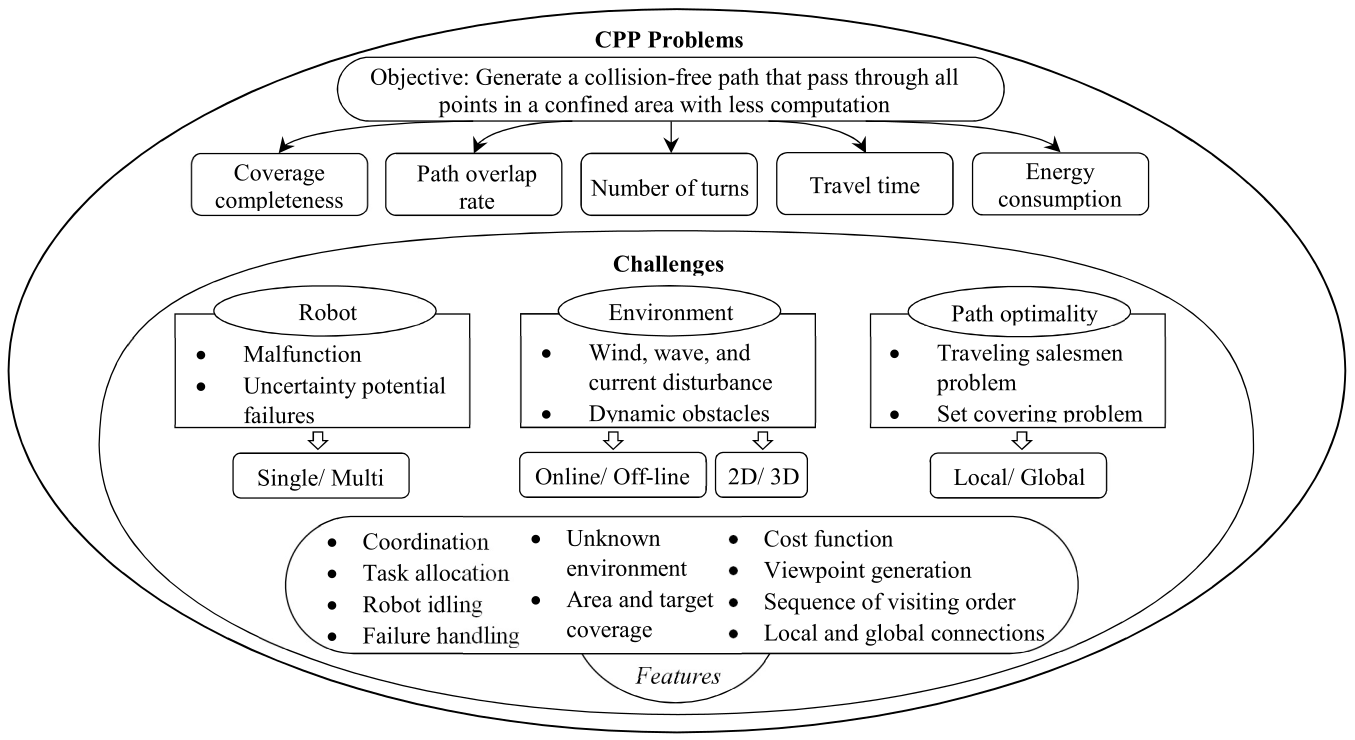
\includegraphics[width=\textwidth]{Images/general/overview_of_CPP.png}
    \caption{The objective and challenges in coverage path planning (CPP) problems.}
    \label{fig:overview_of_CPP}
\end{figure}

Over the years, researchers have developed a myriad of algorithms to address different aspects of path planning, ranging from basic algorithms to more advanced methodologies. CPP algorithms can be categorized into two approaches, classical algorithms, and heuristic-based algorithms. The summarized details of CPP algorithms according to the characteristics of the algorithms as stated in the paper \hyperlink{cite.main_review}{[2]} are classified as shown in (\autoref{fig:classifications_of_CPP}). 

\begin{figure}[htbp]
    \centering
    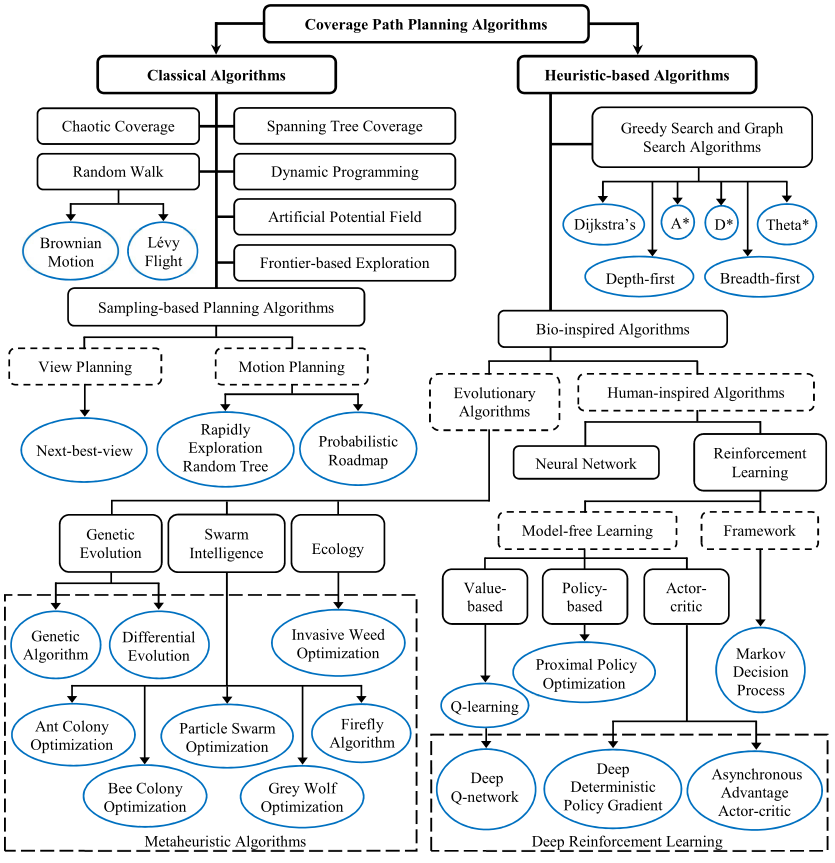
\includegraphics[height=22cm, width=\textwidth]{Images/general/general_classification.png}
    \caption{The classification of coverage path planning (CPP) algorithms.}
    \label{fig:classifications_of_CPP}
\end{figure}

\vspace{3mm}

Several algorithms relevant to coverage path planning for points or regions, which adhere to non-holonomic constraints with the objective of minimizing total route length, computational time, and energy consumption, are discussed below.


\subsection{Dubin's Path}

In the realm of geometric analysis and constrained path planning, the pioneering work of L.E. Dubins stands as a cornerstone, providing profound insights into the properties and characteristics of paths subject to curvature constraints. Dubins' seminal exploration, outlined in the paper \hyperlink{cite.dubins}{[1]}, lays a robust foundation for understanding the fundamental principles governing constrained path planning and provides critical insights into the properties of paths constrained by curvature.

\vspace{3mm}

At the core of Dubins' research lies the concept of R-geodesics, representing paths of minimal length under specified curvature constraints. This notion encapsulates the geometric essence of constrained paths, defining them as combinations of straight lines and circular arcs with a minimum radius of curvature, denoted as R. Dubins' theorem regarding the structure of R-geodesics in two dimensions provides a clear geometric understanding, asserting that such paths consist of no more than three segments, each comprising either a straight line or an arc of a circle with radius R. This theorem delineates the structure of minimal paths and imposes precise constraints on their composition, revealing the inherent simplicity of paths subject to curvature constraints.

\vspace{3mm}

Dubins rigorously proved the existence of R-geodesics using mathematical tools like Ascoli's theorem and concepts from E. Schmidt's proof of A. Schur's Lemma. These proofs confirm the theoretical existence of such paths and illuminate their analytical and geometric properties.

\vspace{3mm}

Dubins' work represents a significant milestone in the study of geometric analysis and constrained path planning, providing not only a solution to a specific geometric problem but also a methodological framework applicable to a broader class of problems in path planning and optimization. Therefore, many extensions of Dubins have been studied since then, integrating with other approaches to solve complex path planning problems. Due to its effectiveness towards curvature constraints and path length minimization, the Dubins path serves as a potential technique to inspire and inform further research into path planning algorithms for agricultural robots.


\subsection{Reeds-Shepp Paths}

Reeds-Shepp paths, introduced by J.A. Reeds and L.A. Shepp in the paper \hyperlink{cite.reeds}{[3]}, offers a flexible solution to optimal path planning for vehicles capable of moving forwards and backwards. Unlike Dubins paths, which only accommodate forward movement, Reeds-Shepp paths enhance maneuverability by incorporating reverse movements, doubling the range of possible maneuvers. This flexibility enables efficient navigation in complex environments, making them ideal for applications like robotics and autonomous vehicle navigation.

\vspace{3mm}

In agricultural robotics, Reeds-Shepp paths are particularly beneficial for tasks like weed removal, where precise navigation is essential. Their flexibility allows for efficient navigation through narrow spaces and around obstacles, reducing time and energy consumption. Reeds and Shepp's comprehensive analysis of Reeds-Shepp paths laid the foundation for subsequent research in optimal control and path planning, emphasizing the importance of considering a vehicle's full range of capabilities.





\subsection{Travelling Salesman Problem (TSP) with Neighborhoods} 

The Traveling Salesman Problem (TSP) represents a classic conundrum in optimization, challenging researchers to find the most efficient route for a salesman to visit a set of locations and return to the starting point while minimizing the total distance traveled. Renowned for its computational complexity and practical applications in logistics and route planning, the TSP has spurred numerous investigations into variants that more accurately reflect real-world scenarios.

\vspace{3mm}

One such variant, explored in the paper \hyperlink{cite.TSPN}{[4]}, introduces the concept of TSP with neighborhoods (TSPN). In this formulation, destinations are not singular points but rather areas or neighborhoods, complicating the problem by requiring the salesman to visit each neighborhood at least once without specifying exact points for each visit. TSPN is particularly relevant as it mirrors the challenge of navigating through regions (fields with weeds) rather than fixed points.

\vspace{3mm}

To address the challenges posed by TSPN, the paper introduces innovative approximation algorithms tailored to different types of neighborhoods, such as line segments or complex shapes described as "fat" regions. A notable contribution is the development of a constant factor approximation algorithm for neighborhoods represented as line segments, signifying a significant advancement in the field of geometric optimization.

\vspace{3mm}

A significant contribution of the paper is the m-guillotine method, which recursively subdivides the plane to approach a near-optimal solution. This method, along with key theoretical insights, underpins the algorithms' effectiveness in solving TSPN. However, it is essential to note that the TSPN problem is NP-hard, and the proposed algorithms provide only approximation solutions. While TSPN works with regions instead of points and strives to find the optimal solution, it does not explicitly consider the curvature constraints inherent in robotic path planning scenarios.











\subsection{Traveling Salesperson Problems for Dubins’ vehicle.}



After TSPN evolved from TSP, the challenges associated with optimal path planning for Dubins' vehicles, constrained by their minimum turning radius, have garnered significant attention. The paper \hyperlink{cite.TSP_with_dubins}{[5]} offers a thorough examination of these challenges and introduces innovative methodologies to overcome them.

\vspace{3mm}


At the core of this paper are two fundamental problems: the point-to-point shortest path problem (PTP) and the traveling salesperson problem (TSP) tailored for Dubins’ vehicles. These problems are crucial for developing algorithms capable of computing optimal or near-optimal paths for vehicles subject to nonholonomic constraints. the paper tackles the traveling salesperson problem (TSP) for Dubins’ vehicles, wherein the vehicle must visit a predefined set of locations in the most efficient route without revisiting any point. Acknowledging the computational complexity of exact solutions for larger point sets, the authors explore heuristic and approximation algorithms to efficiently approximate solutions.

\vspace{3mm}

The methodology outlined in the paper integrates rigorous mathematical frameworks and computational geometry to address the complexities of path planning for Dubins’ vehicles. By synthesizing Dubins constraints with the Traveling Salesperson Problem (TSP), the study offers a cohesive approach that bridges theoretical insights with practical solutions. this paper constitutes a significant contribution to the literature on path planning for nonholonomically constrained vehicles, paving the way for further advancements in navigating Dubins’ vehicles efficiently and effectively.











\subsection{Dubins Traveling Salesman Problem with Neighborhoods}

To address the challenges posed by regions in the Dubins Traveling Salesman Problem (DTSP), the paper \hyperlink{cite.DTSPN}{[6]} introduces a tailored formulation termed the Dubins Touring Regions Problem (DTRP). This novel approach aims to determine an optimal sequence of configurations for entering and exiting regions, all while minimizing the total path length. Unlike the conventional Traveling Salesman Problem (TSP), which focuses on finding the shortest route visiting a set of points, the DTSPN involves regions or neighborhoods, necessitating the vehicle to access each region at least once. This problem holds significant relevance in various applications, including autonomous drone surveillance, delivery systems, and robotic exploration, where vehicles must efficiently traverse specified areas while adhering to nonholonomic constraints.

\vspace{3mm}

The proposed algorithm for solving the DTRP leverages local iterative optimization techniques, taking into account the unique dynamics of Dubins vehicles. It begins with an initial sequence of region visits derived from solving an Euclidean TSP (ETSP), which serves as a proxy for the region centers. The algorithm then iteratively refines the entry and exit configurations to minimize the total tour length.

\vspace{3mm}

A key aspect of the solution method is its decoupled approach, optimizing the heading and position of each entry point independently. This simplification, facilitated by mathematical techniques that project the problem into a more manageable form, allows for efficient local optimization. The algorithm iterates until no further improvements can be made or a termination criterion is met, incorporating strategies to escape local minima by adjusting vehicle headings and repositioning at region boundaries.

\vspace{3mm}

Empirical validation of the algorithm demonstrates its effectiveness and efficiency across various scenarios, including different region shapes and configurations, particularly in dense environments where regions are close together. Comparative analysis against existing evolutionary algorithms showcases the proposed method's ability to produce high-quality solutions with significantly reduced computational time, making it suitable for real-time applications on modest hardware, such as onboard computers in UAVs.

\vspace{3mm}

Despite its capability to generate near-optimal paths while adhering to the non-holonomic constraints, the algorithm exhibits notable drawbacks in terms of computational efficiency. For instance, computing a near-optimal path for 30 regions may require over a minute, and the algorithm's performance further deteriorates with an increasing number of points, especially when they are closely positioned. Moreover, the algorithm's limitation in considering the overlap of regions represents a critical drawback, as it fails to account for this aspect in real-world scenarios, thereby impacting the path planning accuracy and efficiency.




\subsection{DTSPN with Overlappped Regions}



The paper \hyperlink{cite.overlap}{[7]} introduces the Intersecting Regions Algorithm (IRA) to address the challenges posed by intersecting regions in DTSPN. By explicitly considering the overlap among regions, IRA offers a more comprehensive solution compared to traditional methods. It leverages sampling within intersecting regions to construct feasible tours for autonomous vehicles, resulting in optimized route selection and more efficient path planning.

\vspace{3mm}

Furthermore, IRA reduces the computational complexity associated with path planning by adopting a polynomially scalable algorithmic structure. This scalability ensures IRA's viability even in scenarios with numerous regions of interest, where computational resources are limited. Monte Carlo simulations validate IRA's practical utility, showcasing significant performance enhancements, particularly in scenarios with high degrees of region overlap. However, despite its advancements, IRA still encounters challenges when dealing with a large number of points and close proximity points. These limitations highlight avenues for further research and development to enhance the algorithm's robustness and efficiency in addressing complex DTSPN scenarios.








\subsection{Path planning in confined spaces}


Navigating narrow and complex environments presents challenges for non-holonomic vehicles. In the paper \hyperlink{cite.mapping}{[8]}, the authors propose a path planning method tailored to address these challenges, focusing on generating paths with continuous curvature to ensure smooth operation in confined spaces.

\vspace{3mm}

The proposed method adopts a two-phase planning approach combining global and local strategies for efficient navigation. In the first phase, the authors employ the RTR (Rotate-Translate-Rotate) planner, a variation of the Rapidly Exploring Random Tree (RRT) method. This planner generates paths consisting of straight movements and in-place turning, simplifying complex maneuvering for navigating constrained spaces.

\vspace{3mm}

In the second phase, the global path is refined using the TTS local planning procedure. This planner approximates the initial path with a sequence of paths adhering to the vehicle's curvature constraints, ensuring smooth and feasible trajectories. The TTS planner can generate paths with continuous curvature turns (CC-turns) and straight segments, offering flexibility adaptable to various environmental constraints.

\vspace{3mm}

The paper also emphasizes maintaining similarity between global and local trajectories to avoid sudden changes in the path and ensure smooth passage through narrow regions. Ultimately, the objective is to enhance the capabilities of autonomous vehicles to operate safely and efficiently in diverse scenarios, thereby improving their practicality for everyday use.


\newpage

\section{Problem Statement}

We consider a robotic scenario wherein a four-wheel robot equipped with a mechanical CNC-inspired system for extraction operates within a defined area. The robot, characterized as non-holonomic, integrates the mechanical system beneath it, enabling movement along the x and y directions by approximately 60 cm, and vertically until ground contact. Due to its non-holonomic nature, the robot imposes kinematic constraints on turning, enforcing a minimum turning radius of 2 meters.

\vspace*{6mm} 


The operational environment comprises grass fields assumed to be uniform without any slopes (z=0), covering a real area of 120x90 square meters. Weed distribution within this area is heterogeneous, with approximately 60 percent of points clustered following a Gaussian distribution with varying variances. Weed positions are obtained via drone-based data collection, utilizing a deep learning model to identify weed locations. This dataset serves as the basis for complete coverage path planning.

\vspace*{6mm} 


Given the robot's mechanical implementation width of 60 cm, the operational region is discretized into points with each point representing an area of 30 cm, facilitating path planning optimization. The robot's velocity is constrained to 0.8 m/s on straight paths and 0.4 m/s on curved paths.

\vspace*{6mm} 


The primary objective of this research is to develop a path planning algorithm capable of covering all weed points within the designated area while adhering to the robot's non-holonomic constraints. Additionally, the algorithm aims to generate paths that approximate straight lines where feasible, ensuring comprehensive coverage of all points.

\vspace*{6mm} 

The objectives of the proposed algorithm include:

\begin{itemize}
    \item \textbf{Realistic Path Generation:} Develop paths that mimic natural movement patterns, enhancing operational realism.
    \item  \textbf{Computational Efficiency:} Minimize processing time and resources required for path planning.
    \item  \textbf{Energy Conservation:} Optimize energy consumption during path execution, enhancing overall operational efficiency.
    \item  \textbf{Field Operation Efficiency:} Facilitate efficient field operations, reducing time spent on weed detection and removal processes.
\end{itemize}

The algorithm should prioritize finding the shortest path distance to cover all weed points effectively while meeting the aforementioned objectives. The algorithm's performance will be evaluated based on the time taken to generate paths, the distance covered, and the energy consumed during path execution.

\vspace*{6mm} 


\newpage


\section{Experimental Setup}

\subsection{Environment}
The environment for our coverage motion planning algorithm is situated in a grass field characterized by small grass uniformly distributed across the area. The grass field is representative of typical agricultural settings, where weed management is essential for maintaining crop quality and productivity. As the grass matures, it is common for various unwanted plants, particularly weeds, to grow sporadically throughout the field. Our primary focus in this study is on the removal of Rumex (commonly known as dock weeds), which pose a significant challenge to farmers. However, the algorithm can be adapted to target other types of weeds based on specific requirements, the only that change would be the detection system to identify the target weed.

\subsection{Importance of Weed Removal}
Importance of Weed Removal
We are concentrating on Rumex plants due to their detrimental impact on agricultural productivity and livestock health. Although Rumex plants are not inherently toxic, their presence in cattle feed can adversely affect the quality of milk production. Ensuring the purity of grass fed to cattle is crucial for producing high-quality, bio milk, which is not only more beneficial for human consumption but also promotes better health and well-being of the cattle. Pure grass feed leads to higher nutritional value in milk, contributing to improved dairy products. Therefore, effective weed management, particularly the removal of Rumex plants, is essential for maintaining the quality and productivity of grass fields.


\vspace*{6mm} 


Traditionally, farmers have resorted to manually removing these weeds, a labor-intensive and time-consuming process. Manual removal becomes particularly arduous in large fields, imposing significant physical strain on farmers and limiting the efficiency of weed management. Automating this process with robotic systems offers a promising solution to enhance agricultural practices and improve farmers' quality of life.

\vspace*{6mm}

\subsection{The Robot}

\subsubsection{Overview}

To efficiently remove weeds from the grass field, we employ a robust, four-wheeled robot specifically designed for this task. This section provides an in-depth look at the robot's external and internal features, highlighting the components that enable it to navigate the field and execute precise weed extraction.

\subsubsection{External Features}

The robot features a four-wheeled design, ensuring stability and effective maneuverability across uneven terrain. The choice of a four-wheeled configuration is crucial as it supports the internal weed extraction system, which occupies most of the internal space. The wheels are equipped with treads suitable for grass fields, providing the necessary traction and mobility.

\vspace*{6mm}

\textbf{Localization and Orientation:} For accurate positioning and orientation in the open field, the robot is equipped with two Real-Time Kinematic (RTK) GPS systems. RTK GPS technology is ideal for this environment, offering centimeter-level accuracy in localization, which is essential for precise navigation and weed targeting.

\vspace*{6mm}


\textbf{Vision System:} The robot incorporates two strategically placed cameras. The front-facing camera is oriented towards the ground, scanning for weeds ahead of the robot. This early detection allows the local planner to adjust the robot's path accordingly, ensuring efficient navigation and weed targeting. The second camera is mounted at the bottom center of the robot, directly above the extraction mechanism. This camera provides an accurate view of the weed's position beneath the robot, facilitating precise extraction.


\subsubsection{Internal Features}

The internal mechanism of the robot is crucial for the precise and efficient removal of weeds. It comprises several key components: a processing unit, a battery system, and the main weed extraction system.


\vspace*{6mm}


\textbf{Processing Unit: } The processing unit serves as the brain of the robot, orchestrating the various functions and ensuring smooth operation. It processes data from the cameras and GPS systems, making real-time decisions to control the navigation and extraction processes. The unit is equipped with advanced algorithms for path planning, weed detection, and tool control, enabling the robot to perform its tasks autonomously and efficiently.


\vspace*{6mm}

\textbf{Battery System: }
The robot is powered by a robust battery system designed to provide sufficient energy for extended field operations. The battery pack is engineered for easy replacement, ensuring minimal downtime and continuous operation. This power system supports all onboard electronics, including the processing unit, cameras, GPS, and the weed extraction mechanism.


\vspace*{6mm}


\textbf{Weed Extraction System: }
The heart of the weed removal process is the weed extraction system, inspired by CNC machine technology. This system features two moving rails that allow the internal extraction mechanism to move in both the x and y directions. Controlled by the processing unit, these rails provide precise positioning capabilities. The extraction mechanism can move approximately 60 cm in both the x and y directions, covering a significant area beneath the robot. Once a weed is detected, the system moves the tool directly above the weed. The mechanical tool is then lowered in the negative z direction to engage the weed.

\vspace*{6mm}

The extraction tool is designed with sharp implements and rotates at high speed to destroy the weed effectively. This rotation ensures that the weed is thoroughly eradicated and cannot regrow. After destroying the weed, the remnants are left on the field, eliminating the need to carry them, which would otherwise burden the robot. The robot’s internal system, with its 60 cm movement range in both directions, allows for efficient navigation. Each detected weed point can be associated with a circular region within which the robot can maneuver to remove the weed. This approach not only aids in accurate weed extraction but also facilitates efficient path planning. By considering these regions, the planning algorithm can optimize the robot's path to cover all weed points effectively.

\vspace*{6mm}

\textbf{Adaptive Regions and Uncertainty Management: }
The regions around each weed point also serve to manage uncertainty in weed detection. If the position of a weed is detected with less accuracy, the associated region can be adjusted accordingly. A larger uncertainty reduces the size of the region to ensure the robot remains closer to the center, enhancing the likelihood of successful extraction. This adaptive approach allows the robot to handle variations in detection accuracy, maintaining high efficiency and precision in weed removal. The robot's internal features are meticulously designed to support the complex task of weed removal. The combination of precise movement capabilities, robust processing power, and adaptive region management ensures that the robot can effectively and efficiently eradicate weeds from the grass field.

\subsection{Constraints}

With a comprehensive understanding of the robot's capabilities and features, it is essential to delve into the constraints that arise due to its mechanical system and the nature of the field in which it operates. These constraints significantly influence the development of an effective motion planning algorithm.

\vspace*{6mm}

\textbf{Non-Holonomic Nature:}
The robot is equipped with four regular wheels, limiting its movement capabilities. Unlike holonomic robots, which can move in any direction, our robot cannot move sideways. It is constrained to forward and backward movements and must make turns to change its direction. This non-holonomic nature adds a layer of complexity to the motion planning algorithm, as it must account for the robot's inability to change its heading instantaneously.

\vspace*{6mm}

\textbf{Turning Radius:} The robot has a minimum turning radius of 2 meters, meaning it cannot make sharp turns. This constraint necessitates careful planning to ensure the robot can navigate around obstacles and reach all designated weed points without making turns that exceed its turning capabilities.

\vspace*{6mm}

\textbf{Speed Variations:} The robot's speed must be carefully regulated to prevent damage to the grass and ensure precise weed removal. When moving in a straight path, the robot operates at a velocity of 0.8 m/s. However, when making a turn, the velocity is reduced to 0.4 m/s to maintain the 2-meter turning radius. This adjustment helps in maintaining stability and accuracy during turns, which is critical for avoiding collateral damage to the grass and ensuring efficient weed extraction.

\vspace*{6mm}

\textbf{Kinematic Constraints:} Given its non-holonomic nature and the minimum turning radius, the robot cannot change its heading angle at a specific position. Instead, it requires a certain amount of space to turn and align itself in the desired direction. These kinematic constraints must be factored into the motion planning algorithm to ensure smooth and feasible navigation across the field.

\vspace*{6mm}

\textbf{Field Constraints:} The field is covered with grass and scattered weeds, particularly the rumex plants. The random distribution of weeds means the robot must navigate the entire field efficiently to locate and remove all weeds. The algorithm must account for this scattered distribution and plan paths that ensure comprehensive coverage without unnecessary overlaps.


\vspace*{6mm}



With a clear understanding of the robot's constraints, we can now proceed to develop a motion planning algorithm that leverages these constraints to ensure comprehensive and efficient weed removal. By integrating considerations for non-holonomic movement, adaptive speed control, optimized coverage, obstacle avoidance, and environmental adaptability, the algorithm will facilitate the robot's autonomous operation, making the weed removal process more efficient and reducing the burden on farmers. This strategic approach not only enhances the robot's performance but also contributes to maintaining the health of the grass and improving the overall quality of the field.

























\subsection{Remnants}


Benefits of Robotic Weed Removal
Deploying robots for weed removal in grass fields presents several advantages:

Increased Efficiency: Robots can operate continuously and systematically cover large areas, ensuring thorough removal of unwanted plants without fatigue.
Labor Savings: Automating weed removal reduces the need for manual labor, freeing farmers to focus on other essential tasks and reducing physical strain.
Precision: Advanced sensors and algorithms enable robots to identify and target specific weeds, minimizing damage to the surrounding grass and ensuring effective weed management.
Health Benefits: By eliminating the need for manual weed removal, farmers can avoid the physical exertion and potential health risks associated with prolonged exposure to outdoor conditions and repetitive movements.
Enhanced Livestock Health: Ensuring the purity of grass feed leads to healthier cattle, which in turn produce higher-quality milk, enhancing overall dairy production.


Experimental Objective
The primary objective of our experimental setup is to develop and validate a coverage motion planning algorithm that enables robots to efficiently navigate and manage weed removal in grass fields. By leveraging advanced robotic technology, we aim to automate the process of identifying and removing Rumex plants, ultimately improving agricultural productivity and promoting sustainable farming practices.

Methodology
The experimental setup involves the following key steps:

Field Analysis: Detailed mapping of the grass field to identify the distribution of grass and Rumex plants.
Algorithm Development: Creating a coverage motion planning algorithm tailored to navigate the field and target Rumex plants for removal.
Robotic Implementation: Equipping robots with necessary sensors and tools to detect and remove weeds, followed by field testing to ensure operational efficiency.
Performance Evaluation: Assessing the effectiveness of the robotic system in terms of coverage, weed removal accuracy, and operational efficiency.
By addressing the challenges of weed management through robotic automation, we aim to revolutionize agricultural practices, making farming more sustainable, efficient, and farmer-friendly. This innovative approach not only enhances the productivity of grass fields but also contributes to the overall well-being of livestock and farmers alike.
















Integrating Constraints into Motion Planning
Understanding the mechanical and field constraints is crucial for developing an effective coverage motion planning algorithm. These constraints guide the design of the algorithm to ensure it is practical and feasible under real-world conditions.

Path Planning with Non-Holonomic Constraints: The algorithm must plan paths that respect the robot's non-holonomic nature. This involves generating smooth, continuous paths that the robot can follow without needing to make sharp turns. Techniques such as Dubins curves, which are designed for non-holonomic vehicles, can be employed to create feasible paths that the robot can navigate.

Adaptive Speed Control: Incorporating variable speed control into the algorithm allows for safe and efficient navigation. The robot should move faster in straight paths to cover more ground quickly and slow down during turns to maintain stability and precision. This adaptive speed control also helps in preventing damage to the grass, ensuring that the robot's operations are minimally invasive.

Coverage Optimization: The algorithm should optimize the coverage pattern to ensure that all weeds are detected and removed efficiently. By considering the robot's 60 cm movement range in both directions, the algorithm can plan paths that cover larger areas without unnecessary backtracking. This optimization reduces the total time and energy required for weed removal.

Obstacle Avoidance and Navigation: The algorithm must include robust obstacle avoidance capabilities to navigate around natural terrain features and any unforeseen obstacles. This ensures the robot can continue its operation smoothly without interruptions.

Handling Environmental Variability: To ensure reliable performance under varying environmental conditions, the algorithm can incorporate sensor feedback to adjust the robot's path and speed in real-time. This adaptability enhances the robot's resilience and operational efficiency.
\newpage

\chapter{Methodology}

The main algorithm is comprised of two primary steps: data preprocessing and the behavior algorithm. In the data preprocessing phase, regions are converted into points by computing the centroids of their overlaps. The behavior algorithm phase utilizes these computed points to generate the complete path.

\section{Data Preprocessing}


Data preprocessing is a pivotal step in the research methodology, especially in the context of coverage path planning for weed removal in agricultural fields. This section delineates the comprehensive preprocessing procedures employed to ensure the precision and efficacy of the data used in the subsequent analysis.

\vspace{3mm}  


\textbf{Data Acquisition: }
The initial phase of preprocessing involves the acquisition of data pertaining to the weed positions within the field. This data collection is facilitated through the use of a drone for pinpointing the locations of weeds. The drone performs a systematic survey of the field, capturing high-resolution images to detect weed positions. The resultant data is then utilized as input for the coverage path planning module. Due to the developmental status of the drone, the current implementation involves manual data acquisition using a real-time kinematic GPS (RTK) system. The RTK system offers centimeter-level accuracy in pinpointing weed locations, which, for the purpose of this research, is considered sufficiently precise. 

\vspace{3mm}  


\textbf{Handling Data Uncertainty: }
In a practical scenario, the drone's output would include positional data of weeds along with an associated uncertainty measure, reflecting the inherent imprecision of the system. However, given the reliance on RTK data for this research phase, we assume perfect positional accuracy. This uncertainty measure will be used to define the regions of influence for each weed, ensuring that the coverage path planning algorithm accounts for the imprecision in the data. 


\vspace{3mm}  


\textbf{Region Definition and Overlap Management: } When data points from the drone indicate weed positions, these points often come with overlapping regions due to the growth patterns of weeds like Rumex, which tend to cluster.

\vspace{3mm}  


Overlap Reduction: To address overlaps, the preprocessing algorithm calculates the centroids of overlapping regions. Points within overlapping regions are consolidated to avoid duplication, ensuring that each weed cluster is represented by a single centroid. This consolidation reduces redundancy and enhances the efficiency of the coverage path planning.

\vspace{3mm}  


Non-Overlapping Weeds: For weeds whose regions do not overlap with others, the center of each weed is directly considered as a centroid. This step ensures that isolated weeds are accurately accounted for in the data set. The centroids of both overlapping and non-overlapping regions can be visualized in the \autoref{fig:overlape}. The green points represent the weeds, green circles represent the region of the weeds, and the red points represent the centroids of the regions. 

% selected field region.
\begin{figure}
    \centering
    \begin{tabular}{cc} 
        \begin{subfigure}{0.5\textwidth}
            \centering
            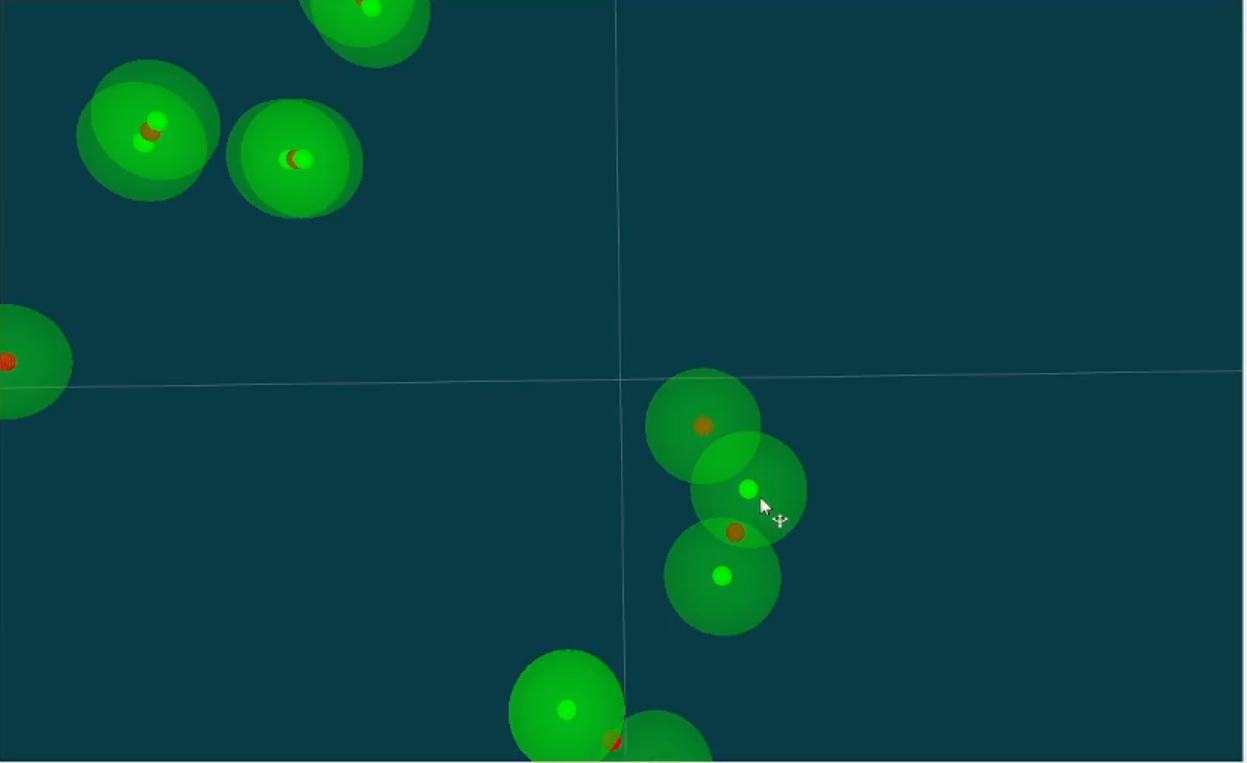
\includegraphics[width=\textwidth]{Images/Algorithm_no_obs/Centroid_1.png}
            % \caption{Selected Field Region}
        \end{subfigure} 
        &
        \begin{subfigure}{0.5\textwidth}
            \centering
            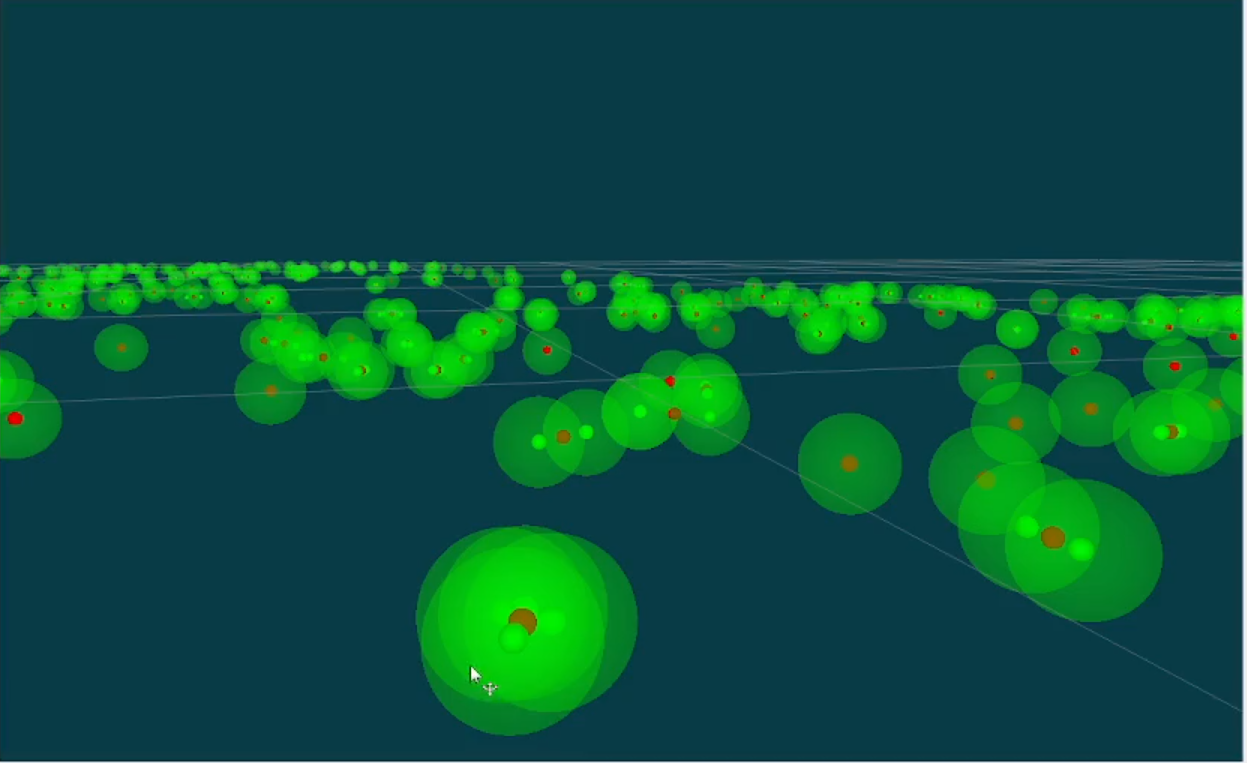
\includegraphics[width=\textwidth]{Images/Algorithm_no_obs/Centroid_2.png}
            % \caption{Points in the Region (Green)}
        \end{subfigure}
    \end{tabular}
    \caption{Centroids of overlapped regions.\label{fig:overlape}} 
\end{figure}

\vspace{3mm}  


\textbf{Data Integration and Optimization: }
By processing the data to identify centroids and manage overlaps, we achieve a significant reduction in the total number of points. Preliminary results indicate a reduction of at least 40\% in the number of data points, optimizing the dataset for coverage path planning. This reduction not only minimizes the total traversal length required for weed removal but also conserves energy and reduces redundant revisits.

\vspace{3mm}  


The processed data is then fed into the coverage path planning module, which utilizes the optimized set of points to devise an efficient path for weed removal, ensuring comprehensive coverage with minimal resource expenditure. The following figure illustrates the data preprocessing workflow, highlighting the steps taken to transform raw positional data into an optimized dataset ready for coverage path planning.

\vspace{3mm}  



This preprocessing approach ensures that the data fed into the coverage path planning algorithm is both accurate and efficient, laying a robust foundation for effective weed removal operations in agricultural fields.


\newpage



\subsection{Algorithm Description}

Behavioral Approach for Coverage Path Planning in Agricultural Fields

\vspace*{6mm}  

Following the preprocessing phase aimed at resolving the regions associated with designated points, the subsequent imperative lies in formulating an algorithm capable of comprehensively covering all identified points. With the completion of preprocessing, the focus narrows down to ensuring the precise coverage of all points to effectively identify and extract weed infestations. Although the agricultural robot in question operates under non-holonomic constraints, the overarching objective transcends mere efficiency and the identification of the shortest path. Instead, the primary emphasis lies in achieving exhaustive point coverage while strategically favoring approximately linear trajectories.

\vspace*{6mm}   

The rationale behind prioritizing linear trajectories over strictly adhering to non-holonomic paths is multifaceted. Firstly, the adoption of more curved paths significantly heightens the risk of grass damage, thereby undermining the fundamental objective of preserving grass quality. Given the paramount importance of maintaining optimal grass conditions within agricultural fields, any approach that compromises this aspect inherently fails to align with the core objectives. Secondly, the energy consumption associated with traversing curved paths is substantially higher compared to linear trajectories. For the specific agricultural robot under consideration, empirical estimates suggest that traversing an equivalent path length via curved trajectories incurs an energy expenditure four times greater than that of linear paths. Consequently, the central objective of the algorithm resides in identifying the shortest path capable of encompassing all designated points while mitigating curvature and prioritizing linear trajectories.

\vspace*{6mm}  

The development of this behavioral approach necessitates a nuanced understanding of agricultural terrain dynamics, robot kinematics, and energy efficiency considerations. By integrating these facets into the algorithmic design process, the resultant solution seeks to strike a delicate balance between point coverage efficacy, grass preservation, and energy optimization.

\vspace*{6mm}  


\textbf{Vision Cone Strategy: }

\vspace*{6mm}  


At this stage, having acquired comprehensive global information about the points in the field, the next step involves prioritizing straight paths while minimizing computational complexity and time. An innovative approach is employed wherein the robot is equipped with a vision cone mechanism. This vision cone is defined by two lines extending from the robot at a fixed angle and distance. The angle of these lines is determined based on the robot's minimum turning radius. For instance, for a robot with a minimum turning radius of 2 meters, the angle of the cone on either side is set at 11 degrees. The distance to the end of the cone depends on the operational area of the robot but is set to a fixed distance of 100 meters for this scenario.

\vspace*{6mm}  


The vision cone allows the robot to consider only those points within this cone from its current position as potential next travel points. This selective consideration significantly reduces the computational effort required to determine the path, as it disregards points outside the cone. By narrowing the focus to relevant points within the vision cone, computational efficiency is enhanced, thus making the vision cone an intelligent and effective strategy.

\vspace*{6mm}  


\textbf{Algorithmic Framework: }


\vspace*{6mm}  

The algorithmic framework is designed to facilitate comprehensive point coverage while minimizing curvature and prioritizing linear trajectories. The behavioral approach adopted for the algorithm is hierarchical, comprising three distinct behaviors that are sequentially activated. The transition from one behavior to the next is contingent upon the degree of point coverage achieved.

\begin{enumerate}
    \item \textbf{Initial Behavior: }The algorithm commences with the first behavior, designed to initiate coverage from the starting point. This stage focuses on covering a substantial portion of the field, leveraging the vision cone to select the next travel points and maintaining the priority on straight paths.
    
    \item \textbf{Intermediate Behavior:} Upon achieving a certain threshold of point coverage, the algorithm transitions to the second behavior. This intermediate stage aims to further optimize coverage by adjusting the strategy based on the points that remain. The robot continues to utilize the vision cone but adopt a slightly more flexible criteria for point selection to ensure efficient coverage progression.
    
    \item \textbf{Final Behavior:} Once the intermediate behavior reaches its saturation point—where additional coverage gains diminish—the algorithm shifts to the final behavior. This stage is designed to ensure complete, 100\% coverage of all remaining points. The final behavior will incorporate more refined strategies to target any residual areas, ensuring no point is left uncovered.
\end{enumerate}

\vspace*{6mm}   


This hierarchical behavioral algorithm ensures a methodical and efficient approach to coverage path planning. By starting with broad coverage strategies and progressively refining the approach, the algorithm effectively balances the need for comprehensive point coverage with the constraints of the robot's kinematic capabilities and the operational goal of preserving grass quality. The vision cone mechanism plays a pivotal role in this process, enhancing computational efficiency and enabling intelligent path selection. 

\vspace*{6mm}   


\textbf{Rationale for Hierarchical Approach: } 

\vspace*{6mm}   


The hierarchical approach is adopted to improve convergence rate and coverage efficiency. If a single algorithm or behavior were followed throughout, the robot would cover many points initially but gradually cover fewer points over time, reducing the algorithm's accuracy and increasing the overall path length and operational time. By transitioning between different behaviors, the algorithm can adapt to the changing density and distribution of points, maintaining high efficiency throughout the coverage process.

\vspace*{6mm}   


This hierarchical strategy ensures that the algorithm remains effective even as the number of uncovered points decreases. By tailoring the approach to the specific conditions encountered at each stage, the robot can optimize its path, reduce unnecessary movements, and maintain high precision in point coverage. This not only conserves energy but also preserves the quality of the grass by minimizing excessive traversal. The adaptive nature of the hierarchical approach thus represents a robust and efficient solution for coverage path planning in agricultural fields.

\vspace*{6mm}  

\subsubsection{First Behavior: Initial Coverage (change its name)}






\begin{algorithm}[H]
    \caption{CompleteBehavioralAlgorithm}
    \begin{algorithmic}[1]
        \Statex \textbf{Input:} 2D points, initial robot pose, turning radius
        \Statex \textbf{Output:} Dubins path
        \newline
        \State $clustered\_points, behavior\_change\_perc \gets CentroidsAndAutoBehaviorShift(2D points)$
        \State $remaining\_points \gets clustered\_points$ 
        \State $covered\_perc \gets 0$
        \State $completed\_path \gets []$
        \While{True}
            \If{$covered\_perc < behavior\_change\_perc$}
                \State $straight\_path, remaining\_points \gets Behavior\_1(remaining\_points, number\_of\_sample- $ \par
                \hspace{\algorithmicindent} $ -orientations (Ns), robot\_pose, vision\_cone, centroid,concurrent\_region\_radii, step) $ \par

                \State $completed\_path \mathrel{+}= straight\_path$
                \State $robot\_pose \gets completed\_path[-1]$
                \State $covered\_perc \gets UpdateCoveragePerc(clustered\_points, remaining\_points)$
            \Else
                \State $straight\_path, remaining\_points \gets Behavior\_2(remaining\_points, number\_of\_sample- $ \par
                \hspace{\algorithmicindent} $ -orientations (Ns), robot\_pose, vision\_cone, centroid,concurrent\_region\_radii, step) $ \par
                \State $completed\_path \mathrel{+}= straight\_path$
                \State $robot\_pose \gets completed\_path[-1]$
                \State $covered\_perc \gets UpdateCoveragePerc(completed\_path, remaining\_points)$
            \EndIf
            \If{$len(straight\_path) == 0$}
                \State \textbf{break}
            \EndIf
        \EndWhile
        \State $dubins\_path \gets DubinsPath(completed\_path, turning\_radius)$
        \State $dotsp\_path \gets DOTSPPath(remaining\_points, turning\_radius)$
        \State $complete\_dubins\_path \gets dubins\_path + dotsp\_path$
        \State \Return $complete\_dubins\_path$
    \end{algorithmic}
\end{algorithm}

Convention to be followed for the algorithms:
\begin{multicols}{2}
\begin{itemize}[noitemsep,topsep=0pt]
    \item $P$: path.
    \item $p$: points.
    \item $r$: robot.
    \item $R$: Radius.
    \item $VC$: Vision cone.
    \item $C$: Centroid.
    \item $N_s$: Number of sample orientations.
    \item $ \delta$: Percentage.
    \item $step$: Step size.
    \item $O$: Orientation.
\end{itemize}
\end{multicols}

\vspace*{6mm}  

Description of the notations:

\begin{multicols}{2}
\begin{itemize}[noitemsep,topsep=0pt]
    \item $p_{cl}$: clustered points.
    \item $p_r$: remaining points.
    \item $\delta_{\text{bc}}$: behavior change percentage.
    \item $\delta_c$: coverage percentage.
    \item $P_c$: completed path.
    \item $P_s$: straight path.
    \item $R_{\text{conc}}$: concurrent region radii.
    \item $P_d$: Dubins path.
    \item $P_{dotsp}$: DOTSP path.
    \item $P_cd$: Complete Dubins path.
\end{itemize}
\end{multicols}

\begin{algorithm}[H]
    \caption{CompleteBehavioralAlgorithm}
    \label{alg:completebehavioralalgorithm}
    \begin{algorithmic}[1]
    \Require 2D points ($p_{2d}$), initial robot pose ($r_{\text{pos}}$), turning radius ($R_{\text{tu}}$) 
    \Ensure Dubins path $P_{cd}$
    \State $p_{cl}, \delta_{\text{bc}} \leftarrow$ CentroidsAndAutoBehaviorShift($p_{2d}$)
    \State $p_r \leftarrow p_{cl}$
    \State $\delta_c \leftarrow 0$
    \State $P_c \leftarrow []$
    
    \While{True}
        \If{$\delta_c <  \delta_{\text{bc}}$}
            \State $P_s, p_r \leftarrow$ Behavior\_1($p_r$, $N_s$, $r_{\text{pos}}$, $VC$, $C$, $R_{\text{conc}}$, $step$)
        \Else
            \State $P_s, p_r \leftarrow$ Behavior\_2($p_r$, $N_s$, $r_{\text{pos}}$, $VC$, $C$, $R_{\text{conc}}$, $step$)
        \EndIf
        
        \State $P_c \mathrel{+}= P_s$
        \State $r_{\text{pos}} \leftarrow P_c[-1]$
        \State $\delta_c \leftarrow$ UpdateCoveragePerc($P_c$, $p_r$)
        
        \If{$\text{len}(P_s) == 0$}
            \State \textbf{break}
        \EndIf
    \EndWhile
    
    \State $P_d \leftarrow$ DubinsPath($P_c$, $R_{\text{tu}}$)
    \State $P_{dotsp} \leftarrow$ DOTSPPath($p_r$, $R_{\text{tu}}$)
    \State $P_{cd} \leftarrow P_d + P_{dotsp}$

    \State \Return $P_{cd}$
    \end{algorithmic}
\end{algorithm}
    

    

\begin{algorithm}[H]
    \caption{AutoBehaviorShift}
    \begin{algorithmic}[1]
    \Statex \textbf{Input: } \textit{2D points}, \textit{centroid}, \textit{min\_radius}, \textit{max\_radius}, number of concurrent circles (\textit{N}).
    \Statex \textbf{Output: }\textit{behavior\_change\_percent}
    \newline
    \State $total\_perc \gets 0$
    \State $threshold\_perc \gets 50$
    \State $percent\_list \gets \text{GeneratePercentageList}(30, 80, N)$ \Comment{List from 30 to 80\% with N steps.}
    \State $concentric\_circles \gets \text{ConcentricCircles}(points, min\_radius, max\_radius, N)$
    \For{$i, curr\_radius \in concentric\_circles$}
        \State $curr\_perc\_points \gets \text{PointsPercentageInSubregion}(curr\_radius)$
        \State $total\_perc \gets total\_perc + curr\_perc\_points$
        \If{$total\_perc > threshold\_perc$}
            \State $behavior\_change\_percent \gets percent\_list[i]$
            \State \textbf{break}
        \EndIf
    \EndFor
    \State \Return $behavior\_change\_percent$
    \end{algorithmic}
\end{algorithm}


Description of the notations:
\begin{multicols}{2}
    \begin{itemize}[noitemsep,topsep=0pt]
        \item $\delta_to$: Total percentage
        \item $\delta_{thp}$: Threshold percentage
        \item $\delta_{list}$: List of percentages
        \item $cc$: Concentric circles
        \item $R_{cu}$: Current radius
        \item $p_{cu_\delta}$: Percentage of points in subregion
    \end{itemize}
\end{multicols}

\begin{algorithm}[H]
    \caption{AutoBehaviorShift}
    \label{alg:autobehaviorshift}
    \begin{algorithmic}[1]
    \Statex \textbf{Input: }  $P_{2d}$, $R_{\text{min}}$, $R_{\text{max}}$, $N$ 
    \Statex \textbf{Output: } $\delta_{\text{bc}}$ 
    \newline
    \State $\delta_{to} \leftarrow 0$ 
    \State $\delta_{thp} \leftarrow 50$ 
    \State $\delta_{list} \leftarrow \text{GeneratePercentageList}(30, 80, N)$ \Comment{List from 30 to 80\% with N steps.}
    \State $cc \leftarrow \text{ConcentricCircles}(P_{2d}$, $R_{\text{min}}$, $R_{\text{max}}$, $N$)
    \For{$i, R_{cu}$ \textbf{in} $cc$}
        \State $p_{cu_\delta} \leftarrow \text{PointsPercentageInSubregion}(R_{cu})$
        \State $\delta_{to} \leftarrow \delta_{to} + p_{cu_\delta}$
        \If{$\delta_to > \delta_{thp}$}
            \State $\delta_{\text{bc}} \leftarrow \delta_{list}[i]$
            \State \textbf{break}
        \EndIf
    \EndFor
    \State \Return $\delta_{\text{bc}}$
    \end{algorithmic}
    \end{algorithm}
    

    
    
    
    



\begin{algorithm}[H]
    \caption{Behavioral1}
    \begin{algorithmic}[1]
        \Statex \textbf{Input:} 2D points, number of sample orientations $Ns$, robot pose, vision cone, centroid, concurrent region radii, step.
        \Statex \textbf{Output:} Complete path, remaining points.
        \newline
        \State $complete\_path \gets []$
        \State $temporary\_path \gets [[], [], [], ..., Ns]$
        \State $points\_covered \gets [[], [], [], ..., Ns]$
        \State $sample\_orientations \gets SampleTheOrientations(robot\_pose[2], Ns, step)$
        
        \For{$i, orientation$ in $sample\_orientations$}
            \State $robot\_pose[2] \gets orientation$
            \While{no point is visible}
                \State $visible\_points \gets ComputeVisionConePoints(robot\_pose, vision\_cone)$
                \State $potential\_point \gets FindPotentialPoint(robot\_pose, visible\_points)$
                \If{potential\_point is None}
                \State \textbf{break}
                \EndIf
                \State $new\_orientation \gets FromCurrentPoseToPotentialPoint(robot\_pose, potential\_point)$
                \State $temporary\_path[i].append([potential\_point, new\_orientation])$

                \State $Intermediate\_points \gets CheckIntermediatePoints()$
                \State $temporary\_path[i].append(Intermediate\_points)$
                \State $points\_covered[i].append(len(temporary\_path))$
                \State $remaining\_points \gets all\_points - temporary\_path$
                \State $robot\_pose \gets [potential\_point, new\_orientation]$
            \EndWhile
        \EndFor
        
        \State $best\_orientation\_index \gets \text{argmax}(points\_covered[:])$
        \State $complete\_path \gets temporary\_path[best\_orientation\_index]$
        
        \State $robot\_pose \gets complete\_path[-1]$
        \State $turn\_point \gets PotentialPointToTurn(remaining\_points, concurrent\_region\_radii, robot\_pose)$
        \State $best\_orientation \gets TowardsCentroid(turn\_point, centroid)$
        \State $complete\_path.append([turn\_point, best\_orientation])$
        \State $remaining\_points.remove([turn\_point])$

        \State \Return $complete\_path, remaining\_points$
    \end{algorithmic}
\end{algorithm}

Description of the notations:
\begin{multicols}{2}
    \begin{itemize}[noitemsep,topsep=0pt]
        \item $P_{cs}: Complete straight path$
        \item $P_{t}: Temporary path$
        \item $p_{co}: Points covered$
        \item $O_{sa}: Sampled orientations$
        \item $p_v: Visible points$
        \item $p_{po}: Potential point$
        \item $O_n: New orientation$
        \item $p_{int}: Intermediate points$
        \item $O_{bi}: Best orientation index$
        \item $P_{tu}: Turn point$
        \item $O_b: Best orientation$
    \end{itemize}
\end{multicols}

\begin{algorithm}[H]
    \caption{Behavioral1}
    \label{alg:behavioral1}
    \begin{algorithmic}[1]

    \Require Set of 2D points ($P_{2d}$), clustered points ($p_{cl}$), number of sample orientations ($N_s$), robot pose ($r_{pos}$), vision cone ($VC$), centroid ($C$), concurrent region radii ($R_{\text{conc}}$), step size ($S$)

    \Ensure Complete straight path $P_{cs}$, remaining points $p_r$
    \State $P_{cs} \leftarrow []$
    \State $P_t \leftarrow [[] \text{ for } \_ \text{ in range}(N_s)]$
    \State $p_{co} \leftarrow [[] \text{ for } \_ \text{ in range}(N_s)]$
    \State $O_{sa} \leftarrow$ SampleTheOrientations($R_{pos}[2]$, $N_s$, $S$)
    
    \For{$i, O$ \textbf{in} $O_{sa}$}
        \State $R_{pos}[2] \leftarrow O$
        \While{no point is visible}
            \State $p_v \leftarrow$ ComputeVisionConePoints($r_{pos}$, $VC$)
            \State $p_{po} \leftarrow$ FindPotentialPoint($r_{pos}$, $p_v$)
            \If{$p_{po}$ is None}
                \State \textbf{break}
            \EndIf
            \State $O_n \leftarrow$ FromCurrentPoseToPotentialPoint($r_{pos}$, $p_{po}$)
            \State $P_t[i].\text{append}([p_{po}, O_n])$
            
            \State $p_{int} \leftarrow$ CheckIntermediatePoints($p_r$)
            \State $P_t[i].\text{append}(p_{int})$
            \State $p_c[i].\text{append}(\text{len}(P_t))$
            \State $p_r \leftarrow p_{cl} - P_t$
            \State $r_{pos} \leftarrow [p_{po}, O_n]$
        \EndWhile
    \EndFor
    
    \State $O_{bi} \leftarrow \text{argmax}(p_c[:])$
    \State $P_{cs} \leftarrow P_t[O_{bi}]$
    
    \State $r_{pos} \leftarrow P_{cs}[-1]$
    \State $p_{tu} \leftarrow$ PotentialPointToTurn($p_r$, $R_{\text{conc}}$, $r_{pos}$)
    \State $O_b \leftarrow$ TowardsCentroid($p_{tu}$, $C$)
    \State $P_{cs}.\text{append}([p_{tu}, O_b])$
    \State $p_r.\text{remove}([p_{tu}])$
    
    \State \Return $P_{cs}$, $p_r$
    \end{algorithmic}
    \end{algorithm}
    

    


\begin{algorithm}[H]
    \caption{Behavioral2}
    \begin{algorithmic}[1]
        \Statex \textbf{Input:} Set of 2D points, number of sample orientations $Ns$, robot pose, vision cone, centroid, concurrent region radii, step
        \Statex \textbf{Output:} Complete path, remaining points
        \newline
        \State $complete\_path \gets []$
        \State $temporary\_path \gets [[], [], [], ..., Ns]$
        \State $points\_covered \gets [[], [], [], ..., Ns]$
        \State $sample\_orientations \gets SampleTheOrientations(robot\_pose[2], Ns, step)$
        
        \For{$i, orientation$ in $sample\_orientations$}
            \State $robot\_pose[2] \gets orientation$
            \While{no point is visible}
                \State $visible\_points \gets ComputeVisionConePoints(robot\_pose, vision\_cone)$
                \State $potential\_point \gets FindPotentialPoint(robot\_pose, visible\_points)$
                \If{potential\_point is None}
                    \State \textbf{break}
                \EndIf
                \State $new\_orientation \gets FromCurrentPoseToPotentialPoint(robot\_pose, potential\_point)$
                \State $temporary\_path[i].append([potential\_point, new\_orientation])$
                \State $Intermediate\_points \gets CheckIntermediatePoints()$
                \State $temporary\_path[i].append(Intermediate\_points)$
                \State $points\_covered[i].append(len(temporary\_path))$
                \State $remaining\_points \gets all\_points - temporary\_path$
                \State $robot\_pose \gets [potential\_point, new\_orientation]$
            \EndWhile
        \EndFor
        
        \State $best\_orientation\_index \gets \text{argmax}(points\_covered[:])$
        \State $complete\_path \gets temporary\_path[best\_orientation\_index]$
        
        \State $turn\_point \gets PotentialPointToTurnCCW(remaining\_points, concurrent\_region\_radii, robot\_pose)$
        \State $best\_orientation \gets VectorsTowardsNextCCWPoint(turn\_point, remaining\_points)$
        \State $complete\_path.append([turn\_point, best\_orientation])$
        
        \State \Return $complete\_path, remaining\_points$
    \end{algorithmic}
\end{algorithm}


\begin{algorithm}[H]
    \caption{Behavioral2}
    \label{alg:behavioral2}
    \begin{algorithmic}[1]

    \Require Set of 2D points ($P_{2d}$), clustered points ($p_{cl}$), number of sample orientations ($N_s$), robot pose ($r_{pos}$), vision cone ($VC$), centroid ($C$), concurrent region radii ($R_{\text{conc}}$), step size ($S$)

    \Ensure Complete straight path $P_{cs}$, remaining points $p_r$
    \State $P_{cs} \leftarrow []$
    \State $P_t \leftarrow [[] \text{ for } \_ \text{ in range}(N_s)]$
    \State $p_{co} \leftarrow [[] \text{ for } \_ \text{ in range}(N_s)]$
    \State $O_{sa} \leftarrow$ SampleTheOrientations($R_{pos}[2]$, $N_s$, $S$)
    
    \For{$i, O$ \textbf{in} $O_{sa}$}
        \State $R_{pos}[2] \leftarrow O$
        \While{no point is visible}
            \State $p_v \leftarrow$ ComputeVisionConePoints($r_{pos}$, $VC$)
            \State $p_{po} \leftarrow$ FindPotentialPoint($r_{pos}$, $p_v$)
            \If{$p_{po}$ is None}
                \State \textbf{break}
            \EndIf
            \State $O_n \leftarrow$ FromCurrentPoseToPotentialPoint($r_{pos}$, $p_{po}$)
            \State $P_t[i].\text{append}([p_{po}, O_n])$
            
            \State $p_{int} \leftarrow$ CheckIntermediatePoints($p_r$)
            \State $P_t[i].\text{append}(p_{int})$
            \State $p_c[i].\text{append}(\text{len}(P_t))$
            \State $p_r \leftarrow p_{cl} - P_t$
            \State $r_{pos} \leftarrow [p_{po}, O_n]$
        \EndWhile
    \EndFor
    
    \State $O_{bi} \leftarrow \text{argmax}(p_c[:])$
    \State $P_{cs} \leftarrow P_t[O_{bi}]$
    
    \State $r_{pos} \leftarrow P_{cs}[-1]$
    \State $p_{tu} \leftarrow$ PotentialPointToTurnCCW($p_r$, $R_{\text{conc}}$, $r_{pos}$)
    \State $O_b \leftarrow$ VectorsTowardsNextCCWPoint($p_{tu}$, $p_r$)
    \State $P_{cs}.\text{append}([p_{tu}, O_b])$
    \State $p_r.\text{remove}([p_{tu}])$

    \State \Return $P_{cs}$, $p_r$
    \end{algorithmic}
    \end{algorithm}
    

    



\begin{algorithm}[H]
    \caption{DOTSPPath}
    \begin{algorithmic}[1]
        \Statex \textbf{Input:} Set of 2D points, initial robot position, turning radius
        \Statex \textbf{Output:} Dubins path
        \newline
        \State $start\_node \gets initial\_robot\_position$
        \State $Graph \gets GenerateGraph(2D\_points)$
        \State $Closed\_path \gets SolveClosedTSP(Graph, start\_node)$
        \State $open\_path \gets RemoveEdgeWithMaxWeightFromStartNode(Graph, start\_node)$
        
        \State $dubins\_path \gets DubinsPath(open\_path, turning\_radius)$
        
        \State \Return $dubins\_path$
    \end{algorithmic}
\end{algorithm}

Description of the notations:
\begin{multicols}{2}
\begin{itemize}[noitemsep,topsep=0pt]
    \item $sn$: Start node
    \item $G$: Graph
    \item $P_{clo}$: Closed path
    \item $P_{op}$: Open path
    \item $P_d$: Dubins path
\end{itemize}
\end{multicols}

\begin{algorithm}[H]
    \caption{DOTSPPath}
    \label{alg:dotsp_path}
    \begin{algorithmic}[1]
    \Require Set of 2D points $P_{2d}$, initial robot position $r_{\text{pos}}$, turning radius $R_{\text{tu}}$
    \Ensure Dubins path $P_d$
    \State $sn \leftarrow r_{\text{pos}}$
    \State $G \leftarrow$ GenerateGraph($P_{2d}$)
    \State $P_{clo} \leftarrow$ SolveClosedTSP($G$, $sn$)
    \State $P_{op} \leftarrow$ RemoveEdgeWithMaxWeightFromStartNode($G$, $sn$)
    \State $P_d \leftarrow$ DubinsPath($P_{op}$, $R_{\text{tu}}$)
    \State \Return $P_d$
    \end{algorithmic}
    \end{algorithm}
    

    


































Convention to be followed for the algorithms:
\begin{multicols}{2}
\begin{itemize}[noitemsep,topsep=0pt]
    \item $OB$: Obstacle.
    \item $OB_p$: Polygonal obstacles.
    \item $OB_e$: Extended obstacles.
    \item $g$: grid.
    \item $g_s$: grids.
    \item $p_{bu}$: Buffer points.
    \item $G$: Graph.
    \item $S$: Step.
    \item $SP$: Salient Point.
    \item $P_{re}$: Remaining path.
\end{itemize}
\end{multicols}
    



\begin{algorithm}[H] 
    \caption{CompleteBehavioralObstacleAvoidance}
    \begin{algorithmic}[1]
        \Statex \textbf{Input:} 2D points, initial robot pose, turning radius, polygonal obstacles, grid diameter, vision cone
        \Statex \textbf{Output:} Dubins path
        \newline
        \State $extended\_obstacles, grids, buffer\_points \gets SetupObstacles(polygonal\_obstacles,$
        \Statex \hspace{9cm} $grid\_diameter, vision\_cone)$

        \State $extended\_obstacles, grids, buffer\_points \gets SetupObstacles(polygonal\_obstacles, $
        \Statex \hspace{9cm} $grid\_diameter, vision\_cone)$
        \State $clustered\_points, behavior\_change\_percentage \gets CentroidsAndAutoBehaviorShi f t(2Dpoints)$
        \State $remaining\_points \gets clustered\_points$
        \State $covered\_percentage \gets 0$
        \State $completed\_path \gets []$
        \While{True}
            \If{$covered\_percentage < behavior\_change\_percentage$}
                \State $straight\_path, remaining\_points \gets Behavioral1(extended\_obstacles, grids, buffer\_points,$
                \Statex \hspace{\algorithmicindent} $remaining\_points, Ns, robot\_pose, vision\_cone, centroid, concurrent\_region\_radii, step)$
                \State $completed\_path \mathrel{+}= straight\_path$
                \State $robot\_pose \gets completed\_path[-1]$
                \State $covered\_percentage \gets UpdateCoveragePercentage(clustered\_points, remaining\_points)$
            \Else
                \State $straight\_path, remaining\_points \gets Behavioral2(extended\_obstacles, grids, buffer\_points,$
                \Statex \hspace{\algorithmicindent} $remaining\_points, Ns, robot\_pose, vision\_cone, centroid, concurrent\_region\_radii, step)$
                \State $completed\_path \mathrel{+}= straight\_path$
                \State $robot\_pose \gets completed\_path[-1]$
                \State $covered\_percentage \gets UpdateCoveragePercentage(completed\_path, remaining\_points)$
            \EndIf
            \If{$\text{len}(straight\_path) == 0$}
                \State \textbf{break}
            \EndIf
        \EndWhile
        \State $dubins\_path \gets DubinsPath(completed\_path, turning\_radius)$
        \State $remaining\_path \gets PathAroundObstaclesAlgorithm(remaining\_points, turning\_radius)$
        \State $complete\_dubins\_path \gets dubins\_path + remaining\_path$
        \State \Return $complete\_dubins\_path$
    \end{algorithmic}
\end{algorithm}



\begin{algorithm}[H]
    \caption{CompleteBehavioralAlgorithm}
    \label{alg:complete_behavioral_obstacle_avoidance}
    \begin{algorithmic}[1]
    \Require 2D points ($p_{2d}$), initial robot pose ($r_{\text{pos}}$), turning radius ($R_{\text{tu}}$), polygonal obstacles ($OB_p$), grid diameter ($g_d$), vision cone ($VC$) 
    \Ensure Dubins path $P_{cd}$

    \State $OB_e, g_s, p_{bu} \leftarrow$ SetupObstacles($OB_p$, $g_d$, $VC$)
    \State $p_{cl}, \delta_{\text{bc}} \leftarrow$ CentroidsAndAutoBehaviorShift($p_{2d}$)
    \State $p_r \leftarrow p_{cl}$
    \State $\delta_c \leftarrow 0$
    \State $P_c \leftarrow []$
    
    \While{True}
        \If{$\delta_c <  \delta_{\text{bc}}$}
            \State $P_s, p_r \leftarrow$ Behavior\_1($OB_p$, $g_d$, $p_{bu}$, $p_r$, $N_s$, $r_{\text{pos}}$, $VC$, $C$, $R_{\text{conc}}$, $step$)
        \Else
            \State $P_s, p_r \leftarrow$ Behavior\_2($OB_p$, $g_d$, $p_{bu}$, $p_r$, $N_s$, $r_{\text{pos}}$, $VC$, $C$, $R_{\text{conc}}$, $step$)
        \EndIf
        
        \State $P_c \mathrel{+}= P_s$
        \State $r_{\text{pos}} \leftarrow P_c[-1]$
        \State $\delta_c \leftarrow$ UpdateCoveragePerc($P_c$, $p_r$)
        
        \If{$\text{len}(P_s) == 0$}
            \State \textbf{break}
        \EndIf
    \EndWhile
    
    \State $P_d \leftarrow$ DubinsPath($P_c$, $R_{\text{tu}}$)
    \State $P_{re} \leftarrow$ PathAroundObstaclesAlgorithm($p_r$, $R_{\text{tu}}$)
    \State $P_{cd} \leftarrow P_d + P_{re}$

    \State \Return $P_{cd}$
    \end{algorithmic}
\end{algorithm}


% \begin{algorithm}[H]
%     \caption{CompleteBehavioralObstacleAvoidance}
%     \label{alg:complete_behavioral_obstacle_avoidance}
%     \begin{algorithmic}[1]
%     \Require Set of 2D points $P$, initial robot pose $R_{\text{init}}$, turning radius $R_{\text{turn}}$, polygonal obstacles $O$, grid diameter $D_{\text{grid}}$, vision cone $VC$
%     \Ensure Dubins path $D$
%     \State $eo, g, bp \leftarrow$ SetupObstacles($O$, $D_{\text{grid}}$, $VC$)
%     \State $cp, bcp \leftarrow$ CentroidsAndAutoBehaviorShift($P$)
%     \State $rp \leftarrow cp$
%     \State $cp \leftarrow 0$
%     \State $cpd \leftarrow []$
    
%     \While{True}
%         \If{$cp < bcp$}
%             \State $sp, rp \leftarrow$ Behavioral1($eo$,$g$, $bp$, $rp$, $Ns$, $R_{\text{init}}$, $VC$, $centroid$, $concurrent\_region\_radii$, $step$)
%         \Else
%             \State $sp, rp \leftarrow$ Behavioral2($eo$,$g$, $bp$, $rp$, $Ns$, $R_{\text{init}}$, $VC$, $centroid$, $concurrent\_region\_radii$, $step$)
%         \EndIf
        
%         \State $cpd \mathrel{+}= sp$
%         \State $R_{\text{init}} \leftarrow cpd[-1]$
%         \State $cp \leftarrow$ UpdateCoveragePercentage($cp$, $rp$)
        
%         \If{$\text{len}(sp) == 0$}
%             \State \textbf{break}
%         \EndIf
%     \EndWhile
    
%     \State $dp \leftarrow$ DubinsPath($cpd$, $R_{\text{turn}}$)
%     \State $rp \leftarrow$ PathAroundObstaclesAlgorithm($rp$, $R_{\text{turn}}$)
%     \State $D \leftarrow dp + rp$
%     \State \Return $D$
%     \end{algorithmic}
%     \end{algorithm}
    


    






\begin{algorithm}[H]
    \caption{Behavioral1}
    \begin{algorithmic}[1]
        \Statex \textbf{Input:} Extended polygonal obstacles, grids, set of 2D points, number of sample orientations \textit{Ns}, robot pose, vision cone, centroid, concurrent region radii, step
        \Statex \textbf{Output:} Complete path, remaining points
        \newline
        \State $complete\_path \gets []$
        \State $temporary\_path \gets [[], [], [], \ldots, Ns]$
        \State $points\_covered \gets [[], [], [], \ldots, Ns]$
        \State $sample\_orientations \gets SampleTheOrientations(robot\_pose[2], Ns, step)$
        \For{$i, orientation \in sample\_orientations$}
            \State $robot\_pose[2] \gets orientation$
            \While{no point is visible}
                \State $visible\_points \gets ComputeVisionConePoints(robot\_pose, vision\_cone)$
                \State $potential\_point \gets FindPotentialPoint(robot\_pose, visible\_points)$
                \If{$potential\_point$ is None}
                    \State \textbf{break}
                \EndIf
                \State $new\_orientation \gets FromCurrentPoseToPotentialPoint(robot\_pose, potential\_point)$
                \State $curr\_path \gets [[robot\_pose, potential\_point]]$
                \State $obstacle\_free\_path \gets ComputeObstacleFreePath(curr\_path, new\_orientation)$
                \State $temporary\_path[i] \mathrel{+}= obstacle\_free\_path$
                \State $Intermediate\_points \gets CheckIntermediatePoints()$
                \State $temporary\_path[i].append(Intermediate\_points)$
                \State $points\_covered[i].append(len(temporary\_path))$
                \State $remaining\_points \gets all\_points - temporary\_path$
                \State $robot\_pose \gets obstacle\_free\_path[-1]$
            \EndWhile
        \EndFor
        \State $best\_orientation\_index \gets argmax(points\_covered[:])$
        \State $complete\_path \gets temporary\_path[best\_orientation\_index]$
        \State $robot\_pose \gets complete\_path[-1]$
        \State $turn\_point \gets PotentialPointToTurn(remaining\_points, concurrent\_region\_radii, robot\_pose)$
        \State $best\_orientation \gets TowardsCentroid(turn\_point, centroid)$
        \State $curr\_path \gets [[robot\_pose, turn\_point]]$
        \State $obstacle\_free\_path \gets ComputeObstacleFreePath(curr\_path, best\_orientation)$
        \State $complete\_path \mathrel{+}= obstacle\_free\_path$
        \State $remaining\_points.remove(obstacle\_free\_path)$
        \State \Return $complete\_path, remaining\_points$
    \end{algorithmic}
\end{algorithm}


Description of the notations:
\begin{itemize}[noitemsep,topsep=0pt]
    \item $P_{cu}$: Current path
    \item $P_{OB free}$: Obstacle free path
\end{itemize}

\begin{algorithm}[H]
    \caption{Behavioral1}
    \label{alg:behavioral1}
    \begin{algorithmic}[1]

    \Require Extended polygonal obstacles ($OB_p$), grids ($g_d$), buffer points ($p_{bu}$), Set of 2D points ($P_{2d}$), clustered points ($p_{cl}$), number of sample orientations ($N_s$), robot pose ($r_{pos}$), vision cone ($VC$), centroid ($C$), concurrent region radii ($R_{\text{conc}}$), step size ($S$)

    \Ensure Complete straight path $P_{cs}$, remaining points $p_r$
    \State $P_{cs} \leftarrow []$
    \State $P_t \leftarrow [[] \text{ for } \_ \text{ in range}(N_s)]$
    \State $p_{co} \leftarrow [[] \text{ for } \_ \text{ in range}(N_s)]$
    \State $O_{sa} \leftarrow$ SampleTheOrientations($R_{pos}[2]$, $N_s$, $S$)
    
    \For{$i, O$ \textbf{in} $O_{sa}$}
        \State $R_{pos}[2] \leftarrow O$
        \While{no point is visible}
            \State $p_v \leftarrow$ ComputeVisionConePoints($r_{pos}$, $VC$)
            \State $p_{po} \leftarrow$ FindPotentialPoint($r_{pos}$, $p_v$)
            \If{$p_{po}$ is None}
                \State \textbf{break}
            \EndIf
            \State $O_n \leftarrow$ FromCurrentPoseToPotentialPoint($r_{pos}$, $p_{po}$)
            \State $P_{cu} \leftarrow$ [[$r_{pos}$, $p_{po}$]]
            \State $P_{OB free} \leftarrow$ ComputeObstacleFreePath($P_{cu}$, $O_n$)


            \State $P_t[i] \mathrel{+}= P_{OB free}$
            
            \State $p_{int} \leftarrow$ CheckIntermediatePoints($p_r$)
            \State $P_t[i].\text{append}(p_{int})$
            \State $p_c[i].\text{append}(\text{len}(P_t))$
            \State $p_r \leftarrow p_{cl} - P_t$
            \State $r_{pos} \leftarrow P_{OB free}[-1]$
        \EndWhile
    \EndFor
    
    \State $O_{bi} \leftarrow \text{argmax}(p_c[:])$
    \State $P_{cs} \leftarrow P_t[O_{bi}]$
    
    \State $r_{pos} \leftarrow P_{cs}[-1]$
    \State $p_{tu} \leftarrow$ PotentialPointToTurn($p_r$, $R_{\text{conc}}$, $r_{pos}$)
    \State $O_b \leftarrow$ TowardsCentroid($p_{tu}$, $C$)

    \State $P_{cu} \leftarrow$ [[$r_{pos}$, $p_{tu}$]]
    \State $P_{OB free} \leftarrow$ ComputeObstacleFreePath($P_{cu}$, $O_b$)

    \State $P_{cs} \mathrel{+}= P_{OB free}$
    \State $p_r.\text{remove}([P_{OB free}])$ 
    
    \State \Return $P_{cs}$, $p_r$
    \end{algorithmic}
    \end{algorithm}




% \begin{algorithm}[H]
%     \caption{Behavioral1}
%     \label{alg:behavioral1}
%     \begin{algorithmic}[1]
%     \Require Extended polygonal obstacles $EO$, grids $G$, set of 2D points $P$, number of sample orientations $Ns$, robot pose $R$, vision cone $VC$, centroid $C$, concurrent region radii $R_{\text{conc}}$, step size $S$
%     \Ensure Complete path $CP$, remaining points $RP$
%     \State $cp \leftarrow []$
%     \State $tp \leftarrow [[] \text{ for } \_ \text{ in range}(Ns)]$
%     \State $pc \leftarrow [[] \text{ for } \_ \text{ in range}(Ns)]$
%     \State $so \leftarrow$ SampleTheOrientations($R[2]$, $Ns$, $S$)
    
%     \For{$i, o$ \textbf{in} $so$}
%         \State $R[2] \leftarrow o$
%         \While{no point is visible}
%             \State $vp \leftarrow$ ComputeVisionConePoints($R$, $VC$)
%             \State $pp \leftarrow$ FindPotentialPoint($R$, $vp$)
%             \If{$pp$ is None}
%                 \State \textbf{break}
%             \EndIf
%             \State $no \leftarrow$ FromCurrentPoseToPotentialPoint($R$, $pp$)
%             \State $cpn \leftarrow [[R, pp]]$
%             \State $ofp \leftarrow$ ComputeObstacleFreePath($cpn$, $no$)
%             \State $tp[i] \mathrel{+}= ofp$
%             \State $ip \leftarrow$ CheckIntermediatePoints()
%             \State $tp[i].\text{append}(ip)$
%             \State $pc[i].\text{append}(\text{len}(tp))$
%             \State $RP \leftarrow P - tp$
%             \State $R \leftarrow$ ofp[-1]
%         \EndWhile
%     \EndFor
    
%     \State $boi \leftarrow \text{argmax}(pc[:])$
%     \State $cp \leftarrow tp[boi]$
%     \State $R \leftarrow cp[-1]$
%     \State $tp \leftarrow$ PotentialPointToTurn($RP$, $R_{\text{conc}}$, $R$)
%     \State $bo \leftarrow$ TowardsCentroid($tp$, $C$)
%     \State $cpn \leftarrow [[R, tp]]$
%     \State $ofp \leftarrow$ ComputeObstacleFreePath($cpn$, $bo$)
%     \State $cp \mathrel{+}= ofp$
%     \State $RP.\text{remove}(ofp)$
%     \State \Return $cp$, $RP$
%     \end{algorithmic}
%     \end{algorithm}
    

    








\begin{algorithm}[H]
    \caption{BehavioralAlgorithm2}
    \begin{algorithmic}[1]
        \Statex \textbf{Input:} Extended polygonal obstacles, grids, set of 2D points, number of sample orientations \textit{Ns}, robot pose, vision cone, centroid, concurrent region radii, step
        \Statex \textbf{Output:} Complete path, remaining points
        \newline
        \State $complete\_path \gets []$
        \State $temporary\_path \gets [[], [], [], \ldots, Ns]$
        \State $points\_covered \gets [[], [], [], \ldots, Ns]$
        \State $sample\_orientations \gets SampleTheOrientations(robot\_pose[2], Ns, step)$
        \For{$i, orientation \in sample\_orientations$}
            \State $robot\_pose[2] \gets orientation$
            \While{no point is visible}
                \State $visible\_points \gets ComputeVisionConePoints(robot\_pose, vision\_cone)$
                \State $potential\_point \gets FindPotentialPoint(robot\_pose, visible\_points)$
                \If{$potential\_point$ is None}
                    \State \textbf{break}
                \EndIf
                \State $new\_orientation \gets FromCurrentPoseToPotentialPoint(robot\_pose, potential\_point)$
                \State $curr\_path \gets [[robot\_pose, potential\_point]]$
                \State $obstacle\_free\_path \gets ComputeObstacleFreePath(curr\_path, new\_orientation)$
                \State $temporary\_path[i] \mathrel{+}= obstacle\_free\_path$
                \State $Intermediate\_points \gets CheckIntermediatePoints()$
                \State $temporary\_path[i].append(Intermediate\_points)$
                \State $points\_covered[i].append(len(temporary\_path))$
                \State $remaining\_points \gets all\_points - temporary\_path$
                \State $robot\_pose \gets obstacle\_free\_path[-1]$
            \EndWhile
        \EndFor
        \State $best\_orientation\_index \gets argmax(points\_covered[:])$
        \State $complete\_path \gets temporary\_path[best\_orientation\_index]$
        \State $robot\_pose \gets complete\_path[-1]$
        \State $turn\_point \gets PotentialPointToTurnCCW(remaining\_points, concurrent\_region\_radii, robot\_pose)$
        \State $best\_orientation \gets VectorsTowardsNextCCWPoint(turn\_point, remaining\_points)$
        \State $curr\_path \gets [[robot\_pose, turn\_point]]$
        \State $obstacle\_free\_path \gets ComputeObstacleFreePath(curr\_path, best\_orientation)$
        \State $complete\_path \mathrel{+}= obstacle\_free\_path$
        \State $remaining\_points.remove(obstacle\_free\_path)$
        \State \Return $complete\_path, remaining\_points$
    \end{algorithmic}
\end{algorithm}


\begin{algorithm}[H]
    \caption{BehavioralAlgorithm2}
    \label{alg:behavioral_algorithm_2}
    \begin{algorithmic}[1]

    \Require Extended polygonal obstacles ($OB_e$), grids ($g_d$), buffer points ($p_{bu}$), Set of 2D points ($P_{2d}$), clustered points ($p_{cl}$), number of sample orientations ($N_s$), robot pose ($r_{pos}$), vision cone ($VC$), centroid ($C$), concurrent region radii ($R_{\text{conc}}$), step size ($S$)

    \Ensure Complete straight path $P_{cs}$, remaining points $p_r$
    \State $P_{cs} \leftarrow []$
    \State $P_t \leftarrow [[] \text{ for } \_ \text{ in range}(N_s)]$
    \State $p_{co} \leftarrow [[] \text{ for } \_ \text{ in range}(N_s)]$
    \State $O_{sa} \leftarrow$ SampleTheOrientations($R_{pos}[2]$, $N_s$, $S$)
    
    \For{$i, O$ \textbf{in} $O_{sa}$}
        \State $R_{pos}[2] \leftarrow O$
        \While{no point is visible}
            \State $p_v \leftarrow$ ComputeVisionConePoints($r_{pos}$, $VC$)
            \State $p_{po} \leftarrow$ FindPotentialPoint($r_{pos}$, $p_v$)
            \If{$p_{po}$ is None}
                \State \textbf{break}
            \EndIf
            \State $O_n \leftarrow$ FromCurrentPoseToPotentialPoint($r_{pos}$, $p_{po}$)
            \State $P_{cu} \leftarrow$ [[$r_{pos}$, $p_{po}$]]
            \State $P_{OB free} \leftarrow$ ComputeObstacleFreePath($P_{cu}$, $O_n$)


            \State $P_t[i] \mathrel{+}= P_{OB free}$
            
            \State $p_{int} \leftarrow$ CheckIntermediatePoints($p_r$)
            \State $P_t[i].\text{append}(p_{int})$
            \State $p_c[i].\text{append}(\text{len}(P_t))$
            \State $p_r \leftarrow p_{cl} - P_t$
            \State $r_{pos} \leftarrow P_{OB free}[-1]$
        \EndWhile
    \EndFor
    
    \State $O_{bi} \leftarrow \text{argmax}(p_c[:])$
    \State $P_{cs} \leftarrow P_t[O_{bi}]$
    
    \State $r_{pos} \leftarrow P_{cs}[-1]$

    \State $p_{tu} \leftarrow$ PotentialPointToTurnCCW($p_r$, $R_{\text{conc}}$, $r_{pos}$)
    \State $O_b \leftarrow$ VectorsTowardsNextCCWPoint($p_{tu}$, $p_r$)


    \State $P_{cu} \leftarrow$ [[$r_{pos}$, $p_{tu}$]]
    \State $P_{OB free} \leftarrow$ ComputeObstacleFreePath($P_{cu}$, $O_b$)

    \State $P_{cs} \mathrel{+}= P_{OB free}$
    \State $p_r.\text{remove}([P_{OB free}])$ 
    
    \State \Return $P_{cs}$, $p_r$
    \end{algorithmic}
    \end{algorithm}



% \begin{algorithm}[H]
%     \caption{BehavioralAlgorithm2}
%     \label{alg:behavioral_algorithm_2}
%     \begin{algorithmic}[1]
%     \Require Extended polygonal obstacles $EO$, grids $G$, set of 2D points $P$, number of sample orientations $Ns$, robot pose $R$, vision cone $VC$, centroid $C$, concurrent region radii $R_{\text{conc}}$, step size $S$
%     \Ensure Complete path $CP$, remaining points $RP$
%     \State $cp \leftarrow []$
%     \State $tp \leftarrow [[] \text{ for } \_ \text{ in range}(Ns)]$
%     \State $pc \leftarrow [[] \text{ for } \_ \text{ in range}(Ns)]$
%     \State $so \leftarrow$ SampleTheOrientations($R[2]$, $Ns$, $S$)
    
%     \For{$i, o$ \textbf{in} $so$}
%         \State $R[2] \leftarrow o$
%         \While{no point is visible}
%             \State $vp \leftarrow$ ComputeVisionConePoints($R$, $VC$)
%             \State $pp \leftarrow$ FindPotentialPoint($R$, $vp$)
%             \If{$pp$ is None}
%                 \State \textbf{break}
%             \EndIf
%             \State $no \leftarrow$ FromCurrentPoseToPotentialPoint($R$, $pp$)
%             \State $cpn \leftarrow [[R, pp]]$
%             \State $ofp \leftarrow$ ComputeObstacleFreePath($cpn$, $no$)
%             \State $tp[i] \mathrel{+}= ofp$
%             \State $ip \leftarrow$ CheckIntermediatePoints()
%             \State $tp[i].\text{append}(ip)$
%             \State $pc[i].\text{append}(\text{len}(tp))$
%             \State $RP \leftarrow P - tp$
%             \State $R \leftarrow$ ofp[-1]
%         \EndWhile
%     \EndFor
    
%     \State $boi \leftarrow \text{argmax}(pc[:])$
%     \State $cp \leftarrow tp[boi]$
%     \State $R \leftarrow cp[-1]$
%     \State $tp \leftarrow$ PotentialPointToTurnCCW($RP$, $R_{\text{conc}}$, $R$)
%     \State $bo \leftarrow$ VectorsTowardsNextCCWPoint($tp$, $RP$)
%     \State $cpn \leftarrow [[R, tp]]$
%     \State $ofp \leftarrow$ ComputeObstacleFreePath($cpn$, $bo$)
%     \State $cp \mathrel{+}= ofp$
%     \State $RP.\text{remove}(ofp)$
%     \State \Return $cp$, $RP$
%     \end{algorithmic}
%     \end{algorithm}
    

\begin{algorithm}[H]
    \caption{SetupObstacleAlgorithm}
    \begin{algorithmic}[1]
        \Statex \textbf{Input:} Polygonal obstacles, grid diameter, vision cone, safe margin
        \Statex \textbf{Output:} Extended polygonal obstacles, occupancy grids, buffer points
        \newline
        \State $distance\_x, distance\_y \gets ComputeDistancesFor90DegreeTurn(vision\_cone)$
        \State $free\_grid\_distance \gets 1.5 \times distance\_y$
        \State $extended\_obstacles \gets ExtendPolygonForSafeMargin(polygonal\_obstacles, safe\_margin)$
        \State $grids \gets ComputeGrid(extended\_obstacles, grid\_diameter, free\_grid\_distance)$
        \State $buffer\_points \gets PointsSurroundingObstacles(extended\_obstacles)$
        \State \Return $extended\_obstacles, grids, buffer\_points$
    \end{algorithmic}
\end{algorithm}

Description of the notations:
\begin{itemize}[noitemsep,topsep=0pt]
    \item $dx$: Distance in the x direction at 90degree turn.
    \item $dy$: Distance in the y direction at 90degree turn.
    \item $fd$: Free grid space from obstacle edge.  
\end{itemize}

\begin{algorithm}[H]
    \caption{SetupObstacleAlgorithm}
    \label{alg:setup_obstacle_algorithm}
    \begin{algorithmic}[1]
    \Require polygonal obstacles ($OB_p$), grid diameter ($g_d$), vision cone ($VC$), safe margin ($sm$)
    \Ensure Extended polygonal obstacles ($OB_e$), grids ($g_s$), buffer points ($p_{bu}$)
    \State $dx, dy \leftarrow$ ComputeDistancesFor90DegreeTurn($VC$)
    \State $fd \leftarrow 1.5 \times dy$
    \State $OB_e \leftarrow$ ExtendPolygonForSafeMargin($OB_p$, $sm$)
    \State $g_s \leftarrow$ ComputeGrid($OB_e$, $g_d$, $fd$)
    \State $p_{bu} \leftarrow$ PointsSurroundingObstacles($OB_e$)
    \State \Return $OB_e$, $g_s$, $p_{bu}$
    \end{algorithmic}
    \end{algorithm}

    
% \begin{algorithm}[H]
%     \caption{SetupObstacleAlgorithm}
%     \label{alg:setup_obstacle_algorithm}
%     \begin{algorithmic}[1]
%     \Require Polygonal obstacles $PO$, grid diameter $GD$, vision cone $VC$, safe margin $SM$
%     \Ensure Extended polygonal obstacles $EO$, occupancy grids $G$, buffer points $BP$
%     \State $dx, dy \leftarrow$ ComputeDistancesFor90DegreeTurn($VC$)
%     \State $fd \leftarrow 1.5 \times dy$
%     \State $eo \leftarrow$ ExtendPolygonForSafeMargin($PO$, $SM$)
%     \State $g \leftarrow$ ComputeGrid($eo$, $GD$, $fd$)
%     \State $bp \leftarrow$ PointsSurroundingObstacles($eo$)
%     \State \Return $eo$, $g$, $bp$
%     \end{algorithmic}
%     \end{algorithm}


    

    



\begin{algorithm}[H]
    \caption{ComputeObstacleFreePath}
    \begin{algorithmic}[1]
        \Statex \textbf{Input:} Extended obstacles, grids, buffer points, complete path, current path, current orientation
        \Statex \textbf{Output:} Obstacle-free path
        \newline
        \State $robot\_pose \gets curr\_path[-1]$
        \State $is\_path\_in\_obstacle, obs\_idx \gets CheckPath(curr\_path, extended\_obstacles)$
        \If{is\_path\_in\_obstacle}
            \State $obstacle \gets extended\_obstacles[obs\_idx]$
            \State $grid \gets grids[obs\_idx]$
            \State $salient\_points \gets ExtractSalientPoints(obstacle, grid, buffer\_points, robot\_pose)$
            \State $G.initialize()$
            \State $step\_length \gets AutoSelectStepLength(robot\_pose, salient\_points)$
            \State $G, goal\_salient\_point, is\_goal\_found \gets GenerateGraph(G, robot\_pose, salient\_points,$ 
            \Statex \hspace{9cm} $step\_length, max\_generation)$
            \If{is\_goal\_found}
                \State $shortest\_path \gets AStarSearch(G, robot\_pose, goal\_salient\_point)$
                \State $obstacle\_free\_path \gets shortest\_path$
                \State \Return $obstacle\_free\_path$
            \Else
                \State $robot\_pose \gets complete\_path[-1]$  \Comment{move one step back in the path}
                \State \textbf{goto} GenerateGraph
            \EndIf
        \Else
            \State \Return $[[curr\_path[-1], curr\_orientation]]$
        \EndIf
    \end{algorithmic}
\end{algorithm}



Description of the notations:
\begin{multicols}{2}
\begin{itemize}[noitemsep,topsep=0pt]
    \item $obs_idx$: obstacle index.
    \item $S_l$: Graph step length.
    \item $gen_{max}$: Maximum generation for graph.
    \item $P_{sh}$: Shortest path.
\end{itemize}
\end{multicols}

\begin{algorithm}[H]
    \caption{ComputeObstacleFreePath}
    \label{alg:compute_obstacle_free_path}
    \begin{algorithmic}[1]
    \Require Extended obstacles ($OB_e$), grids ($g_s$), buffer points ($p_{bu}$), complete path ($P_c$), current path ($P_{cu}$), current orientation ($O_{cu}$)
    \Ensure Obstacle-free path ($P_{OB free}$)

    \State $r_{pos} \leftarrow P_{cu}[-1]$
    \State $is\_path\_in\_obstacle, obs\_idx \leftarrow$ CheckPath($P_{cu}$, $OB_e$)
    \If{$is\_path\_in\_obstacle$}
        \State $OB\leftarrow OB_e[obs\_idx]$
        \State $g \leftarrow g_s[obs\_idx]$
        \State $SP \leftarrow$ ExtractSalientPoints($OB$, $g$, $p_{bu}$, $r_{pos}$)
        \State $G.\text{initialize}()$
        \State $S_l \leftarrow$ AutoSelectStepLength($r_{pos}$, $SP$)
        \State $G$, $goal\_SP$, $is\_goal\_found \leftarrow$ GenerateGraph($G$,$r_{pos}$,$SP$,$S_l$,$gen_{max}$)
        \If{$is\_goal\_found$}
            \State $P_{sh} \leftarrow$ AStarSearch($G$,$r_{pos}$, $goal\_SP$)
            \State $P_{OB free} \leftarrow P_{sh}$
            \State \Return $P_{OB free}$
        \Else
            \State $r_{pos} \leftarrow P_c[-1]$ \Comment{Move one step back in the path}
            \State \textbf{goto} GenerateGraph (step 9)
        \EndIf
    \Else
        \State \Return $[[P_{cu}[-1], O_{cu}]]$
    \EndIf
    \end{algorithmic}
    \end{algorithm}






% \begin{algorithm}[H]
%     \caption{ComputeObstacleFreePath}
%     \label{alg:compute_obstacle_free_path}
%     \begin{algorithmic}[1]
%     \Require Extended obstacles $EO$, grids $G$, buffer points $BP$, complete path $CP$, current path $CPN$, current orientation $CO$
%     \Ensure Obstacle-free path $OFP$
%     \State $R \leftarrow CPN[-1]$
%     \State $is\_path\_in\_obstacle, obs\_idx \leftarrow$ CheckPath($CPN$, $EO$)
%     \If{$is\_path\_in\_obstacle$}
%         \State $obstacle \leftarrow EO[obs\_idx]$
%         \State $grid \leftarrow G[obs\_idx]$
%         \State $salient\_points \leftarrow$ ExtractSalientPoints($obstacle$, $grid$, $BP$, $R$)
%         \State $G.\text{initialize}()$
%         \State $sl \leftarrow$ AutoSelectStepLength($R$, $salient\_points$)
%         \State $G$, $goal\_salient\_point$, $is\_goal\_found \leftarrow$ GenerateGraph($G$,$R$,$salient\_points$,$sl$,$max\_generation$)
%         \If{$is\_goal\_found$}
%             \State $shortest\_path \leftarrow$ AStarSearch($G$,$R$, $goal\_salient\_point$)
%             \State $OFP \leftarrow shortest\_path$
%             \State \Return $OFP$
%         \Else
%             \State $R \leftarrow CP[-1]$ \Comment{Move one step back in the path}
%             \State \textbf{goto} GenerateGraph
%         \EndIf
%     \Else
%         \State \Return $[[CPN[-1], CO]]$
%     \EndIf
%     \end{algorithmic}
%     \end{algorithm}
    

    



\begin{algorithm}[H]
    \caption{PathAroundObstaclesAlgorithm}
    \begin{algorithmic}[1]
        \Statex \textbf{Input:} Extended obstacles, 2D points, robot pose, turning radius
        \Statex \textbf{Output:} Path
        \newline
        \State $points\_list, robot\_obs\_idx \gets PointsCloseToObstacle(extended\_obstacles, 2D\_points)$
        \State $curr\_points \gets points\_list[robot\_obs\_idx]$    \Comment{Robot  close to an obstacle will be the first.}
        \State $curr\_obs \gets extended\_obstacles[robot\_obs\_idx]$
        \State $Path \gets []$
        \For{$i$ \textbf{in} \textbf{range}(len(extended\_obstacles))}
            \State $G.initialize()$
            \State $G \gets GenerateVisibilityGraph(curr\_obs, curr\_points, robot\_pose)$ 
            \State $path\_through\_all\_points \gets CoverageGraphSearch(G, robot\_pose)$
            \State $Path \mathrel{+}= path\_through\_all\_points$
            \State $robot\_pose \gets path\_through\_all\_points[-1]$
            \State $curr\_obs, obs\_idx \gets FindNearestObstacle(robot\_pose, points\_list)$
            \State $curr\_points \gets points\_list[obs\_idx]$
        \EndFor
        \State \Return $Path$
    \end{algorithmic}
\end{algorithm}

Description of the notations:
\begin{itemize}[noitemsep,topsep=0pt]
    \item $P_{list}$: Points list
    \item $P_{cu}$: Current points
    \item $P_{cov}$: path through all points of one obstacle.  
\end{itemize}

\begin{algorithm}[H]     
    \caption{PathAroundObstaclesAlgorithm}  
    \label{alg:path_around_obstacles_algorithm}
    \begin{algorithmic}[1]
    \Require Extended obstacles ($OB_e$), 2D points ($P_{2d}$), robot pose ($r_{pos}$), turning radius ($R_{tu}) $
    \Ensure Path ($P$)

    \State $p_{list}, robot\_obs\_idx \leftarrow$ PointsCloseToObstacle($OB_e$, $P_{2d}$)
    \State $p_{cu} \leftarrow p_{list}[robot\_obs\_idx]$    \Comment{Robot close to an obstacle will be the first.}
    \State $OB_{cu} \leftarrow OB_e[robot\_obs\_idx]$
    \State $P \leftarrow []$
    \For{$i$ \textbf{in} range(len($OB_e$))}
        \State $G.\text{initialize}()$
        \State $G \leftarrow$ GenerateVisibilityGraph($OB_{cu}$, $p_{cu}$, $r_{pos}$)
        \State $P_{cov} \leftarrow$ CoverageGraphSearch($G$, $r_{pos}$)
        \State $P \mathrel{+}= P_{cov}$
        \State $r_{pos} \leftarrow P_{cov}[-1]$
        \State $OB_{cu}, obs\_idx \leftarrow$ FindNearestObstacle($r_{pos}$, $p_{list}$)
        \State $p_{cu} \leftarrow p_{list}[obs\_idx]$
    \EndFor
    \State \Return $P$
    \end{algorithmic}
    \end{algorithm}



% \begin{algorithm}[H]     
%     \caption{PathAroundObstaclesAlgorithm}  
%     \label{alg:path_around_obstacles_algorithm}
%     \begin{algorithmic}[1]
%     \Require Extended obstacles $EO$, 2D points $P$, robot pose $R$, turning radius $R\_turn$
%     \Ensure Path $PATH$
%     \State $points\_list, robot\_obs\_idx \leftarrow$ PointsCloseToObstacle($EO$, $P$)
%     \State $curr\_points \leftarrow points\_list[robot\_obs\_idx]$    \Comment{Robot close to an obstacle will be the first.}
%     \State $curr\_obs \leftarrow EO[robot\_obs\_idx]$
%     \State $PATH \leftarrow []$
%     \For{$i$ \textbf{in} range(len($EO$))}
%         \State $G.\text{initialize}()$
%         \State $G \leftarrow$ GenerateVisibilityGraph($curr\_obs$, $curr\_points$, $R$)
%         \State $path\_through\_all\_points \leftarrow$ CoverageGraphSearch($G$, $R$)
%         \State $PATH += path\_through\_all\_points$
%         \State $R \leftarrow path\_through\_all\_points[-1]$
%         \State $curr\_obs, obs\_idx \leftarrow$ FindNearestObstacle($R$, $points\_list$)
%         \State $curr\_points \leftarrow points\_list[obs\_idx]$
%     \EndFor
%     \State \Return $PATH$
%     \end{algorithmic}
%     \end{algorithm} 
    

    


\vspace*{6mm}  
 
The algorithm begins by receiving the centroids of the overlaps between the regions of the raw points as input. It takes the initial position and orientation of the robot, where the position remains fixed while the orientation is treated as a temporary orientation. From this temporary orientation, the algorithm considers an angular range of twenty-four degrees on either side. Within this range, it samples six orientations on each side, resulting in a total of thirteen orientations, including the initial orientation.

\vspace*{6mm}  

The algorithm designates the current orientation as the leftmost extreme orientation. Using this position and orientation, it then starts selecting the next point to navigate to. At this stage, the algorithm employs the vision cone mechanism, characterized by an 11-degree angle on either side and extending 100 meters forward. The primary objective at this juncture is to select the next most suitable point within the vision cone.

\vspace*{6mm}  

To determine the next best suitable point, the algorithm extracts the five closest points from the current position and orientation within the vision cone. These points are regarded as intermediate potential points. For each of these intermediate points, the algorithm computes the distribution of points on either side of the current orientation across the entire vision cone. A combined score is then calculated for each intermediate point based on the distance from the robot and the distribution of points in the long run. Both the distance and the distribution are normalized before calculating the combined score. The point with the highest combined score is deemed the best potential candidate and is selected as the next point to navigate to. This scoring method is intelligent as it considers not only the distance but also the future distribution of points, thereby facilitating more efficient coverage as the robot progresses.

\vspace*{6mm}  

Once the best potential point is selected, it becomes the next point for navigation. The robot's orientation at this new point is updated based on the direction vector from the robot to the selected point. The robot then moves to this potential point with the updated orientation. This process is repeated, with the robot continually navigating to the next potential point until no points are visible within the vision cone. This pattern encourages the robot to move in an approximately straight line whenever possible. When the robot can no longer find any points within the vision cone, it indicates that the robot has reached the extreme end of the points. At this point, the number of points covered in this orientation is recorded.

\vspace*{6mm}  

Returning to Initial Position and Orientation

After completing the initial coverage path, the robot will return to its starting position and orientation. The robot then considers the next orientation in the set of thirteen sampled orientations and proceeds to complete an approximately straight path in that direction, recording the number of points covered along each path. This process is repeated for all thirteen orientations. Upon completing paths for all orientations, the orientation that results in the maximum number of points covered is selected as the optimal orientation for further navigation.
\vspace*{6mm}  

Incorporating Non-Holonomic Constraints for Turns
\vspace*{6mm}  

When making a turn, the robot must adhere to its non-holonomic constraints. To address this, the algorithm considers a circular region around the robot with defined minimum and maximum radii. The minimum radius is set to one and a half times the robot's minimum turning radius, ensuring feasible turns. The initial maximum radius is set to three times the minimum turning radius. If no points are found within this initial circular region, the outer radius is incrementally increased by two units until the maximum radius limit is reached.
\vspace*{6mm}  

Within this circular region, the algorithm identifies all potential points and filters them further. The selection process involves evaluating each point based on a combined score, considering both the distance from the robot and the angle differnce between the robot's orientation and the vector from the robot to the potential point. both the entities are normalized before comparison. A lower distance and a smaller orientation deviation result in a higher score for the point. The point with the highest score is selected as the next potential point for the robot to navigate to when making a turn.
\vspace*{6mm}  

Orientation Towards Centroid

At the beginning of the algorithm, the centroid of the entire set of points is computed. When selecting a point for the turn, the orientation is determined by the vector from the selected point towards this centroid. This selected point becomes the next navigation target, and the orientation towards the centroid becomes the new temporary orientation for the robot.

\vspace*{6mm}  

Continuing the Path and Making Turns

Upon reaching the end of a complete path, the robot needs to execute a turn. This turn is represented by a single completed path, after which the robot continues the same pattern of operation. From the point where the turn is made, the robot selects thirteen orientations and navigates along each one, completing a path and recording the number of points covered. The orientation that results in the maximum number of points covered is then selected as the optimal orientation for continued navigation. This process is iterative and continues throughout the robot's operation.

\vspace*{6mm}  

Focus on Points Near the Centroid

This first behavior of the robot emphasizes covering more points near the centroid of the data and not covering points on the outer sides. Initially, the robot covers a significant number of points with each path. However, as the number of turns increases, the coverage rate decreases. This reduction in efficiency occurs because the robot focuses on points near the centroid as after each turn it faces toward the centroid, resulting in majority of the points covered are in the central region. Consequently, while this behavior ensures substantial coverage, it becomes less efficient over time as fewer new points are covered with each turn.

\vspace*{6mm}  

Coverage Efficiency and Convergence Rate

Although this behavior can cover most or all points in the data, the coverage rate diminishes, and convergence takes longer. This limitation highlights the need for a hierarchical approach with multiple behaviors. By transitioning between behaviors, the algorithm can maintain high efficiency and improve the convergence rate, ensuring comprehensive and timely coverage of all points.

\vspace*{6mm}  



\textbf{Second behavior: Intermediate behavior:} 

\vspace*{6mm}   

Boundary-Focused Coverage Strategy

The second behavior of the algorithm is designed to enhance the coverage rate and improve the convergence efficiency. Upon transitioning from the first to the second behavior, the algorithm takes all remaining points as input, considering the current position and orientation of the robot. At this stage, the density of uncovered points is lower near the centroid and higher towards the boundaries of the operational area. Therefore, the second algorithm focuses on covering points located along the periphery rather than near the centroid.

\vspace*{6mm}   

Orientation Sampling and Path Selection

The algorithm begins similarly by selecting thirteen orientations from the robot's current position and orientation. The robot navigates along each orientation, completing a path and recording the number of points covered. The orientation resulting in the highest number of points covered is selected as the optimal direction for continued navigation. This ensures that the robot always moves in the direction that maximizes point coverage.

\vspace*{6mm}   

Refined Criteria for Selecting Turning Points

A critical difference in this behavior lies in the method for selecting the next best point to make a turn. The algorithm considers a circular region around the robot with predefined minimum and maximum radii similarly as of first behavior. Within this region, the algorithm evaluates all potential points, applying refined selection criteria. The criteria prioritize points with the smallest absolute orientation difference from the robot's current orientation and the shortest distance from the robot's current position. By doing so, the algorithm ensures that the robot makes smooth, efficient turns that align with its non-holonomic constraints.

\vspace*{6mm}   

The point with the least orientation difference and the shortest distance is chosen as the next point for making a turn. Unlike the first behavior, where the orientation towards the centroid was prioritized, the orientation of this potential point is directed towards the next point along the same moving orientation. For example, if the potential point lies clockwise to the robot's current orientation, the robot's new orientation will aim towards the next nearest point with the smallest clockwise orientation difference, and the same applies for counterclockwise points. This new orientation becomes the temporary orientation, and the robot continues the process of orientation sampling and selection with the goal of maximizing point coverage.

\vspace*{6mm}   

Enhanced Coverage and Convergence

This behavior is particularly effective in covering points along the boundaries and in regions with higher point density, thereby increasing the overall coverage rate and convergence efficiency of the algorithm. While the first behavior predominantly focuses on points near the centroid, the second behavior shifts attention to the boundary points, ensuring a more balanced and comprehensive coverage pattern.

\vspace*{6mm}   

By following a systematic circular pattern, the robot can cover most of the points in the data set. This transition from centroid-focused coverage to boundary-focused coverage allows the algorithm to address the limitations of the first behavior, which tends to become less efficient as more points near the centroid are covered. The hierarchical combination of these behaviors ensures that the robot effectively covers the entire field, optimizing both the coverage rate and the overall efficiency of the operation.

\vspace*{6mm}   

Enhancing Coverage with Intermediate Points

To further improve the coverage rate and convergence of the algorithm, an additional mechanism is incorporated into both the first and the second behaviors. This enhancement involves covering intermediate points along each path between two selected points. The algorithm checks for points that lie close to the current path within a certain threshold distance. Regardless of the distance between the two primary points on the path, these intermediate points are included in the coverage plan.

\vspace*{6mm}   

The orientation for these intermediate points is determined based on their position. If multiple points exist close to the path, the orientation is directed towards the next intermediate point in sequence. For the last intermediate point, the orientation is towards the final end point.

\vspace*{6mm}   

Another criterion for selecting intermediate points depends on the distance between the two primary points of the path. If this distance is substantial, points that are slightly farther but within the threshold are also considered. In such cases, the algorithm allows for a minor compromise on the straightness of the path to cover more points, thereby further enhancing the coverage rate and convergence efficiency.

\vspace*{6mm}   

Efficiency of Combined Behaviors

Both the first and second behaviors, along with the enhancement for intermediate points, ensure complete coverage of the points. These behaviors have been experimentally validated to provide good coverage rates and convergence for the algorithm. However, the efficiency in terms of coverage rate, convergence speed, and path length diminishes after approximately eighty-five to ninety percent of the points are covered. At this stage, the algorithm tends to cover fewer points per turn and makes multiple turns to cover just two or three points.

\vspace*{6mm}   

This inefficiency results in longer paths and higher energy consumption, which contradicts the goal of minimizing path length and conserving energy. This challenge highlights the necessity for a third behavior. The third behavior aims to optimize the final stages of the coverage process by allowing slight deviations from straight paths to cover more points efficiently, thus reducing the overall path length and energy consumption.

\vspace*{6mm}   





\textbf{Final Behavior: Completing Coverage: }


\vspace*{6mm}   

Final Behavior: Completing Coverage
The third and final behavior of the algorithm addresses the coverage of the few remaining points, which are sparsely distributed across the area. At this stage, the concept of the vision cone is removed, as maintaining strict straightness is no longer prioritized. Although straight paths are typically more energy-efficient, the robot would consume more energy traveling long straight paths while covering fewer points. Instead, small circular turns with a radius of 3 meters are preferred, allowing the robot to avoid long straight paths of up to 100 meters. This approach optimizes energy usage by prioritizing the coverage of remaining points over path straightness.

\vspace*{6mm}   

To determine the optimal path for these remaining points, the algorithm employs the Dubins open traveling salesman problem (TSP), leveraging the concepts described in a seminal paper by X.

\vspace*{6mm}   

Overview of the Traveling Salesman Problem (TSP)
The traveling salesman problem is a classic optimization challenge in computer science and operations research. It seeks to find the shortest route that visits a set of cities and returns to the original city, with the primary challenge being to determine the optimal sequence of cities to minimize total travel distance. This problem is NP-hard, meaning there is no known polynomial-time algorithm that can solve it exactly for large instances.

\vspace*{6mm}   

Open Traveling Salesman Problem (Open TSP)
The open TSP is a variant of the classic TSP where the salesman does not need to return to the starting city after visiting all other cities. This relaxation allows for more flexibility in route planning and can lead to different optimal solutions. The open TSP is particularly useful in scenarios where a return trip is unnecessary or infeasible, such as delivery routes or exploration missions. In our case, the robot does not need to return to the starting point, making the open TSP more suitable for our problem. Nevertheless, the non-holonomic constraints of the robot must be considered.

\vspace*{6mm}   

Dubins Open Traveling Salesman Problem (Dubins Open TSP)
The Dubins open TSP extends the open TSP by accounting for the non-holonomic constraints of vehicles, such as turning radius and orientation. It seeks to find the shortest path that visits a set of points while respecting the vehicle's kinematic constraints. The Dubins path, named after mathematician L. F. Dubins, provides the shortest path for vehicles with a fixed turning radius. By applying Dubins paths to the open TSP, the algorithm can generate efficient and feasible routes for vehicles with non-holonomic constraints.

\vspace*{6mm}   

Application to the Final Coverage
The final behavior leverages the Dubins open TSP to efficiently cover the remaining points. Initially, the shortest path between the points is computed using the open TSP. Subsequently, Dubins constraints are applied to ensure the path is feasible for the robot. This method not only ensures complete coverage of the remaining points but also reduces the overall path length and energy consumption. By adopting this approach, the algorithm significantly improves the coverage rate and convergence speed, achieving comprehensive coverage in an efficient manner.

\vspace*{6mm}   

This integrated strategy, comprising the first, second, and final behaviors, enables the robot to cover all points in the agricultural field effectively. Each behavior is tailored to optimize different stages of the coverage process, from focusing on dense central areas to sparsely populated boundaries and finally to the remaining isolated points. This hierarchical and adaptive approach ensures that the robot operates efficiently, minimizing both path length and energy consumption throughout the coverage process.


\vspace*{6mm}   



Hierarchical Behavioral Algorithm for Coverage Path Planning
These three behaviors are meticulously designed to optimize the coverage of points in an area while minimizing the path length and energy consumption of the robot. The algorithm demonstrates a sophisticated approach to coverage path planning, particularly suited to agricultural fields, but adaptable to other domains as well.

\vspace*{6mm}   

\textbf{Automatic Shift Between Behaviors: }
A critical aspect of this behavioral algorithm is the decision-making process for shifting from one behavior to the next. Different data distributions require varying coverage percentages to optimize this transition. Determining the optimal shift point is challenging and necessitates extensive experimentation and testing to achieve the best coverage rate and convergence.

\vspace*{6mm}   

The performance of the algorithm can significantly vary depending on when the shift between behaviors occurs. For the same dataset, different coverage percentages for behavior shifts can greatly influence the coverage rate and convergence efficiency. Therefore, it is essential to tailor the shift points for each specific dataset rather than relying on a fixed percentage.

\vspace*{6mm}   

Computing the Optimal Coverage Percentage
One of the standout features of this behavioral algorithm is its ability to determine the near-optimal coverage percentage for shifting behaviors. Once the dataset is pre-processed, the algorithm computes the best percentage coverage for behavior shifts as follows:

\begin{itemize}
    \item \textbf{Centroid and Concentric Circles:  }The algorithm first computes the centroid of the dataset. Imaginary concentric circles are then centered at the centroid, with varying radii extending outward until all points are encompassed.
    \item \textbf{Point Distribution Analysis:  }The percentage of points within each concentric region is calculated. The behavioral shift percentage is determined based on a threshold percentage found through experimentation and testing, which is 50 percent. The points are counted in each region, starting from the innermost circle, and the percentages are accumulated until the threshold is reached.
    \item \textbf{Threshold Determination:  }The region where the threshold percentage is exceeded dictates the coverage percentage for the behavior shift. If the threshold is reached in the innermost region, indicating a dense point distribution near the centroid, the first behavior will be more effective, and the shift percentage will be automatically set to a higher percent (e.g., 60-70\%). Conversely, if the threshold is reached in the outer regions, suggesting denser distribution near the boundaries, the second behavior becomes more pertinent, and the shift percentage is automatically set to a lower percent (e.g., 30-40\%) by the algorithm.
\end{itemize} 

\vspace*{6mm}   

This intellectually behavior shifting enables the algorithm to determine the optimal coverage percentage, thereby enhancing the overall coverage rate and convergence efficiency. By integrating these calculated shift points, the hierarchical behavioral algorithm adapts dynamically to different datasets, ensuring that the robot operates efficiently across various scenarios. This adaptive approach significantly improves the algorithm's performance, as demonstrated in the subsequent results.  

\vspace*{6mm}   


\newpage


\subsection{Obstacle Avoidance}



\vspace*{6mm}  

Obstacle Avoidance in Coverage Path Planning
Obstacle avoidance is a crucial component of coverage path planning (CPP), applicable in various contexts such as agricultural fields, warehouses, and more. In agricultural fields, static obstacles include trees, rocks, houses, and other structures, collectively referred to as keep-out zones. This discussion focuses on the avoidance of static obstacles within the scope of coverage path planning.

\vspace*{6mm}  


The CPP algorithm considers several inputs and constraints. The robot operates with non-holonomic constraints, meaning it cannot move directly sideways and must follow a path that considers its motion limitations. The total area to be covered is defined, ensuring the robot stays within the designated field. Obstacles are represented as polygons of various shapes and sizes, which the robot must avoid. Additionally, the vision cone defines the area that the robot can see and use for straight-path approximation, aiding in real-time obstacle detection and avoidance.

\vspace*{6mm}  

Prior to executing the algorithm, comprehensive data about the field is collected using a drone. The drone flies over the field, capturing images to generate a detailed map. This map is instrumental in defining the grid for path planning and identifying and mapping out obstacles accurately. By having all the necessary data beforehand, the CPP algorithm can be initialized with a complete overview of the field, including obstacles.

\vspace*{6mm}  

One of the critical aspects of the CPP algorithm is its efficiency in obstacle avoidance. Given that the robot will encounter obstacles multiple times during its operation, it is essential that the algorithm minimizes the computation time required for each avoidance maneuver. The algorithm should be optimized to quickly navigate around obstacles. Path adjustments must be computed swiftly to ensure minimal disruption to the overall coverage path. By focusing on these efficiency improvements.


\vspace*{6mm}  





Obstacle Avoidance in Coverage Path Planning
The obstacle avoidance algorithm in coverage path planning (CPP) consists of two main components:

\vspace*{6mm}  

Initial setup once all the data is received.
Real-time operation where the robot follows the path generated by the algorithm.


\vspace*{6mm}  


Initial Setup
The initial setup begins once the algorithm receives the total area, obstacles represented by their vertices, and the vision cone. The first crucial step is to account for the robot's physical dimensions by creating a configuration space. This ensures that the algorithm considers the robot's actual operating space, not just a point in the field.

\vspace*{6mm}  

CPP operates in continuous space for path planning, but representing obstacles solely in continuous space is computationally prohibitive, especially in obstacle-rich environments. On the other hand, completely using discrete space is impractical for large fields, such as agricultural areas, because methods like occupancy grids would be too expensive to generate and manage over extensive areas.

\vspace*{6mm}  

To address this, a hybrid approach is adopted. Continuous space is used for general path planning, while obstacles are represented in both continuous and discrete spaces. Discrete space involves creating separate occupancy grids for each obstacle. A critical challenge here is determining the size of the grid cells: they must be small enough to accurately represent the obstacle yet large enough to avoid excessive computational load. The algorithm addresses this by generating dynamic grids based on the size of the obstacle and the robot's non-holonomic constraints.

\vspace*{6mm}  

Dynamic Grid Generation
The initial objective is to dynamically generate an occupancy grid for each obstacle. The algorithm begins by extending the vertices of each polygonal obstacle to create a safe zone around it. This extended obstacle is then approximated as a rectangle using the minimum and maximum coordinates of the extended polygon.

\vspace*{6mm}  

To generate the grid for this approximated obstacle, the algorithm considers the robot's non-holonomic constraints. It calculates a curve using the two extreme angles of the vision cone and a step length, ensuring the robot can navigate this curve with the minimum turning radius until a 90-degree turn is achieved. At this point, the changes in the x and y coordinates (dx and dy) are recorded. These values are used to determine the grid's dimensions, with an allowance of 1.5 times the curve distance along the robot's heading and half the obstacle's width. This setup ensures that the robot can navigate around the obstacle even with its non-holonomic constraints.

\vspace*{6mm}  

Once the grid size is determined, the grid cells are generated. The cell size is chosen based on the robot's dimensions: larger robots do not require fine grids as they cannot move cell by cell. Therefore, an appropriate grid cell size is selected to suit the robot's size.

\vspace*{6mm}  

The setup includes two main components:

\vspace*{6mm}  

Occupancy Grid: Represents the grid cells.
Grid Centers: Points within the grid cells used to obtain salient points for obstacle avoidance in the world space. 

\vspace*{6mm}  

For each obstacle, point data is generated over the occupancy grid. The algorithm extracts points around the obstacle's boundary, known as buffer points. These buffer points help in navigating around the obstacles efficiently.


\vspace*{6mm}  













Dynamic Obstacle Avoidance in Coverage Path Planning
This section outlines the second phase of the obstacle avoidance algorithm, focusing on the real-time aspects of navigation once the initial setup is complete. After setting up the obstacles and generating the necessary grids, the algorithm proceeds to follow a regular behavioral approach for path planning.

\vspace*{6mm}  

The path generation process begins as described previously. However, this time, the algorithm includes a mechanism to detect collisions with obstacles. If no obstacles are detected along the planned path, the behavioral algorithm operates normally. When an obstacle is detected, the algorithm initiates a sequence of steps to navigate around it.

\vspace*{6mm}  

Collision Detection and Salient Point Identification
Upon detecting an obstacle in the path, the algorithm first identifies a line along the robot’s heading and checks for intersection points with the obstacle. At this stage, buffer points—previously defined around the obstacle—become critical. The algorithm identifies the furthest buffer point along the robot's heading, which marks the end of the line. It then calculates the perpendicular distances from this line to all buffer points, selecting two points on either side of the line at the maximum distance. These points are designated as salient points, serving as key navigational targets to avoid the obstacle.

\vspace*{6mm}  

Once the salient points are determined, they become the goal points for the robot to bypass the obstacle. The robot's current position is the starting point for this avoidance maneuver. The algorithm then checks whether the robot is inside the grid. If the robot is outside the grid, the salient points are directly used as goal points, and the robot navigates towards them following its non-holonomic constraints. The grid is designed such that if the robot is at the edge, it can avoid the obstacle by reaching these extreme points directly.

\vspace*{6mm}  

Graph-Based Path Finding
If the robot is inside the grid, a more complex process ensures that the robot can reach the salient points while adhering to its motion constraints. A graph-based approach is utilized to find the shortest and feasible path from the robot's current position to the salient points using the grid cells.

\vspace*{6mm}  

Efficient and rapid graph generation is crucial, as this process must occur each time an obstacle is encountered. The algorithm employs two extreme angles of the vision cone and a step length to create the graph. Each iteration produces a new generation of grid cells. For instance, if the robot occupies one cell, the next generation, based on the two extreme angles and step length, will occupy two cells. Subsequent generations expand similarly, covering more cells until the goal point is included in the graph.

\vspace*{6mm}  

One challenge in this graph-based approach is balancing the step length. If the step length is too short, the graph requires many generations to reach the goal point, increasing computational time. Conversely, if the step length is too long, the graph may become sparse, risking the possibility of not adequately covering the goal point and potentially passing through it.


\vspace*{6mm}  





To ensure an efficient and adaptive approach to obstacle avoidance, the algorithm dynamically determines the step length for graph generation. By allowing the algorithm to decide the step length, it can find a near-optimal length that generates a sparse graph initially, gradually becoming denser as it approaches the goal point. This adaptive strategy optimizes computational efficiency while ensuring thorough coverage.

\vspace*{6mm}  

Automating the selection of step length involved an experimental analysis to understand its dependence on various parameters. Notably, the distance to the salient point emerged as a significant factor. By conducting experiments with different salient point positions and step lengths, a linear relationship between the distance and step length was identified. Consequently, the algorithm fits a line to this data at the outset, enabling it to automatically determine the dynamic step length based on the distance to the salient point. This near-optimal step length encourages the algorithm to generate a sparse graph initially, gradually densifying it as it approaches the goal point. This approach significantly enhances computational efficiency.

\vspace*{6mm}  

Once the graph is generated, multiple paths from the robot's position to the salient point are available. The algorithm employs an A* search over the graph to find the shortest path. The intermediate points along this path serve as the route to avoid the obstacle and reach the goal point efficiently and swiftly. Subsequently, the regular behavior resumes for further coverage of the designated points.

\vspace*{6mm}  

If the generated graph does not include the goal point, indicating that the goal point is unreachable within the constraints, the algorithm retraces one step back in the path. It then repeats the process from the point where the obstacle was detected, ensuring that the robot can circumvent the obstacle and complete its coverage path planning seamlessly.

\vspace*{6mm}  

This iterative process repeats each time an obstacle is encountered, enabling the robot to efficiently navigate around obstacles and reach its designated goal points. This comprehensive approach ensures robust obstacle avoidance within the coverage path planning algorithm, facilitating efficient and timely completion of tasks.

\vspace*{6mm}  




The obstacle avoidance approach in coverage path planning addresses several critical challenges with innovative solutions. These include dynamic grid selection to balance computational complexity and accuracy, employing a hybrid space approach to represent obstacles, and optimizing computational time through dynamic step length determination. The algorithm dynamically adjusts step length based on the distance to the salient point, ensuring near-optimal path planning efficiency. Additionally, utilizing both continuous and discrete spaces allows for efficient representation of obstacles. Moreover, employing an A* search algorithm facilitates the determination of the optimal shortest path, enabling swift and effective obstacle avoidance. These integrated strategies ensure robust obstacle avoidance within the coverage path planning algorithm, enhancing overall efficiency and effectiveness.


\vspace*{6mm}  

\newpage


\chapter{Simulation Test and Analysis}


This section presents a thorough exploration of the proposed complete coverage path planning algorithm tailored for agricultural field applications. It unfolds into two distinct sections:

\vspace{3mm}  

\textbf{Simulation Setup:} 

This section is dedicated to providing a detailed exposition of the simulation setup. Meticulous attention is directed towards delineating the experimental framework within which the simulation tests are conducted.

\vspace{3mm}  

\textbf{Simulation Results and Analysis:}  

Comprehensive empirical findings obtained from the meticulously designed simulation experiments within the aforementioned framework are detailed in this section. Key performance metrics are analyzed to provide the assessment of the algorithm's performance under diverse scenarios. we conduct a thorough analysis of the empirical results, meticulously scrutinizing each detail. Through this examination, we aim to discern the operational dynamics of the algorithm, identify its strengths, and pinpoint areas for potential refinement.


\section{Simulation Setup}


The simulation setup is meticulously designed to emulate the real-world operational environment of an agricultural field, ensuring that the algorithm's performance can be rigorously tested under realistic conditions. The global coverage path planning is initially performed using Matplotlib, followed by testing in a simulation environment leveraging the Robot Operating System (ROS) and the Gazebo simulator.

\vspace{3mm}  

In the context of coverage path planning for agricultural fields, it is crucial to account for varying plant distributions. Therefore, different datasets are used to represent diverse scenarios, with the aim of assessing the algorithm's robustness under varying initial conditions and plant distributions. Specifically, the simulation setup incorporates different datasets with the same initial position and orientation of the robot to demonstrate the algorithm's adaptability.

\vspace{3mm}  

\textbf{Dataset Description:}
\vspace{3mm}  


To comprehensively evaluate the algorithm, six distinct datasets are employed within the flat field of 120m x 120m area, with each dataset containing different numbers of points: 250, 500, 2000, 4000, 6000, and 10,000. Each primary dataset is further subdivided into four sub-datasets, characterized by different spatial distributions:

\begin{itemize}
    \item Random Distribution: Points are distributed randomly throughout the field.
    \item Clustered Distribution (4 Clusters): 20\% of the points are distributed randomly, while 80\% are distributed in four clusters with distinct Gaussian distribution variances.
    \item Clustered Distribution (6 Clusters): 20\% of the points are distributed randomly, with the remaining 80\% distributed in six clusters, each with distinct means and variances.
    \item Clustered Distribution (10 Clusters): 20\% of the points are randomly distributed, and 80\% are in ten clusters, each characterized by unique Gaussian distribution parameters.
\end{itemize}

This results in a total of 24 different datasets, meticulously crafted to test the algorithm's robustness across various scenarios, including variations in the number of points, their distribution patterns, the number of clusters, and the statistical properties of these clusters. Such comprehensive testing ensures that the algorithm is robust and adaptable to real-world agricultural environments, where plant distributions can significantly vary.

\vspace{3mm}  

Performance Metrics
The performance of the algorithm is evaluated using several critical metrics across all datasets:

\begin{itemize}
    \item Computational Time: The time required for the algorithm to compute the coverage path.
    \item Field Operation Time: The actual time taken for the robot to complete the coverage task.
    \item Total Path Length: The total distance traveled by the robot.
    \item Number of Turns: The total number of turns the robot makes during its operation.
    \item Energy Consumption: The energy used by the robot to complete the coverage task.
    \item Coverage Efficiency: The percentage of points covered by the robot within the operational time.
\end{itemize}
These metrics provide a comprehensive assessment of the algorithm's efficiency, effectiveness, and overall performance under different test scenarios.

\vspace{3mm}  

\textbf{Processor Specifications:}


Processor: AMD® Ryzen 5 Pro 5675U with Radeon Graphics x 12.


Processing Speed: 2.3 GHz, Number of Cores: 6, and RAM: 16 GB.


\vspace{3mm}  

\textbf{Visual Representation of the Dataset}

The distribution of points across the different datasets can be visualized in (\autoref{fig:Dataset}), illustrating the varying scenarios used to test the algorithm's robustness.


% Dataset visualization
\begin{figure}[p]
    \centering
    \begin{tabular}{ccc}
         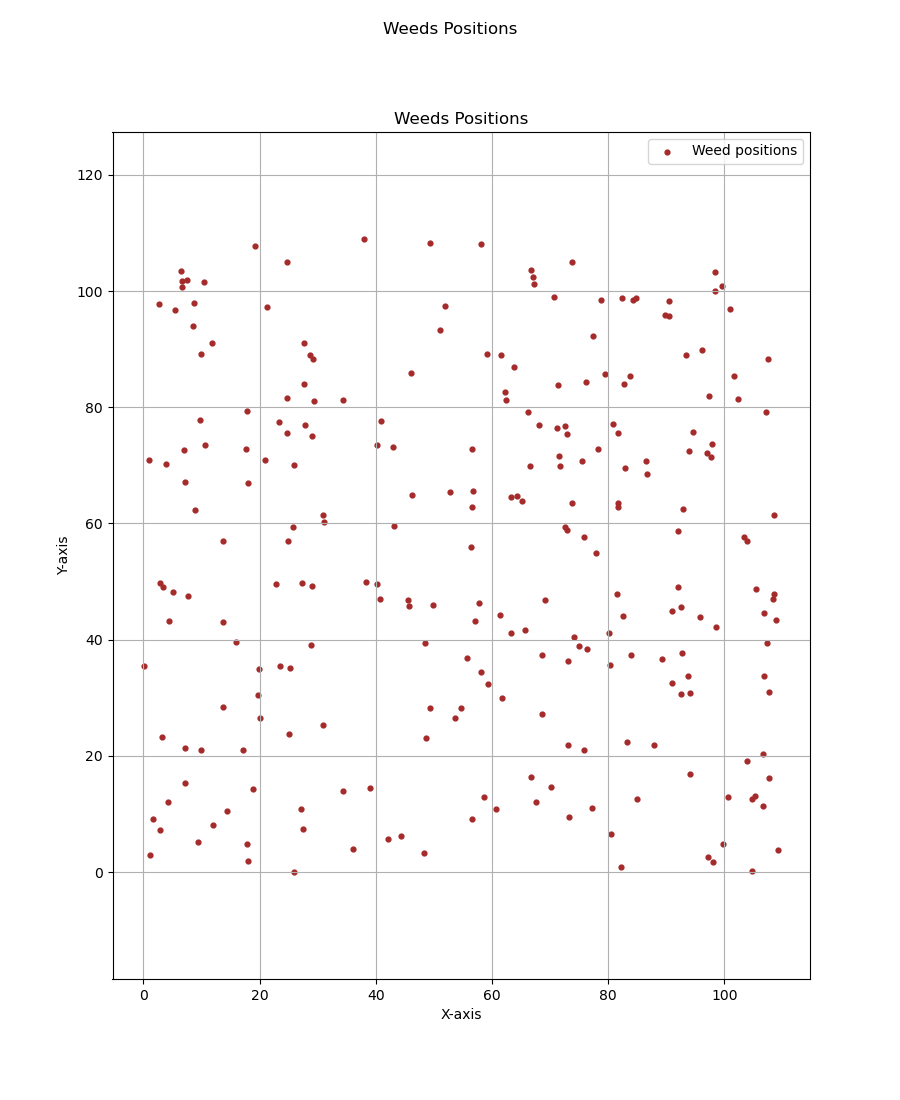
\includegraphics[height=36mm,width=0.24\textwidth]{Images/data/01.png}
        & 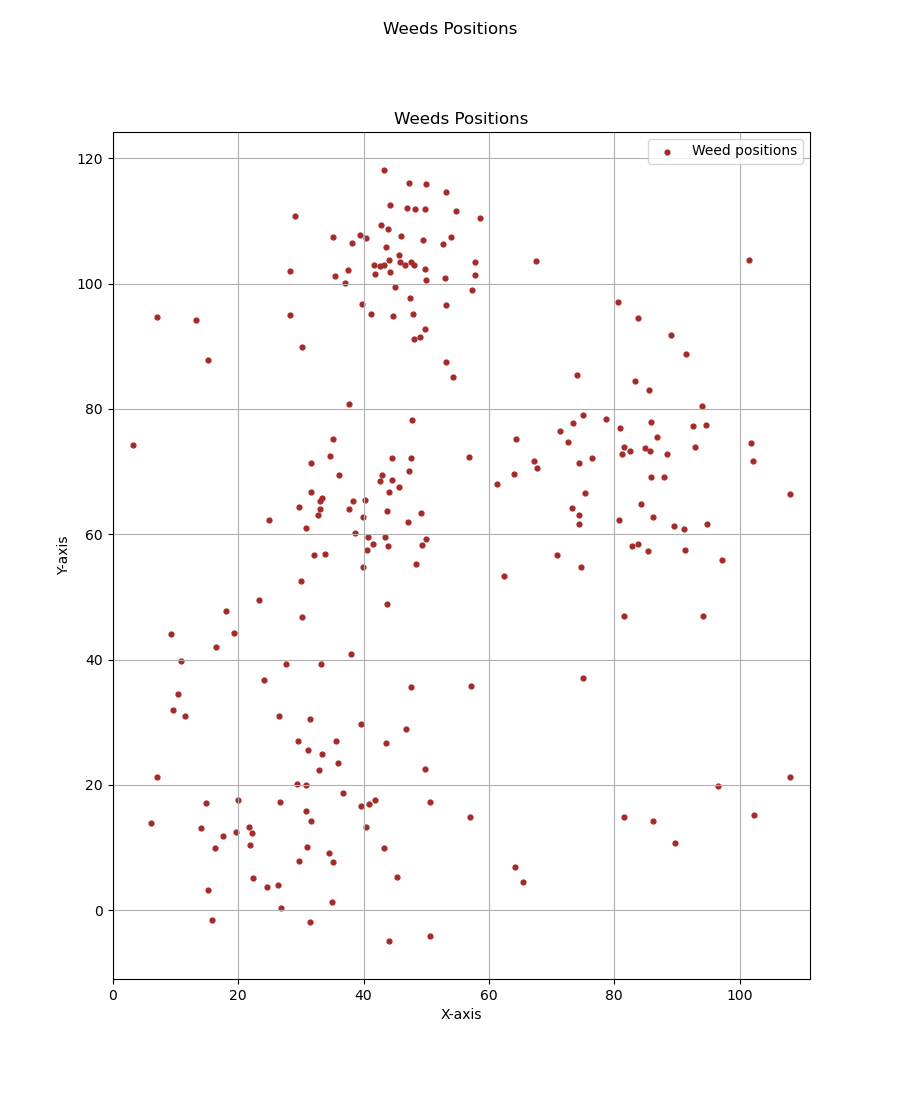
\includegraphics[height=36mm,width=0.24\textwidth]{Images/data/02.png}
        & 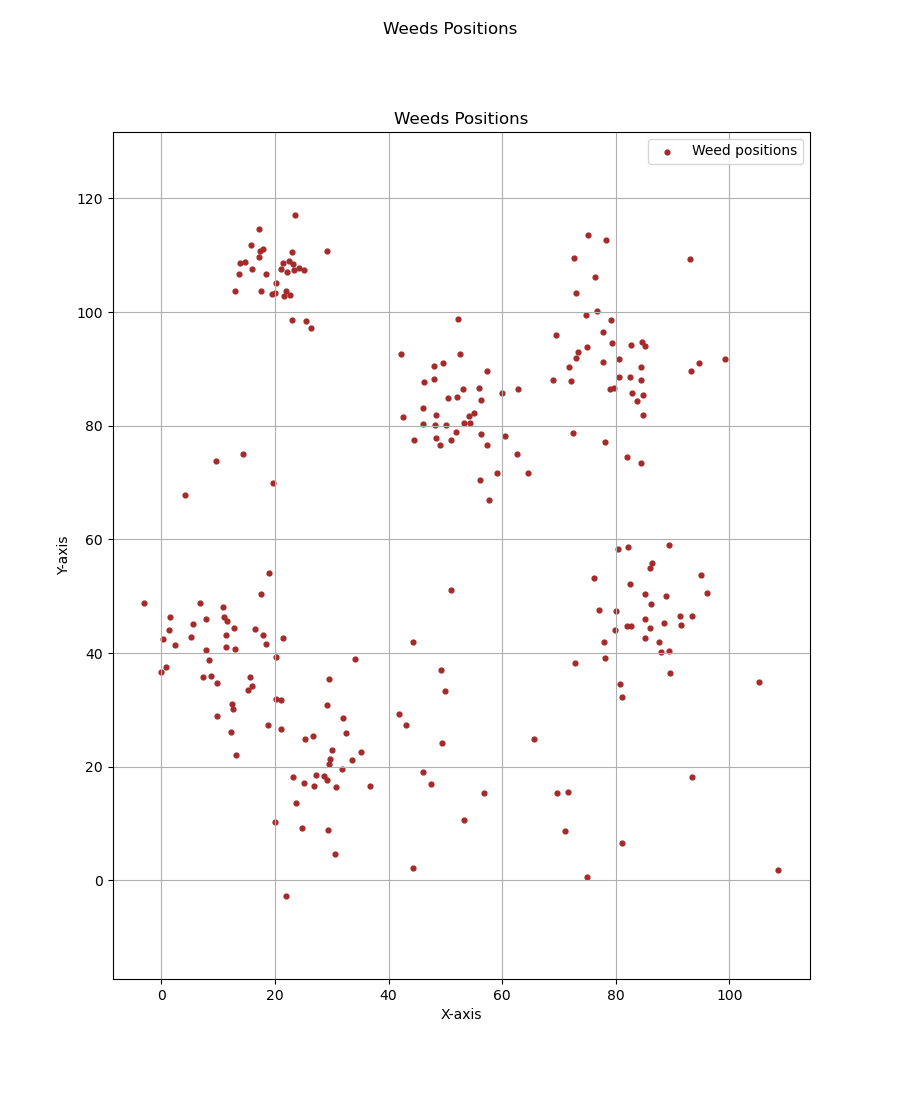
\includegraphics[height=36mm,width=0.24\textwidth]{Images/data/03.png}
         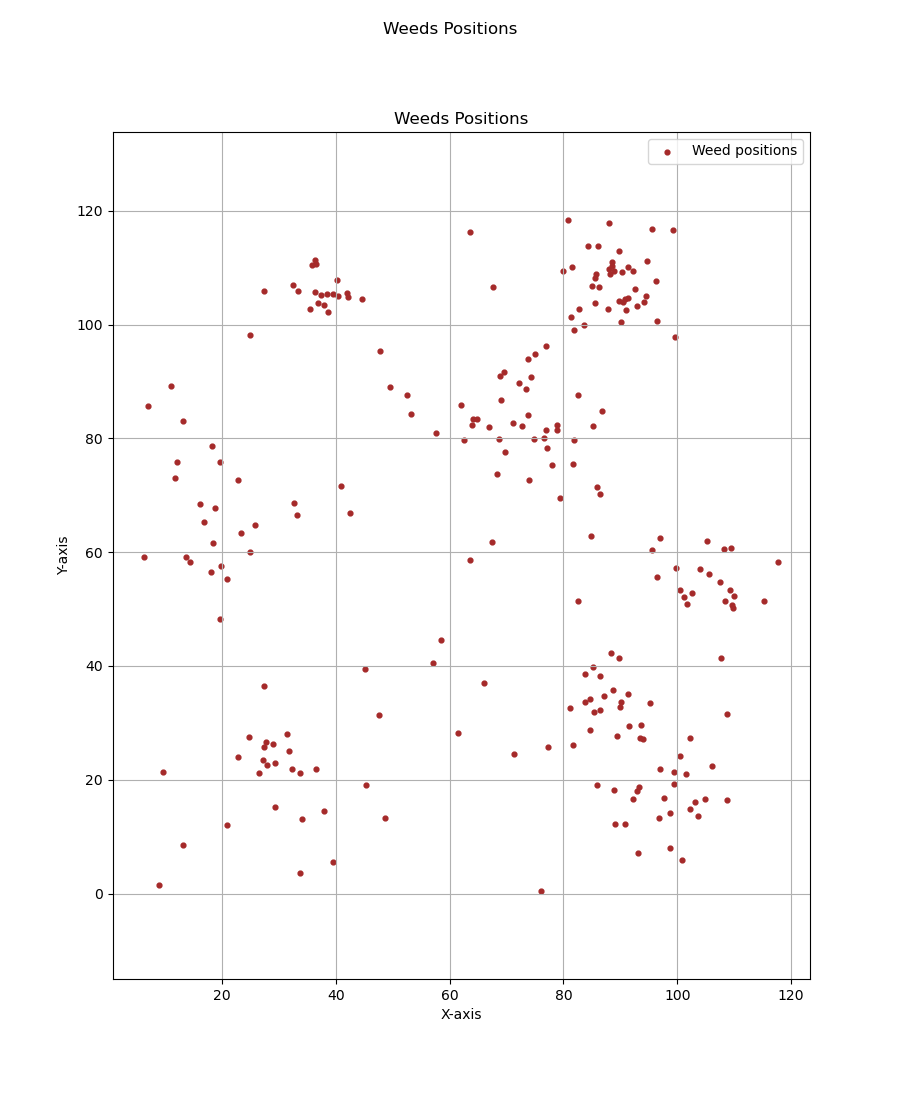
\includegraphics[height=36mm,width=0.24\textwidth]{Images/data/04.png}\\[-4pt]

        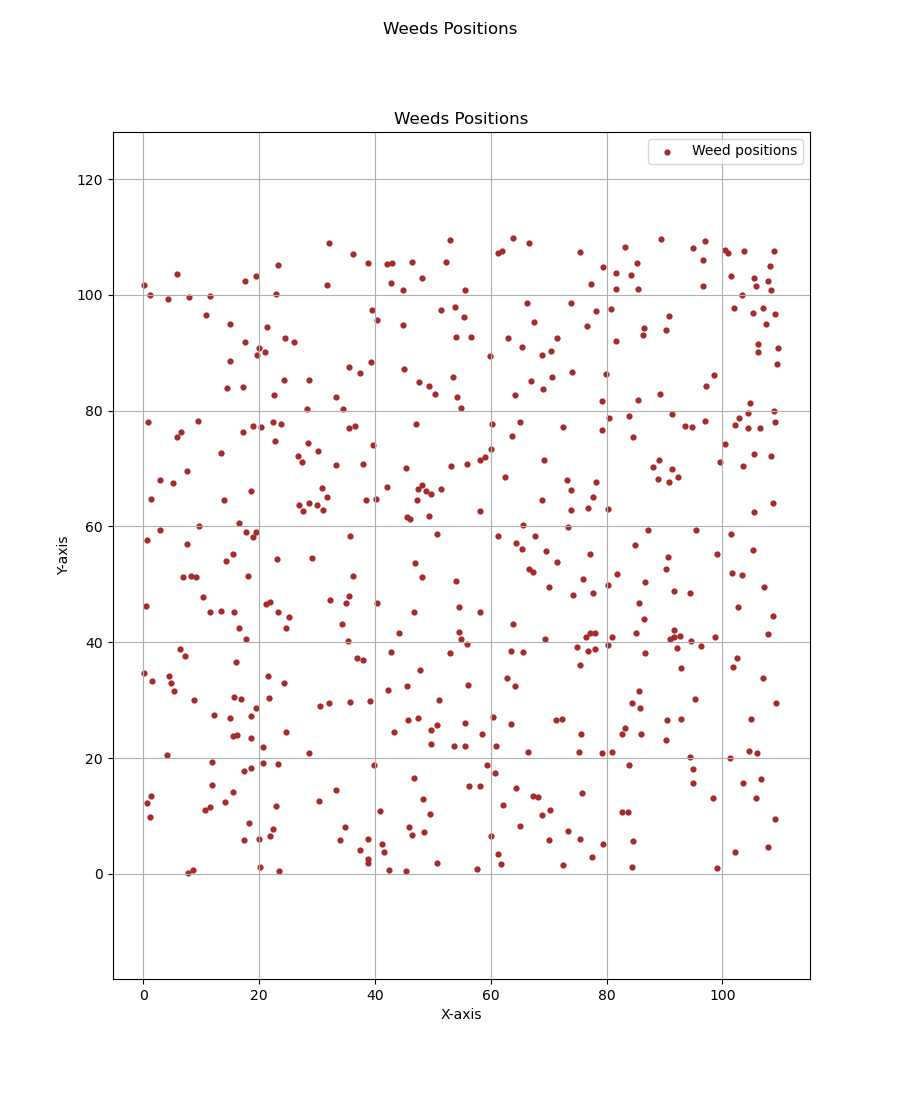
\includegraphics[height=36mm,width=0.24\textwidth]{Images/data/11.png}
        & 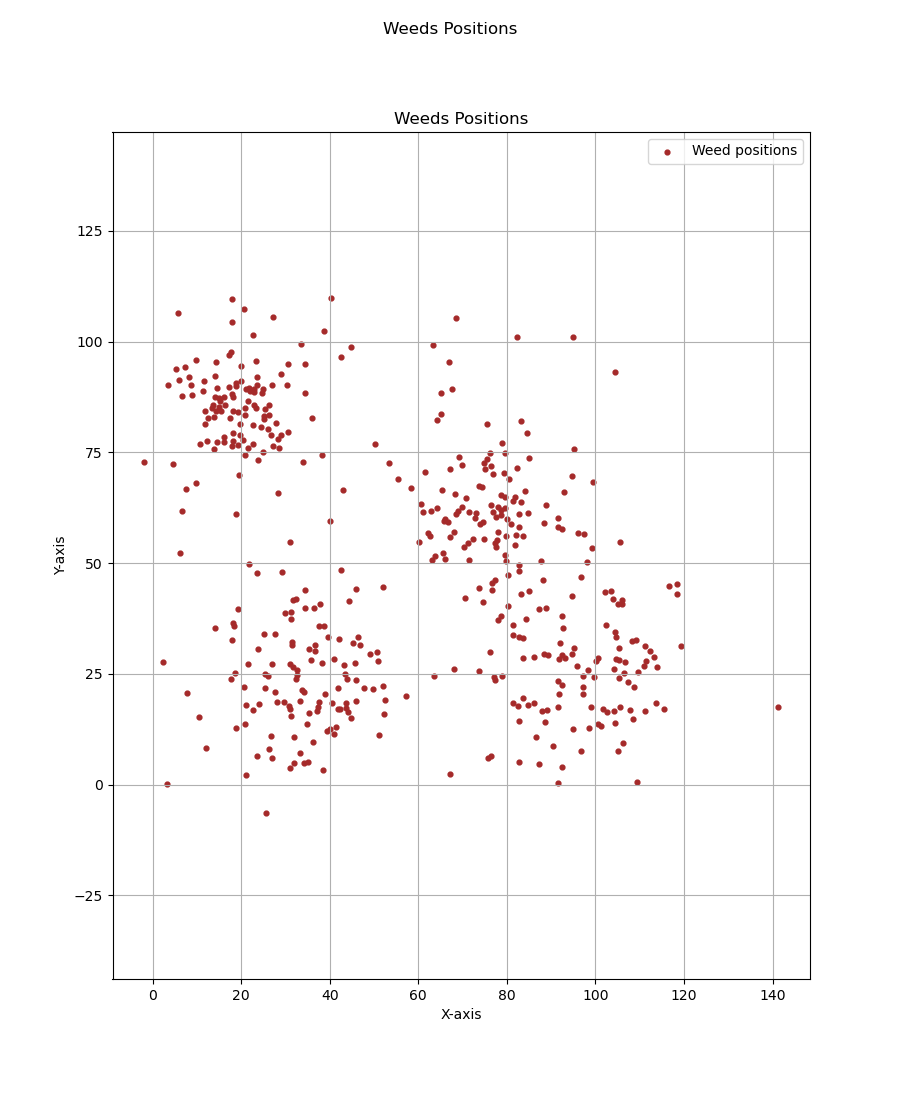
\includegraphics[height=36mm,width=0.24\textwidth]{Images/data/12.png}
        & 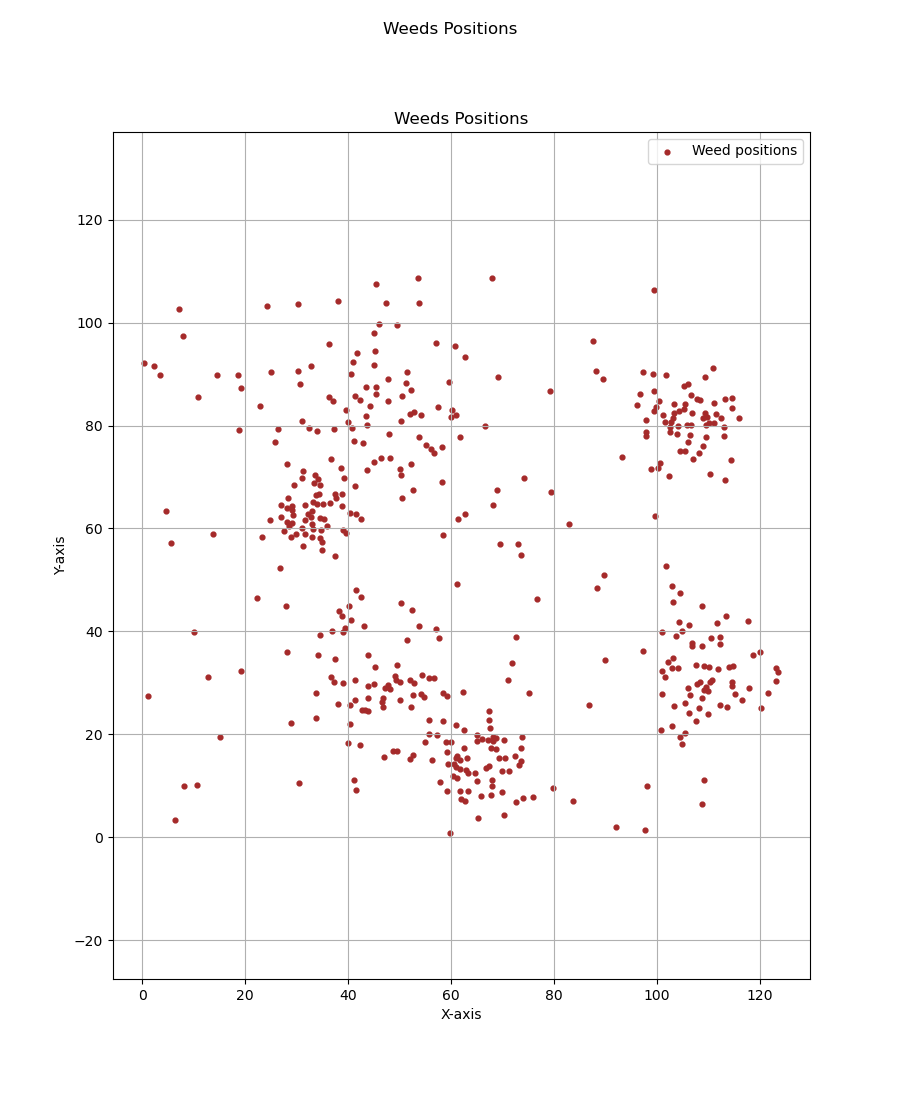
\includegraphics[height=36mm,width=0.24\textwidth]{Images/data/13.png}
        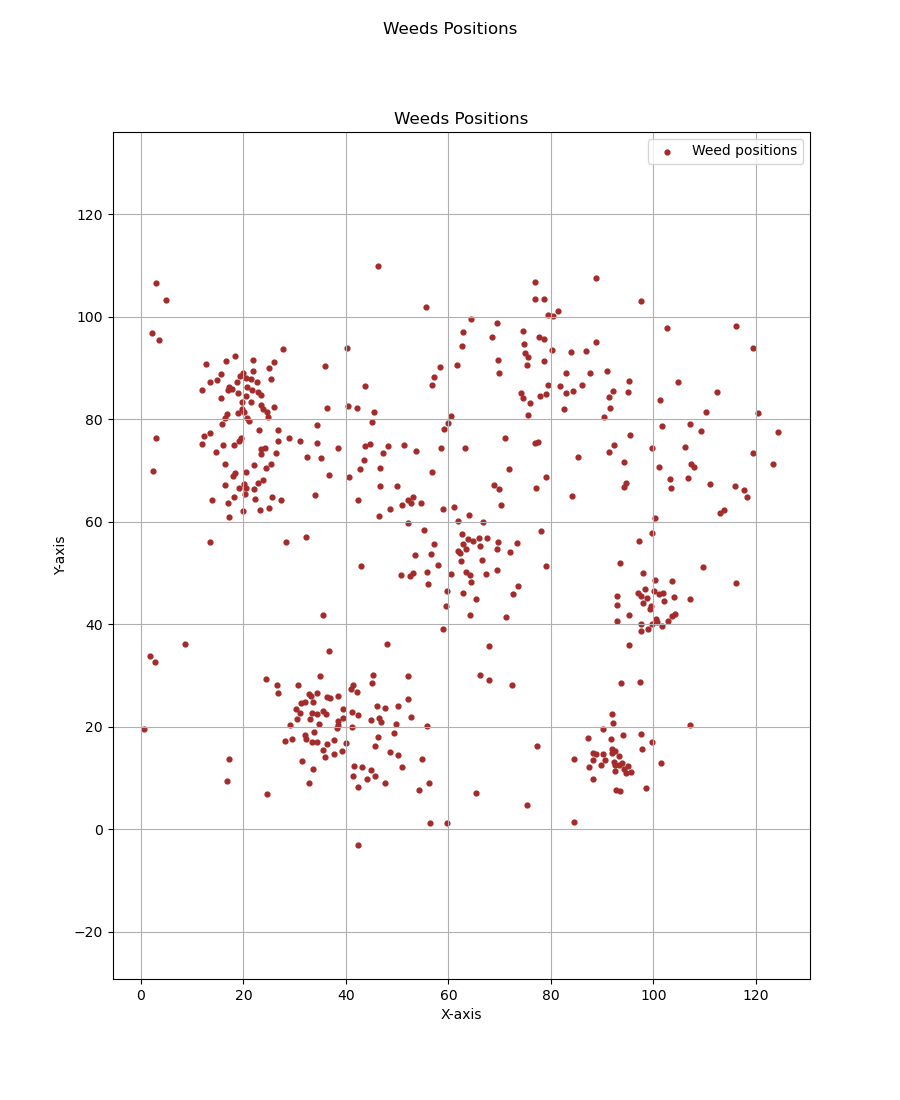
\includegraphics[height=36mm,width=0.24\textwidth]{Images/data/14.png}\\[-4pt]

        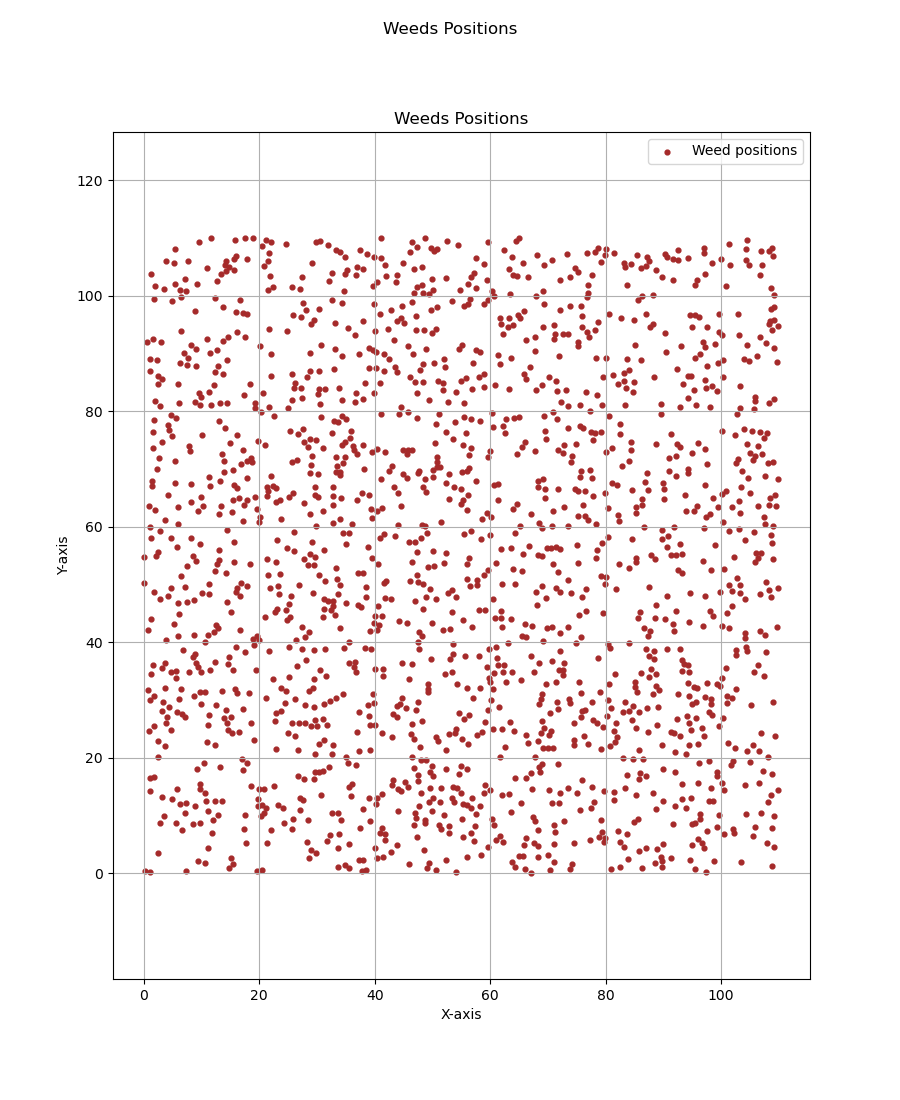
\includegraphics[height=36mm,width=0.24\textwidth]{Images/data/21.png}
        & 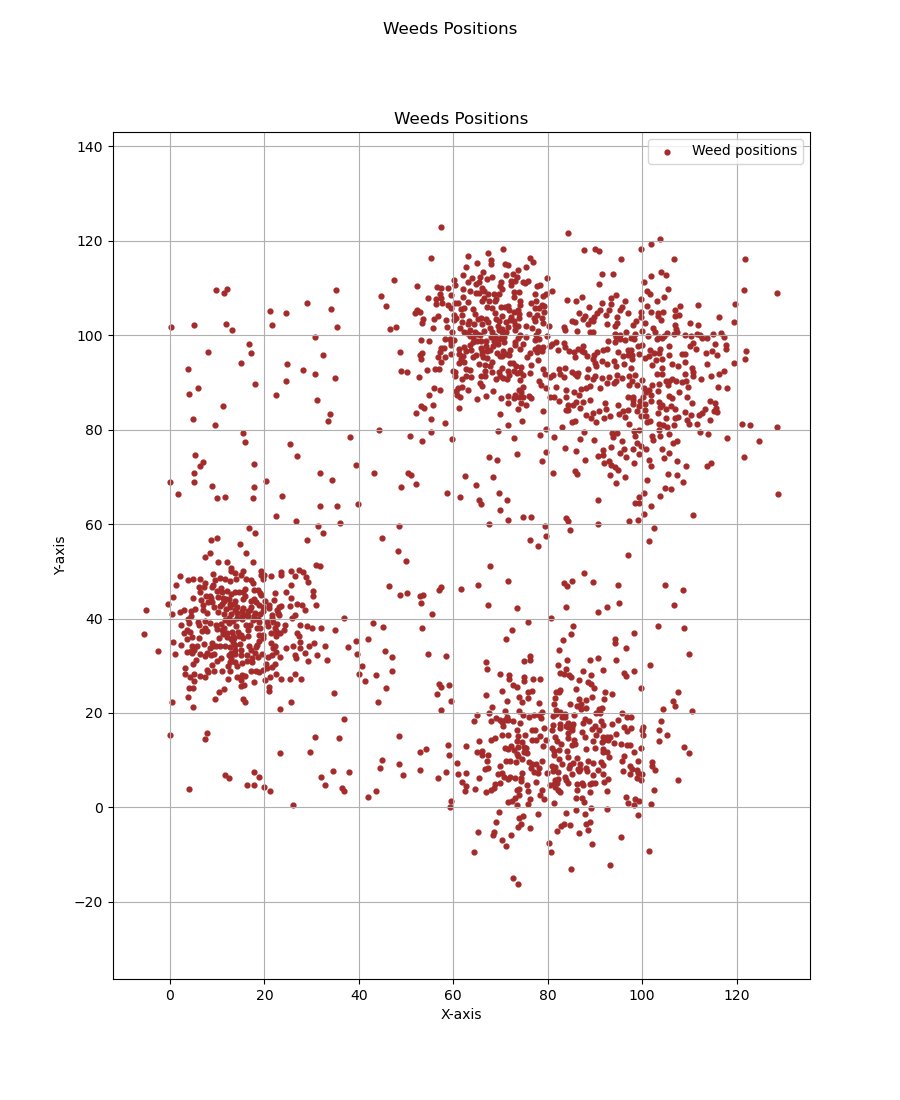
\includegraphics[height=36mm,width=0.24\textwidth]{Images/data/22.png}
        & 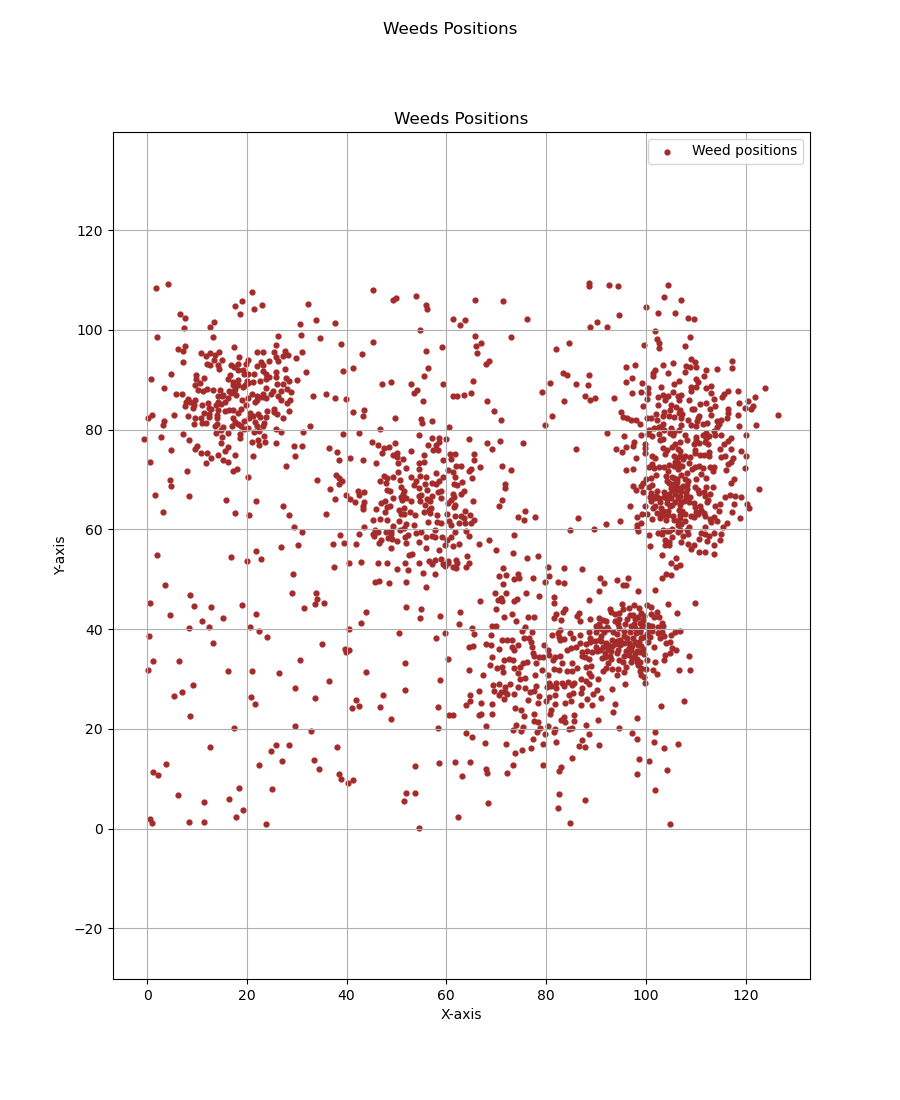
\includegraphics[height=36mm,width=0.24\textwidth]{Images/data/23.png}
         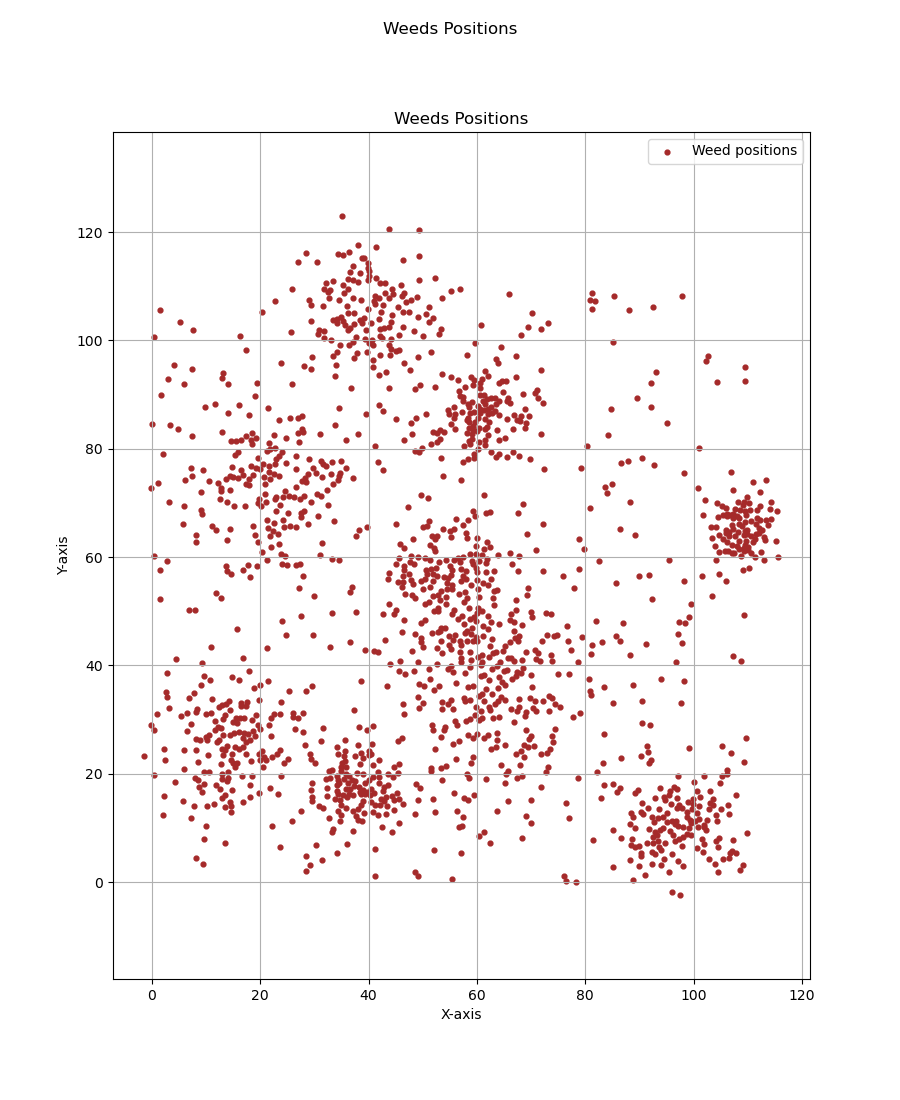
\includegraphics[height=36mm,width=0.24\textwidth]{Images/data/24.png}\\[-4pt]

         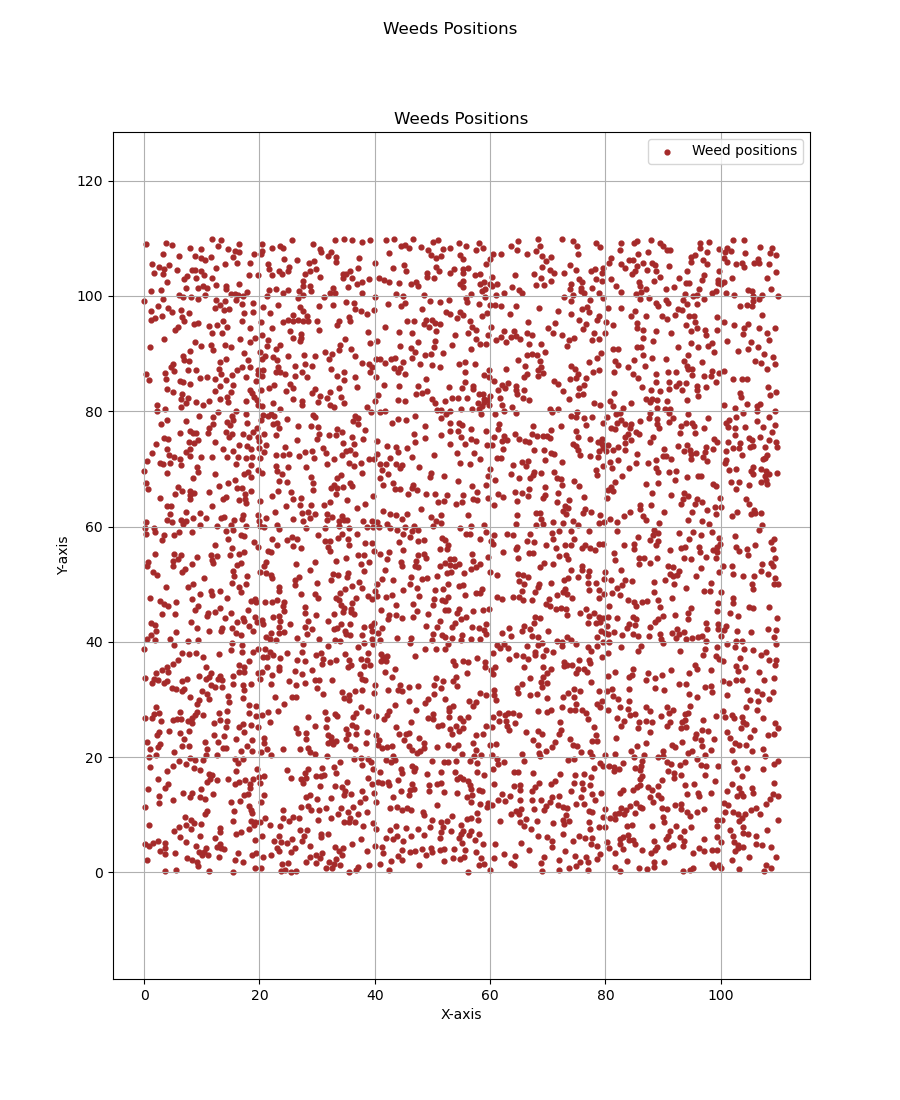
\includegraphics[height=36mm,width=0.24\textwidth]{Images/data/31.png}
        & 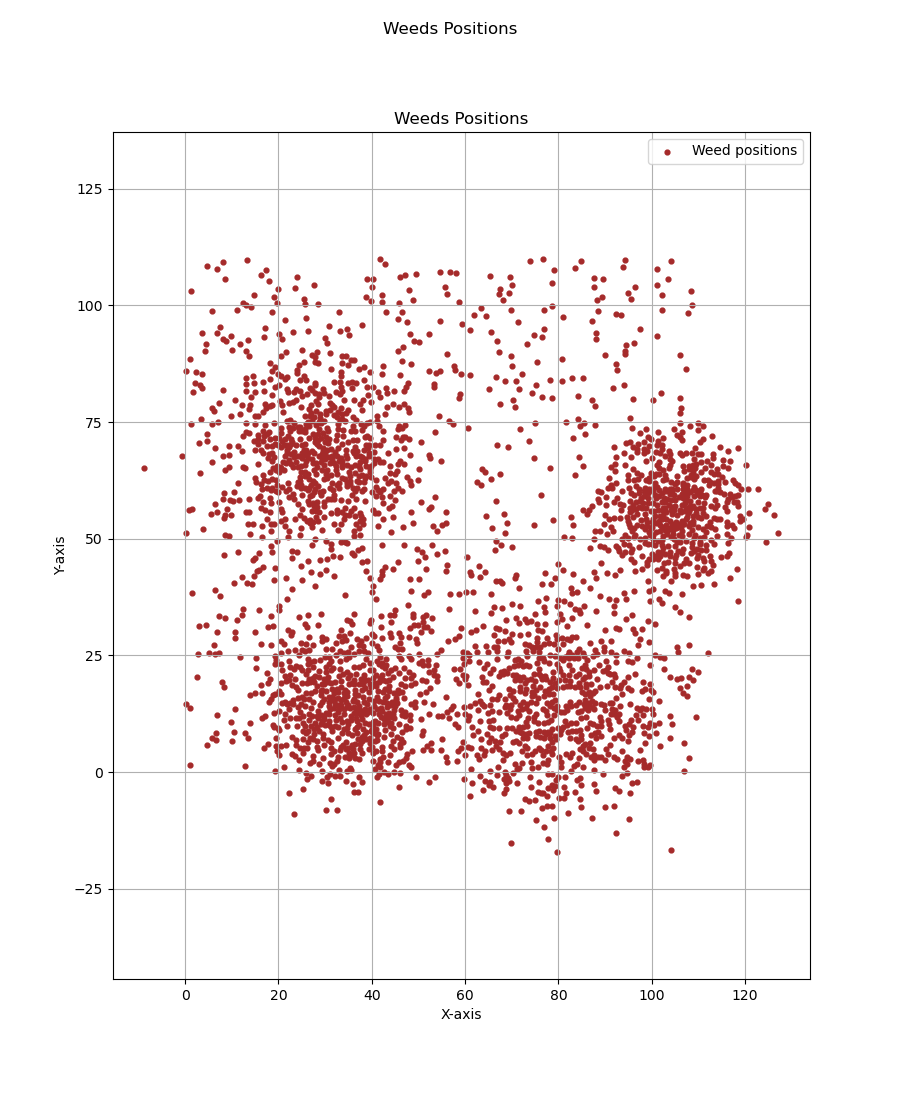
\includegraphics[height=36mm,width=0.24\textwidth]{Images/data/32.png}
        & 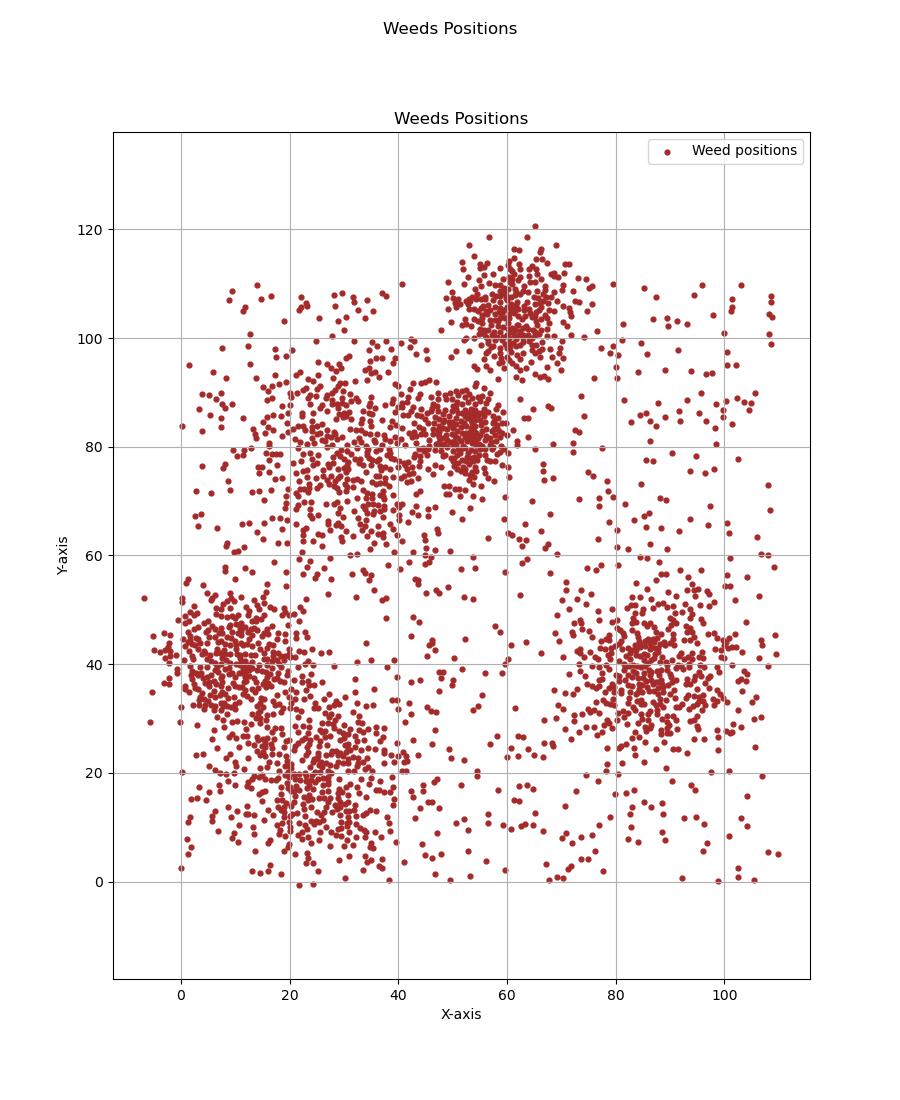
\includegraphics[height=36mm,width=0.24\textwidth]{Images/data/33.png}
         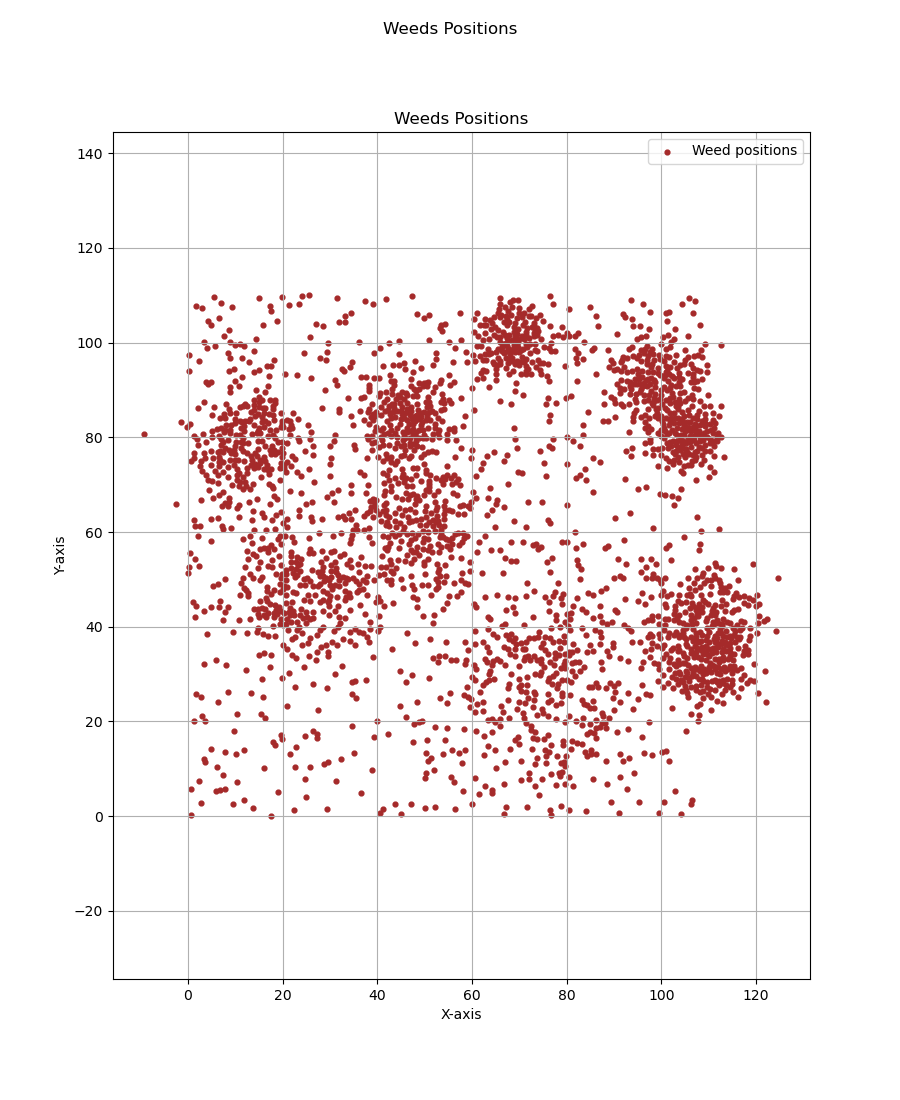
\includegraphics[height=36mm,width=0.24\textwidth]{Images/data/34.png}\\[-4pt]


        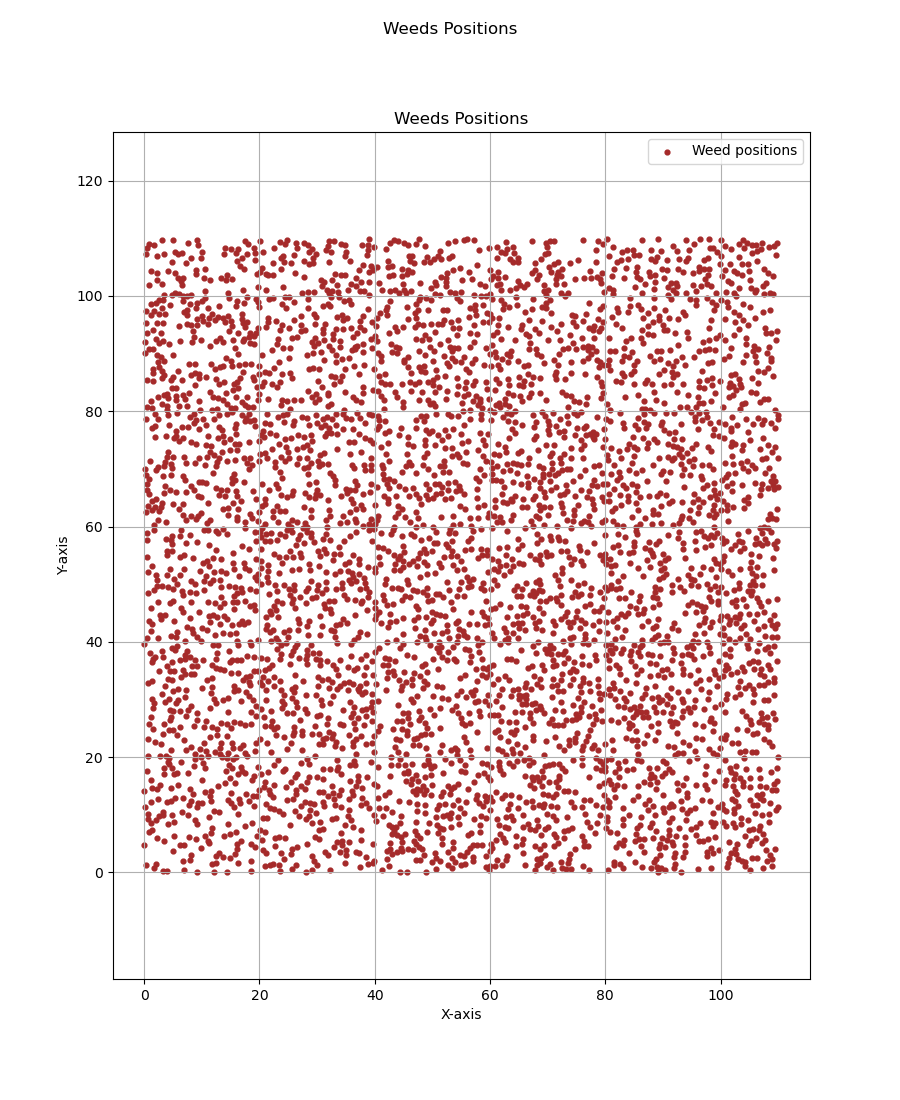
\includegraphics[height=36mm,width=0.24\textwidth]{Images/data/41.png}
        & 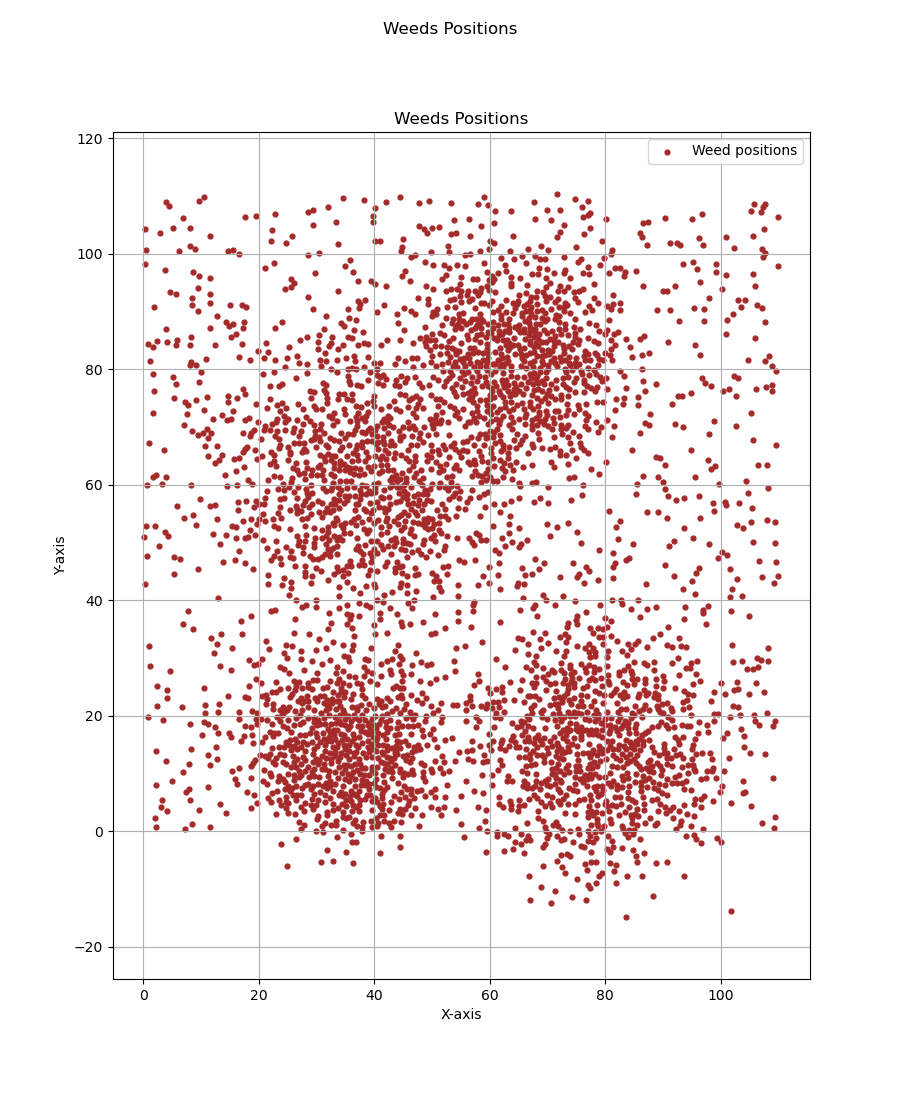
\includegraphics[height=36mm,width=0.24\textwidth]{Images/data/42.png}
        & 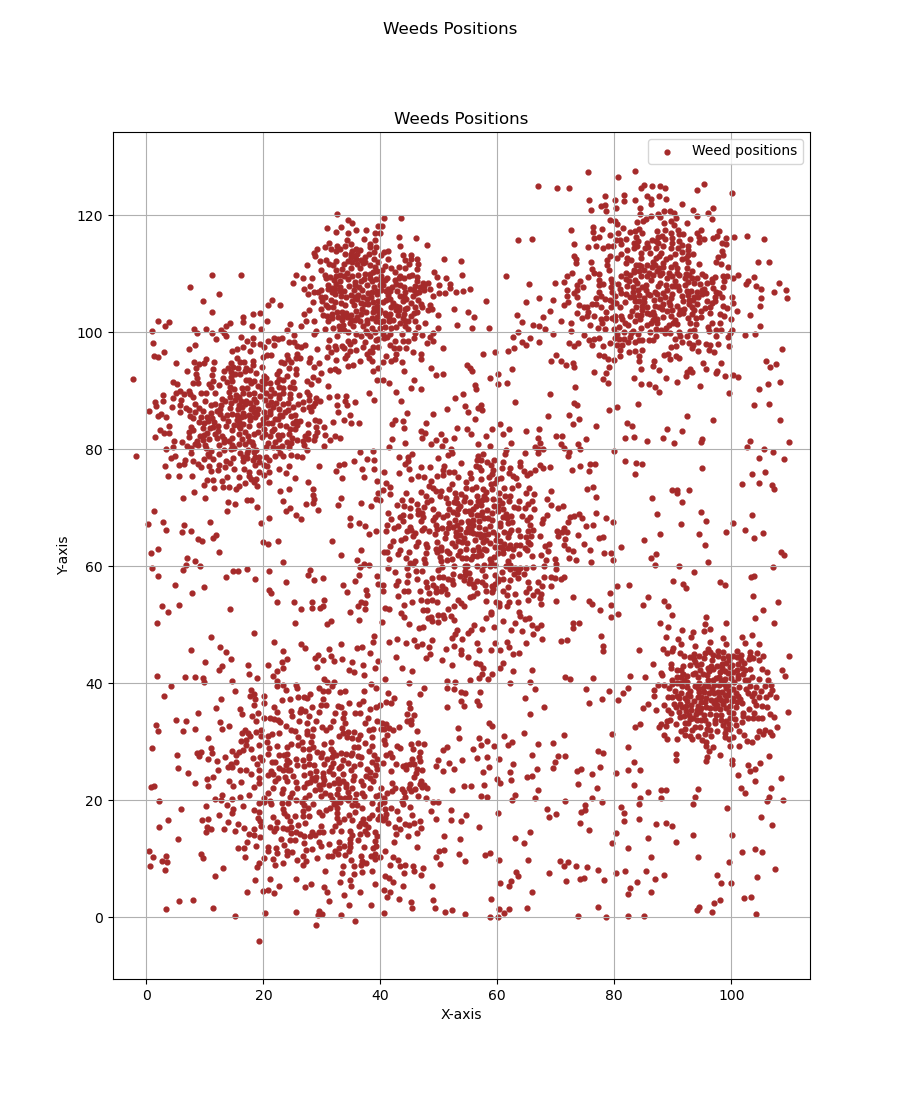
\includegraphics[height=36mm,width=0.24\textwidth]{Images/data/43.png}
        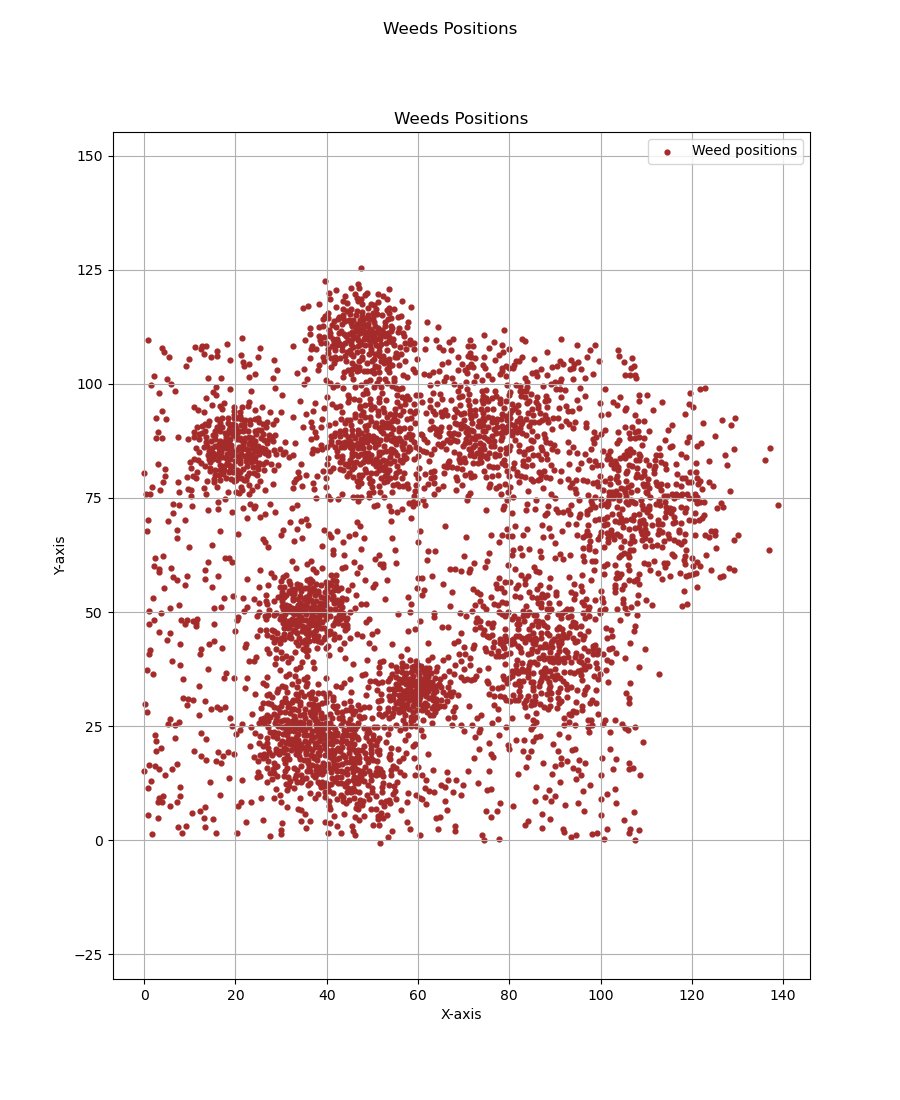
\includegraphics[height=36mm,width=0.24\textwidth]{Images/data/44.png}\\[-4pt]

        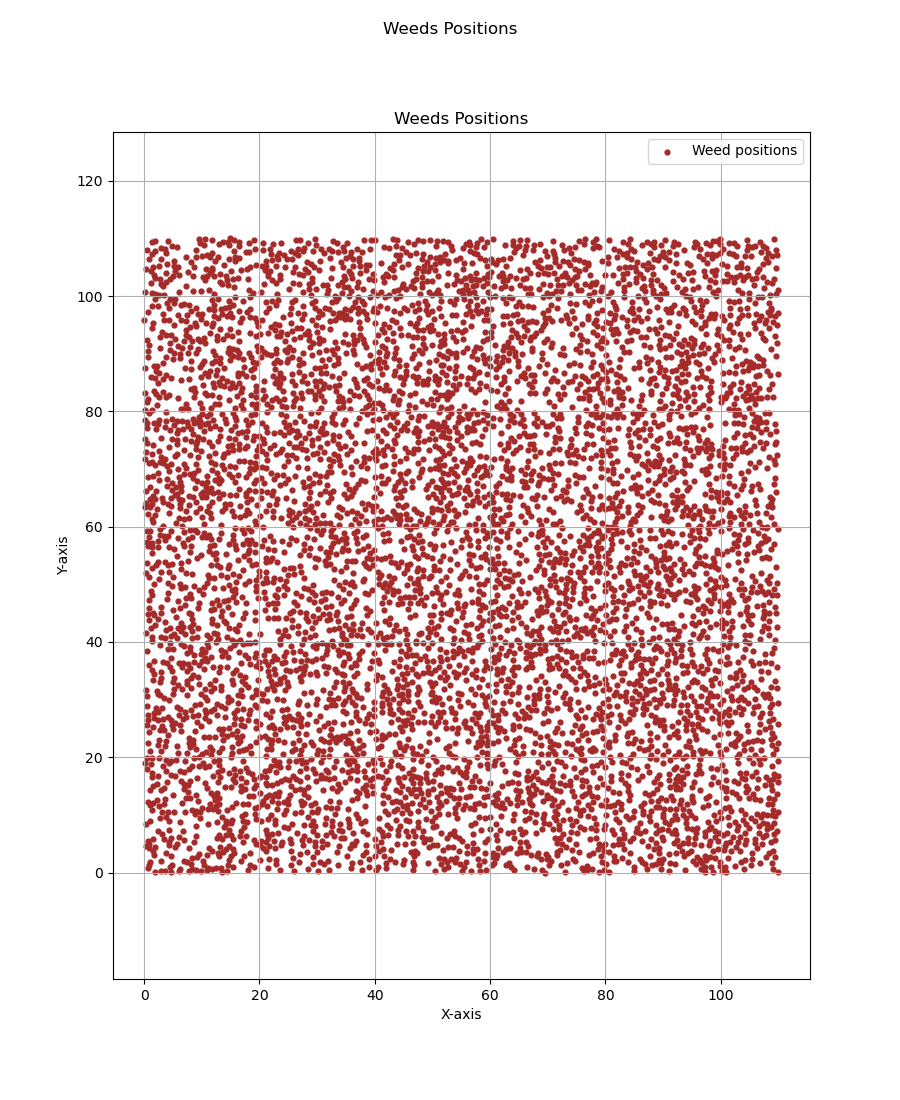
\includegraphics[height=36mm,width=0.24\textwidth]{Images/data/51.png}
        & 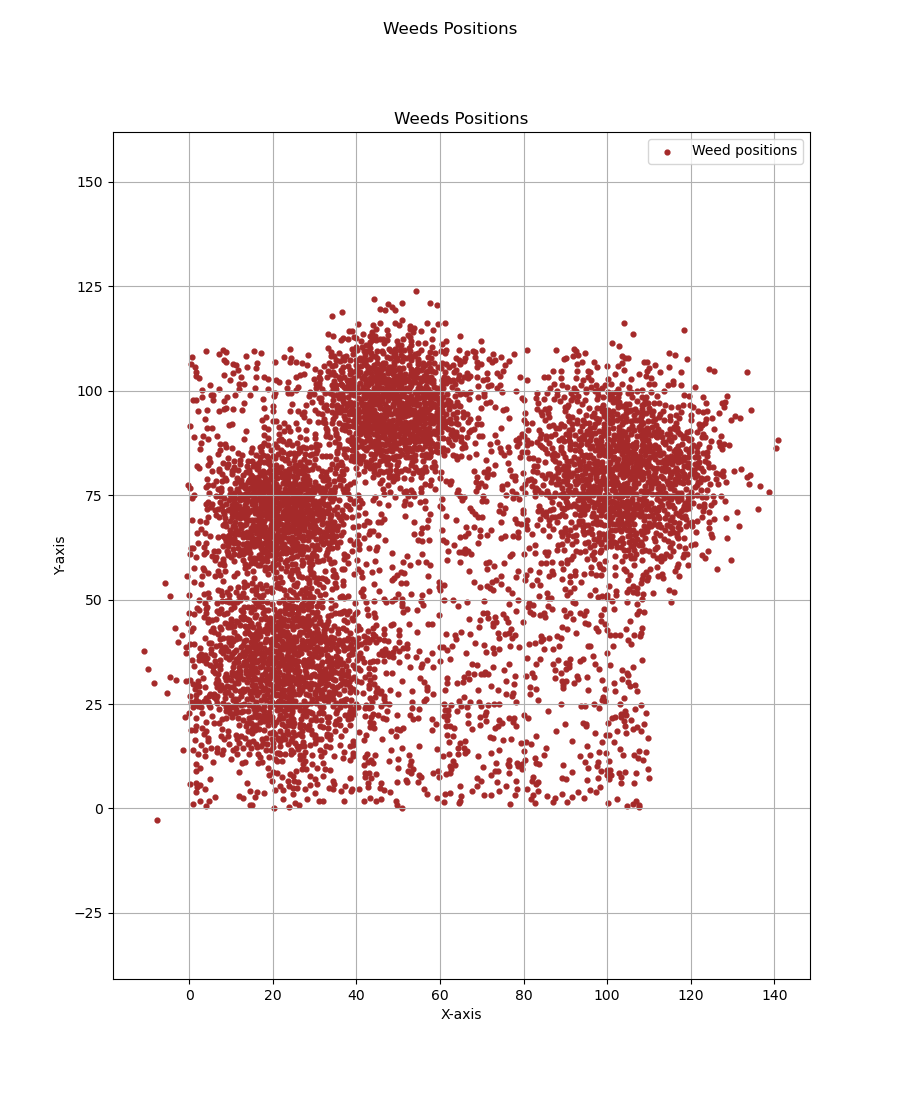
\includegraphics[height=36mm,width=0.24\textwidth]{Images/data/52.png}
        & 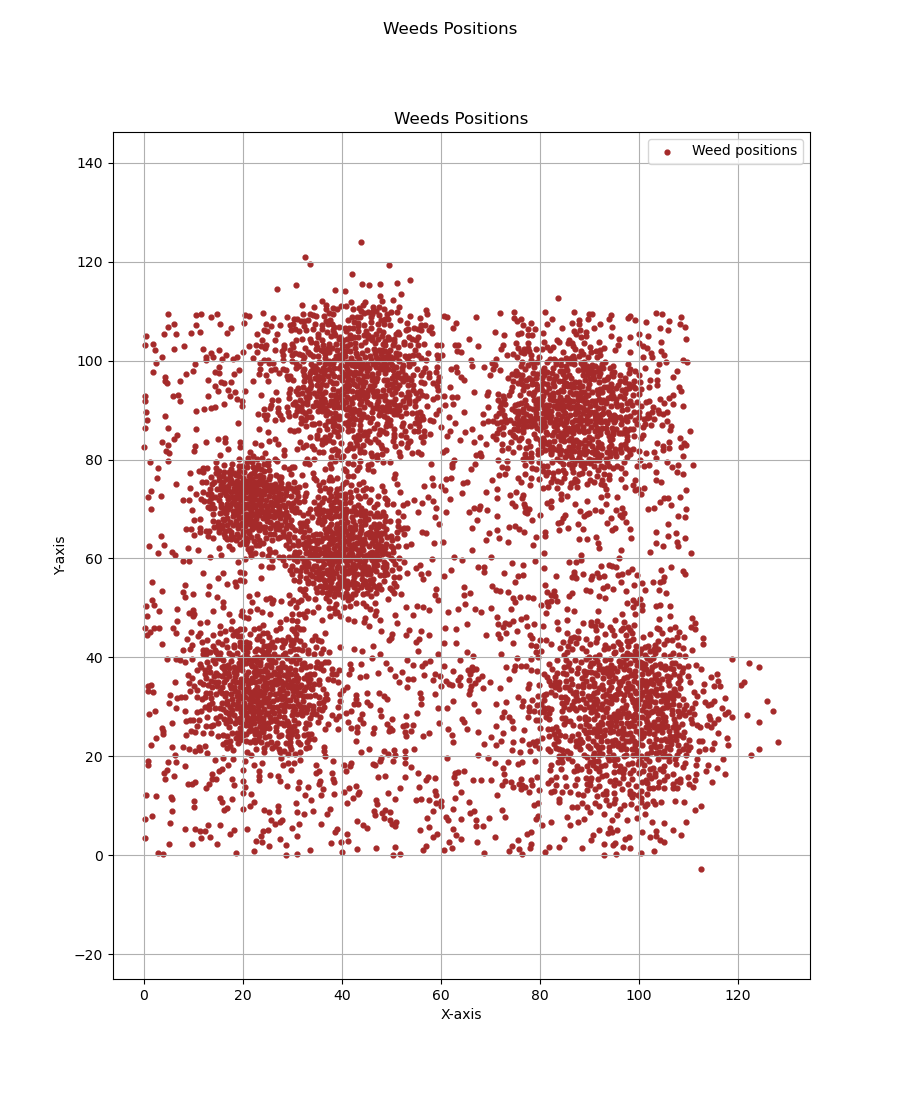
\includegraphics[height=36mm,width=0.24\textwidth]{Images/data/53.png}
        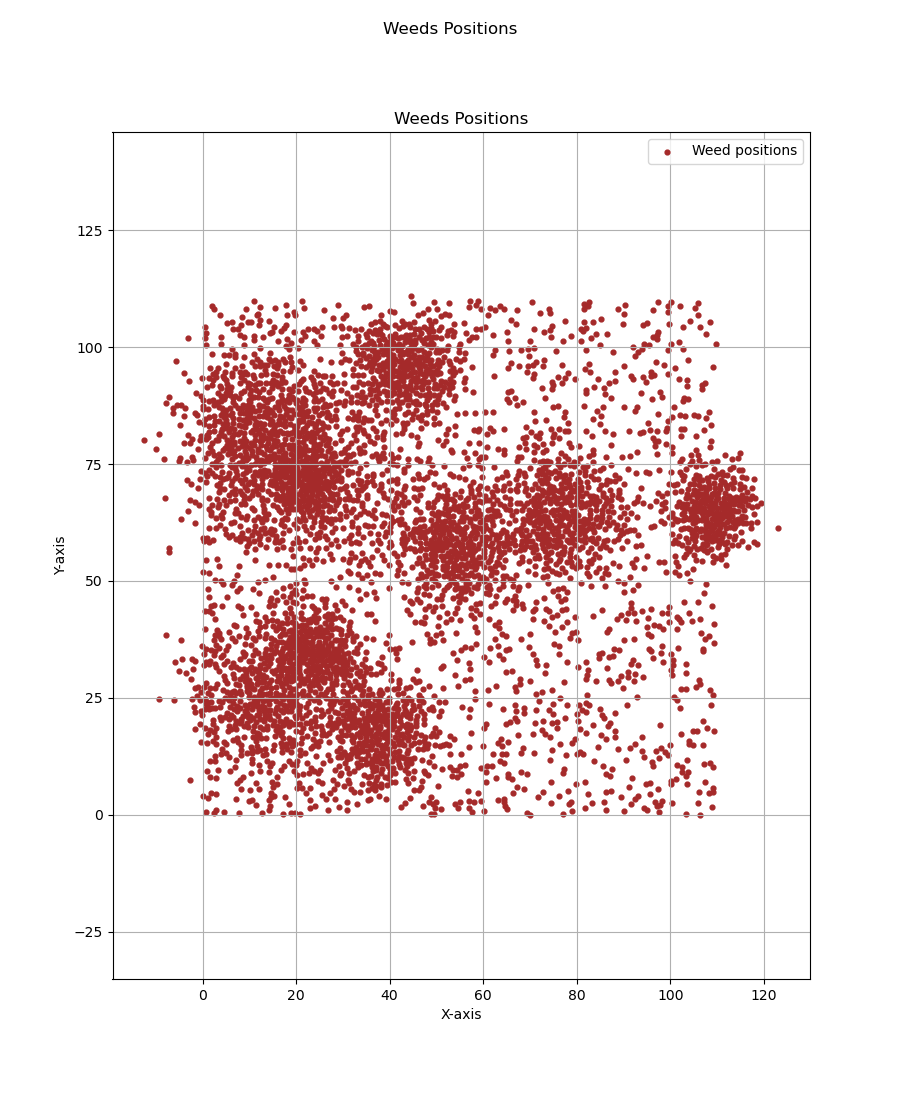
\includegraphics[height=36mm,width=0.24\textwidth]{Images/data/54.png}\\[-4pt]
        
    \end{tabular}
    \caption{Dataset.\label{fig:Dataset}}
\end{figure}


\section{Simulation Results and Analysis}

This section presents the detailed results and analysis of the simulation experiments conducted to evaluate the robustness of the proposed complete coverage path planning behavioral algorithm. The empirical findings are meticulously analyzed to provide insights into the algorithm's performance under diverse scenarios, enabling a comprehensive assessment of its efficiency and effectiveness. 

\vspace{3mm}  

\textbf{Experimental Consistency}
To ensure the validity of comparisons and isolate the effects of different datasets on the algorithm's performance, the initial position and orientation of the robot were kept constant throughout all experiments. Additionally, the parameters for both the robot and the algorithm were consistently maintained across all trials.


\vspace{3mm}  

\textbf{Robot Constraints and Algorithm Parameters: } 


The robot's constraints and operational parameters are set to realistic values to ensure the validity of the simulation results. The parameters' data can be visualized in (\autoref{tab:constraints_and_parameters_1}), offering a comprehensive overview of the robot's physical and operational characteristics.

% % % % % Table robot parameters 1
\begin{table}[H] 
    \centering
    \caption{Robot and algorithm Constraints and Parameters}
    \label{tab:constraints_and_parameters_1}
    \begin{tabular}{|c|c|}
    \hline
    \rowcolor[HTML]{FFCC67} 
    \textit{\textbf{Constraints and Parameters}}                                    & \textit{\textbf{Values}} \\ \hline
    \rowcolor[HTML]{BBF6F4} 
    \textit{Robot initial position}                                                 & {[}60.0, 1.0{]}          \\ \hline
    \rowcolor[HTML]{BBF6F4} 
    \textit{Robot initial orientation}                                              & 120                      \\ \hline
    \rowcolor[HTML]{BBF6F4} 
    \textit{Search angle of the vision cone}                                        & ±11                      \\ \hline
    \rowcolor[HTML]{BBF6F4} 
    \textit{Minimum search radius of the vision cone.}                              & 1.25                     \\ \hline
    \rowcolor[HTML]{BBF6F4} 
    \textit{Maximum search radius of the vision cone.}                              & 100                      \\ \hline
    \rowcolor[HTML]{BBF6F4} 
    \textit{Minimum turning radius allowed for the robot.}                          & 2.0                      \\ \hline
    \rowcolor[HTML]{BBF6F4} 
    \textit{robot velocity on curved paths.}                                        & 0.4                      \\ \hline
    \rowcolor[HTML]{BBF6F4} 
    \textit{robot velocity on straight paths.}                                      & 0.8                      \\ \hline
    \rowcolor[HTML]{BBF6F4} 
    \textit{Distance used to compute field time taken on curved paths.}             & 7.85                     \\ \hline
    \rowcolor[HTML]{BBF6F4} 
    \textit{Number of points to consider in the vision cone.}                       & 5                        \\ \hline
    \rowcolor[HTML]{BEF7F5} 
    \textit{Minimum distance between intermediate points, and start and end point.} & 2.7                      \\ \hline
    \rowcolor[HTML]{BEF7F5} 
    \textit{Minimum distance between intermediate points.}                          & 2                        \\ \hline
    \rowcolor[HTML]{BEF7F5} 
    \textit{Maximum distance of the point form the path.}                           & 0.6                      \\ \hline
    \end{tabular}
    \end{table}



\vspace{3mm}   







The algorithm parameters are also meticulously defined to ensure consistent performance across all experiments. These parameters are set based on the robot's physical constraints and operational requirements, ensuring that the algorithm operates within realistic boundaries.

\vspace{3mm}

The algorithm was designed to initially compute the global coverage path using straight lines. Subsequently, Dubins paths are generated for each line segment to ensure the shortest feasible path between each pair of points, optimizing the overall path length. The (\autoref{fig:straight_path}) illustrate the straight paths generated by the algorithm for different datasets.

% Straight_path
\begin{figure}[p]
    \centering
    \begin{tabular}{ccc}
         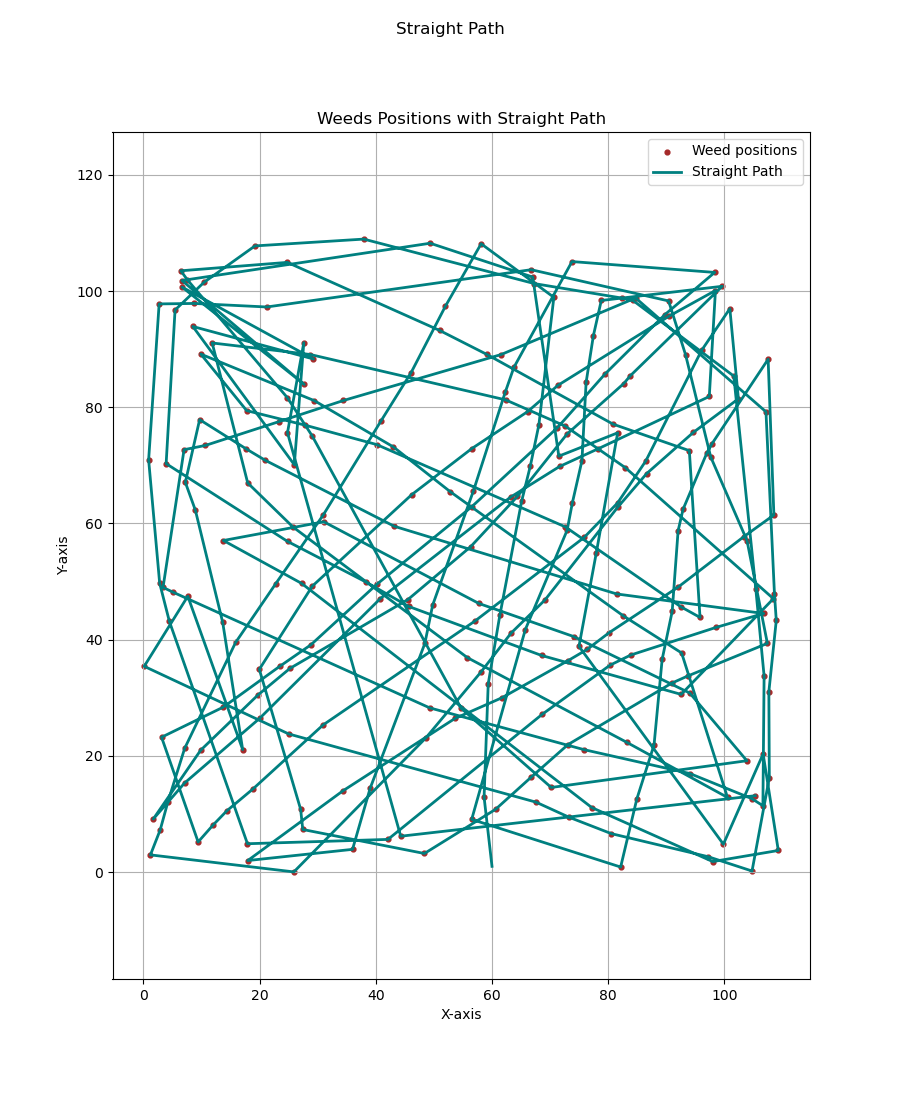
\includegraphics[height=36mm,width=0.24\textwidth]{Images/simulation_no_obs/straight_paths/01.png}
        & 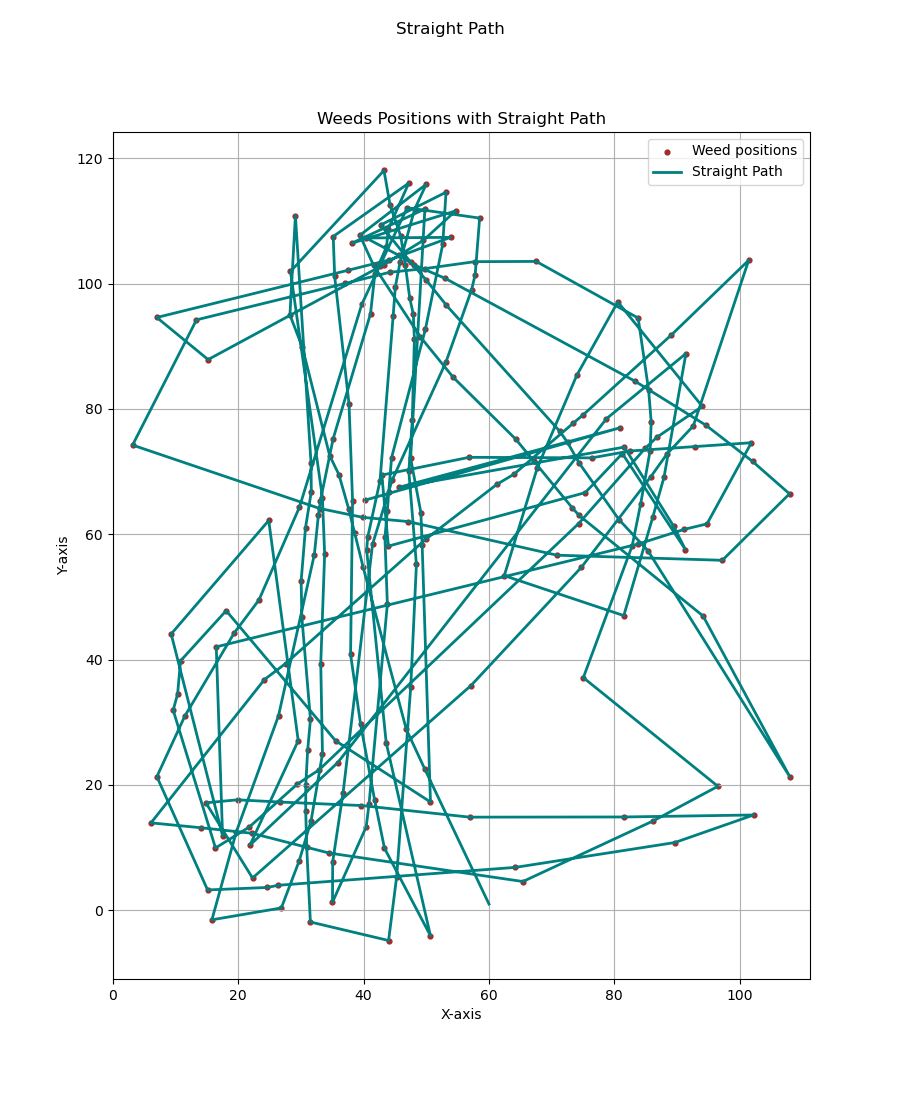
\includegraphics[height=36mm,width=0.24\textwidth]{Images/simulation_no_obs/straight_paths/02.png}
        & 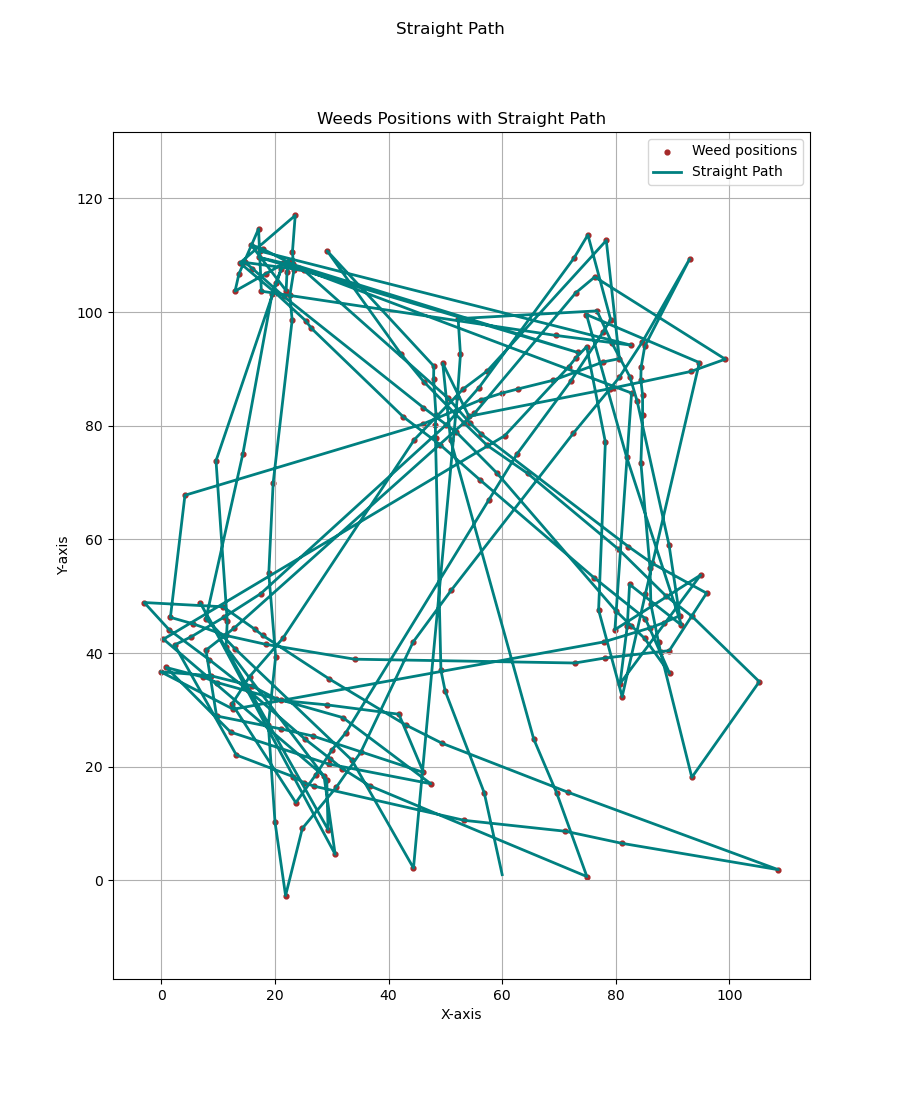
\includegraphics[height=36mm,width=0.24\textwidth]{Images/simulation_no_obs/straight_paths/03.png}
         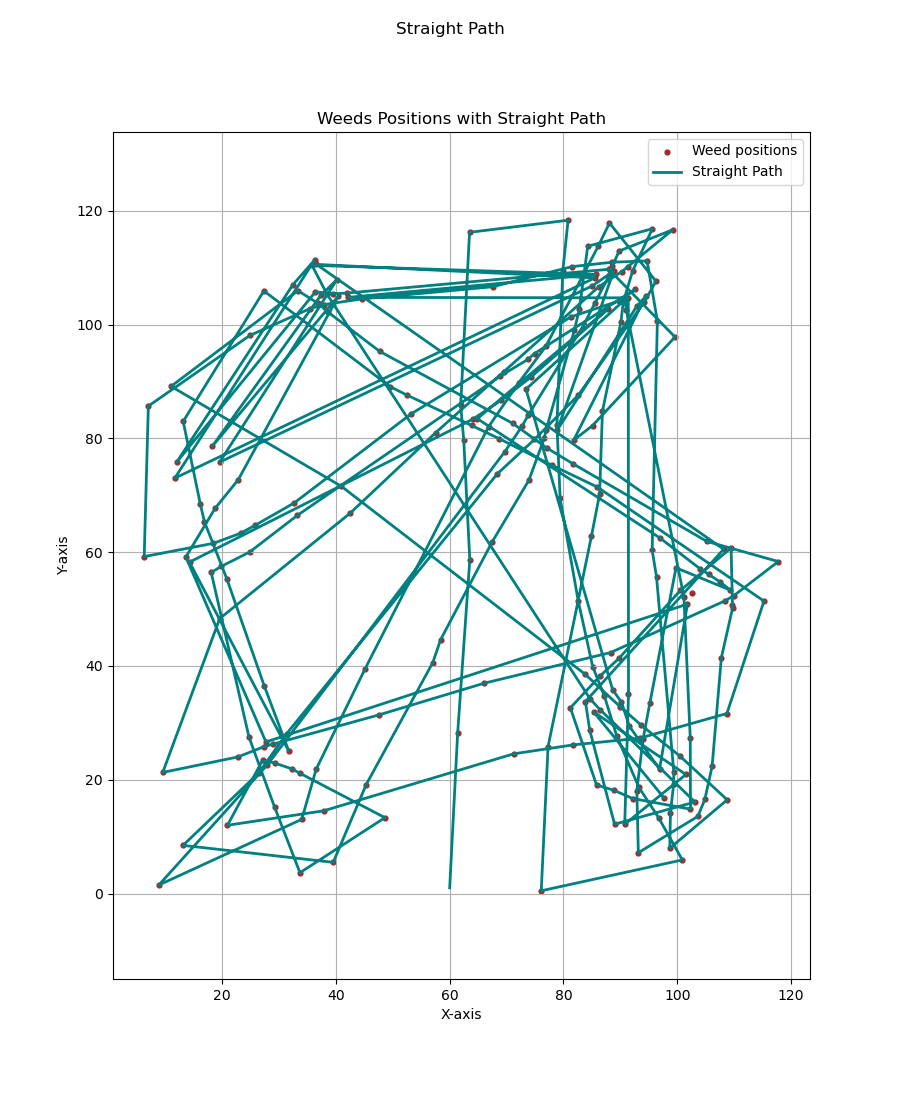
\includegraphics[height=36mm,width=0.24\textwidth]{Images/simulation_no_obs/straight_paths/04.png}\\[-4pt]

        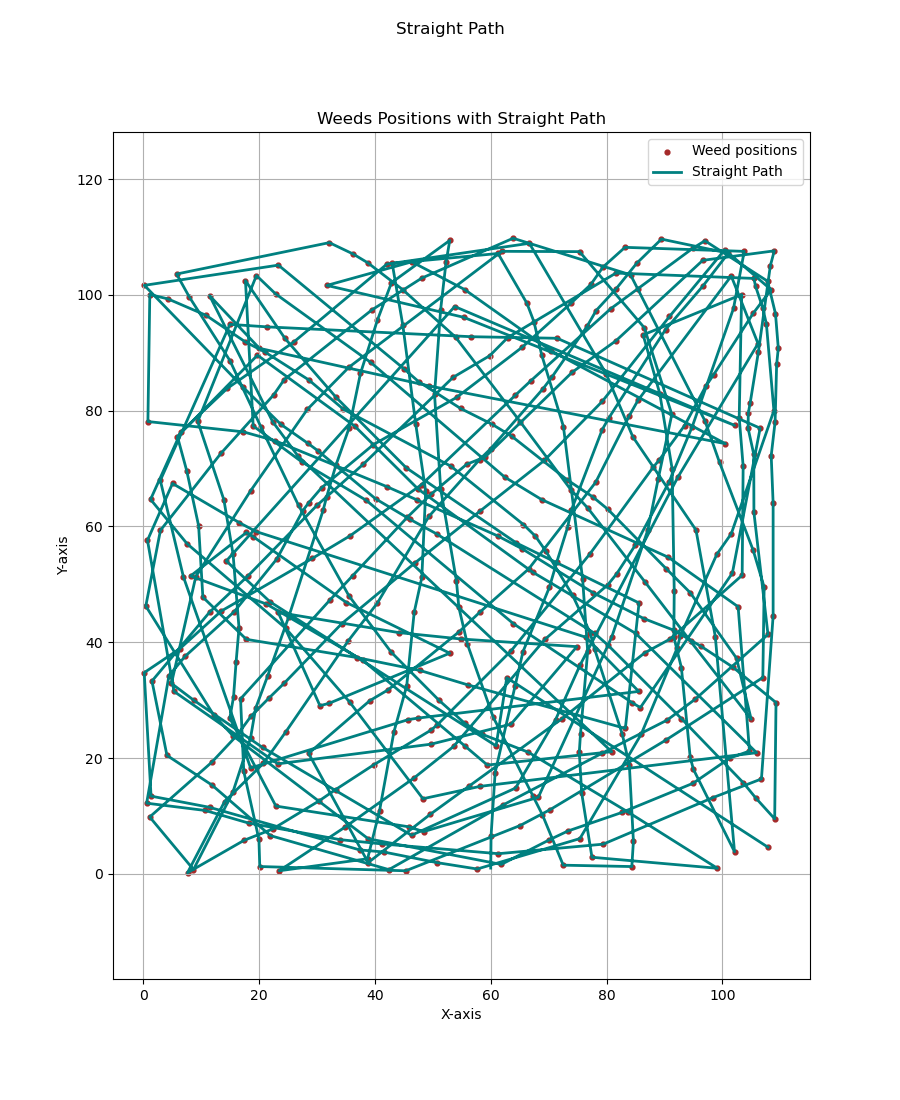
\includegraphics[height=36mm,width=0.24\textwidth]{Images/simulation_no_obs/straight_paths/11.png}
        & 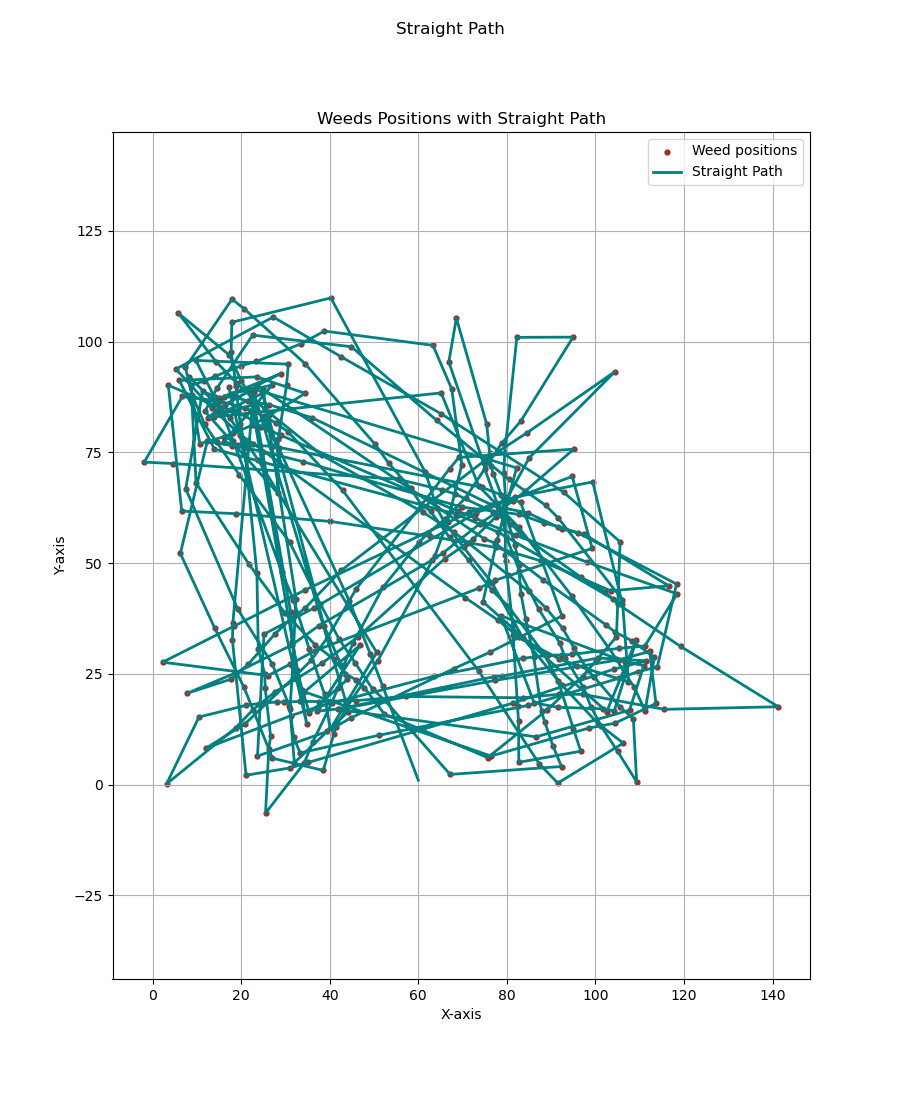
\includegraphics[height=36mm,width=0.24\textwidth]{Images/simulation_no_obs/straight_paths/12.png}
        & 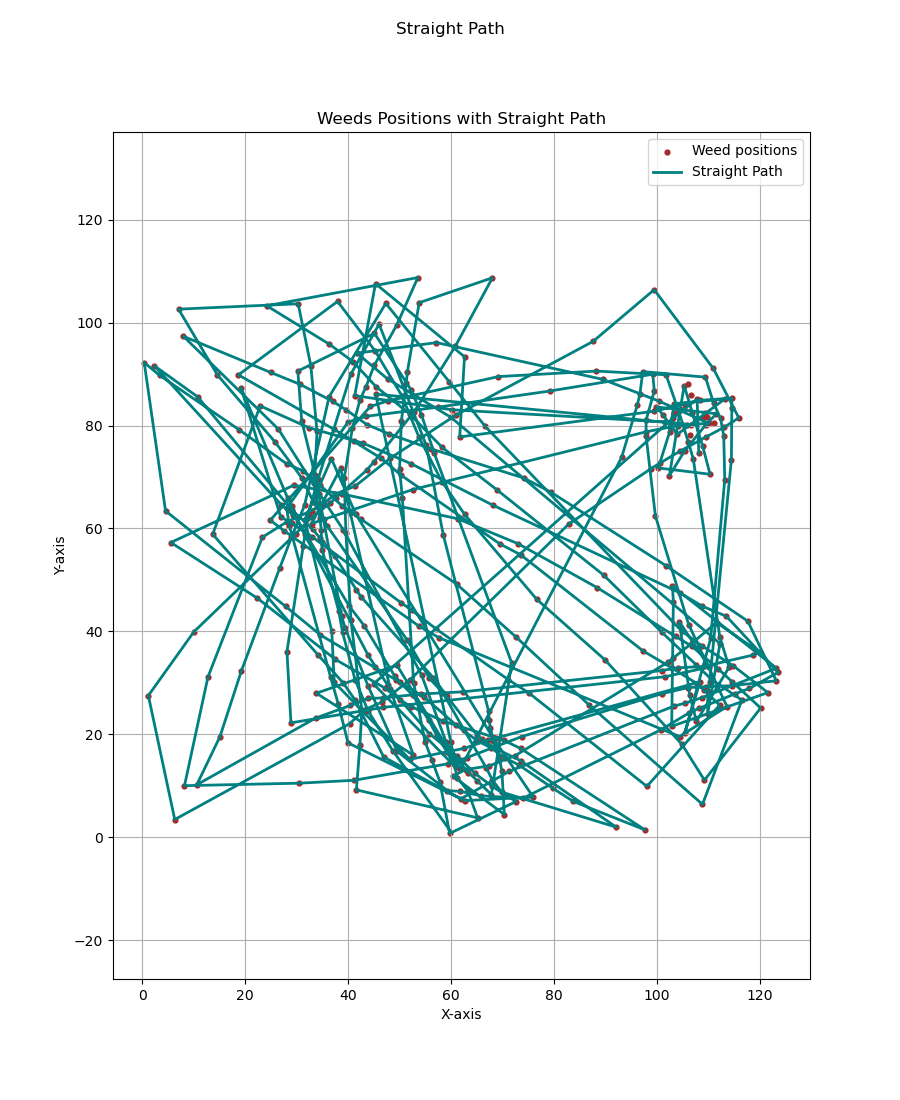
\includegraphics[height=36mm,width=0.24\textwidth]{Images/simulation_no_obs/straight_paths/13.png}
        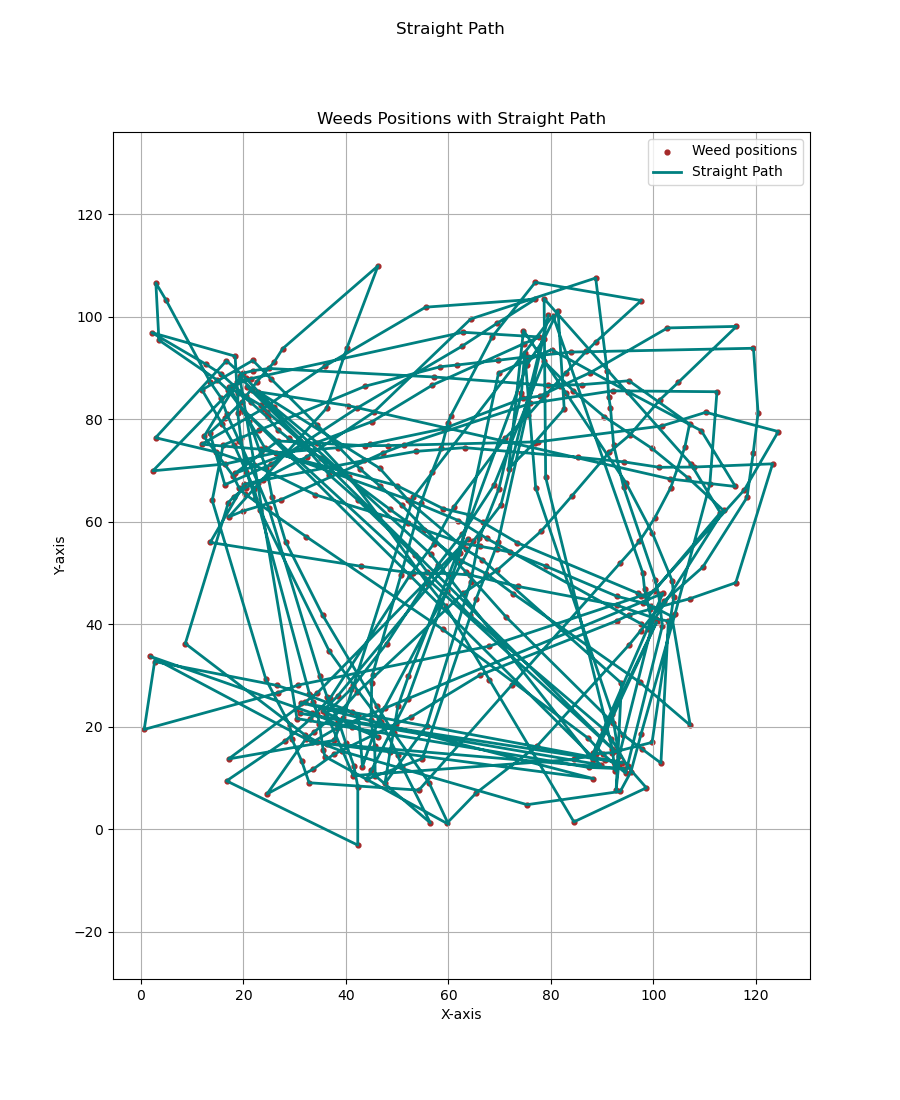
\includegraphics[height=36mm,width=0.24\textwidth]{Images/simulation_no_obs/straight_paths/14.png}\\[-4pt]

        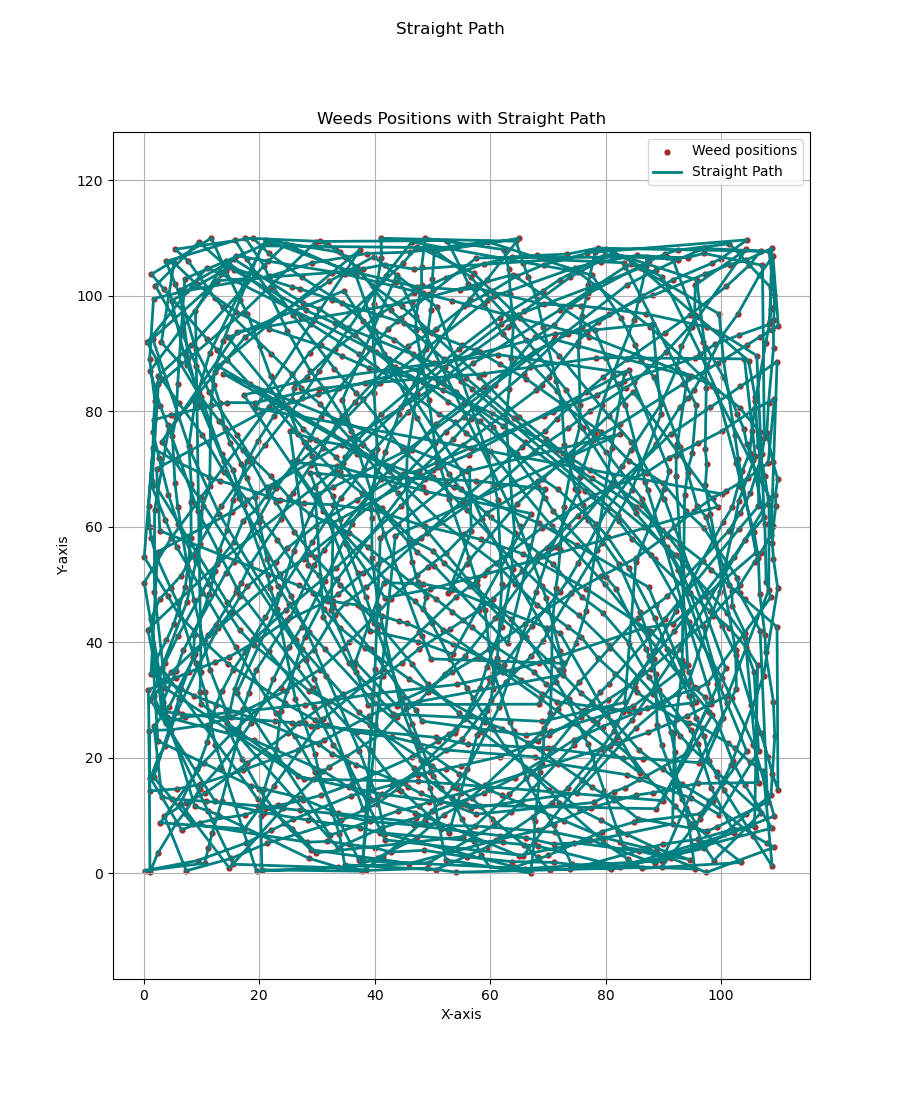
\includegraphics[height=36mm,width=0.24\textwidth]{Images/simulation_no_obs/straight_paths/21.png}
        & 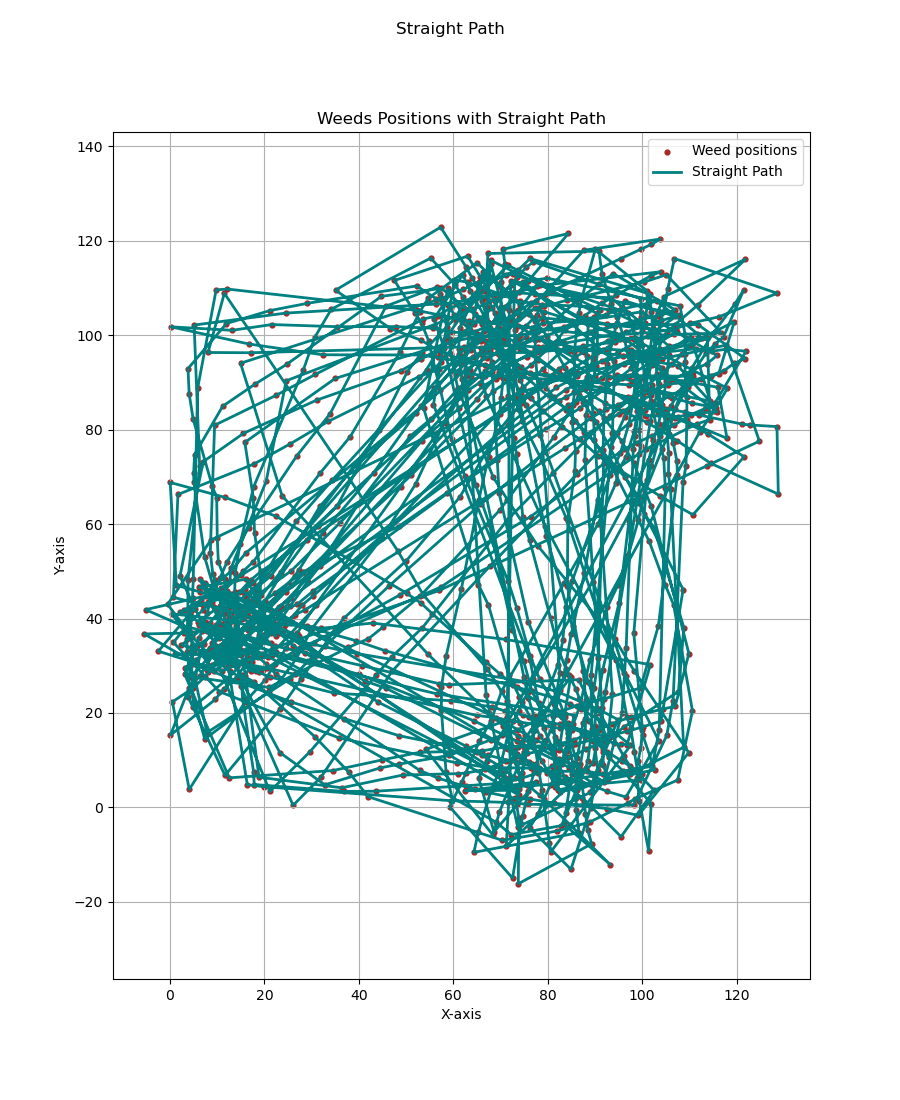
\includegraphics[height=36mm,width=0.24\textwidth]{Images/simulation_no_obs/straight_paths/22.png}
        & 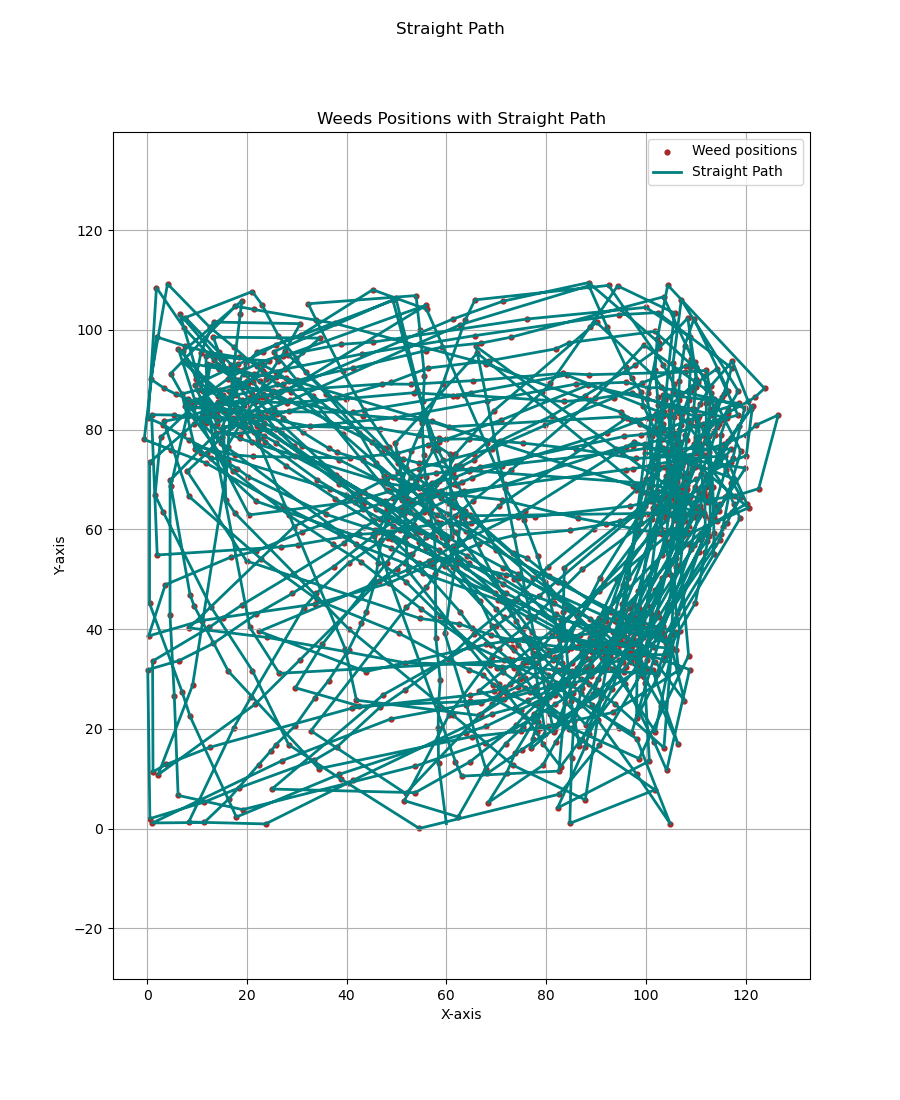
\includegraphics[height=36mm,width=0.24\textwidth]{Images/simulation_no_obs/straight_paths/23.png}
         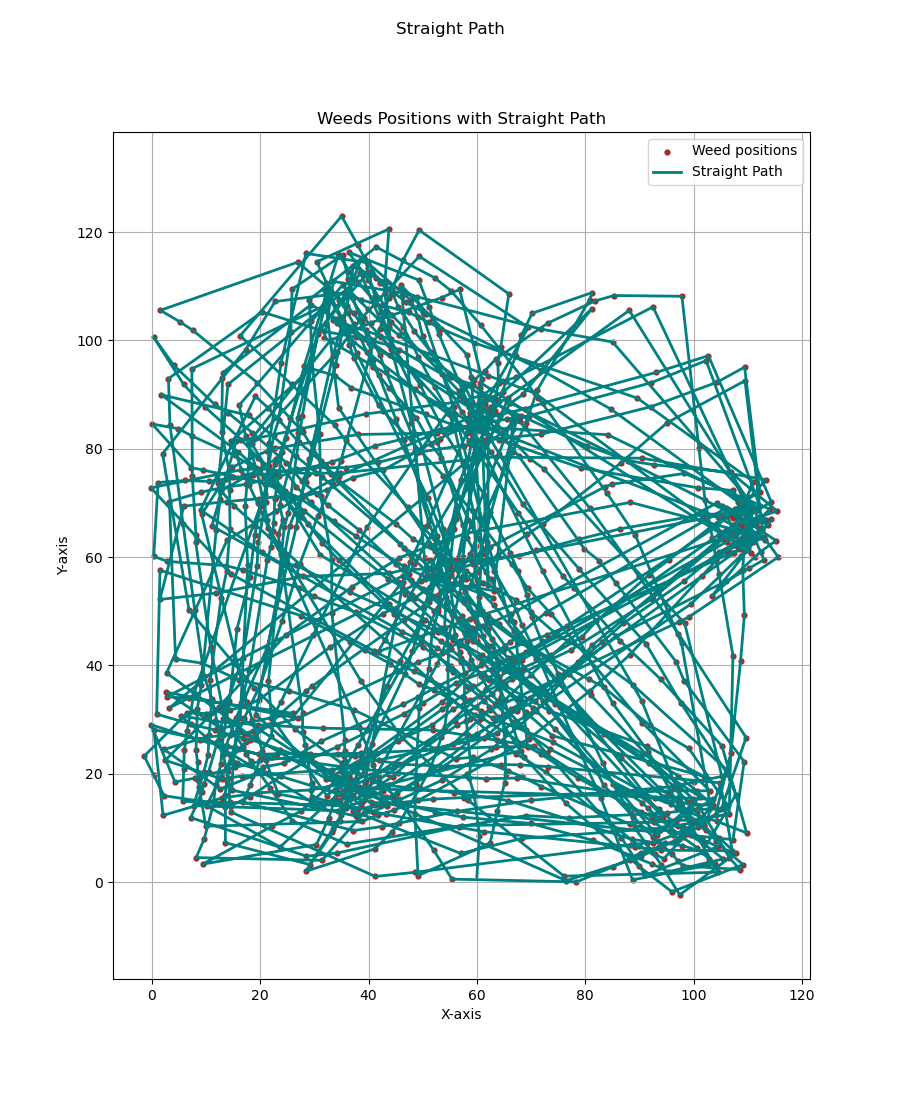
\includegraphics[height=36mm,width=0.24\textwidth]{Images/simulation_no_obs/straight_paths/24.png}\\[-4pt]

         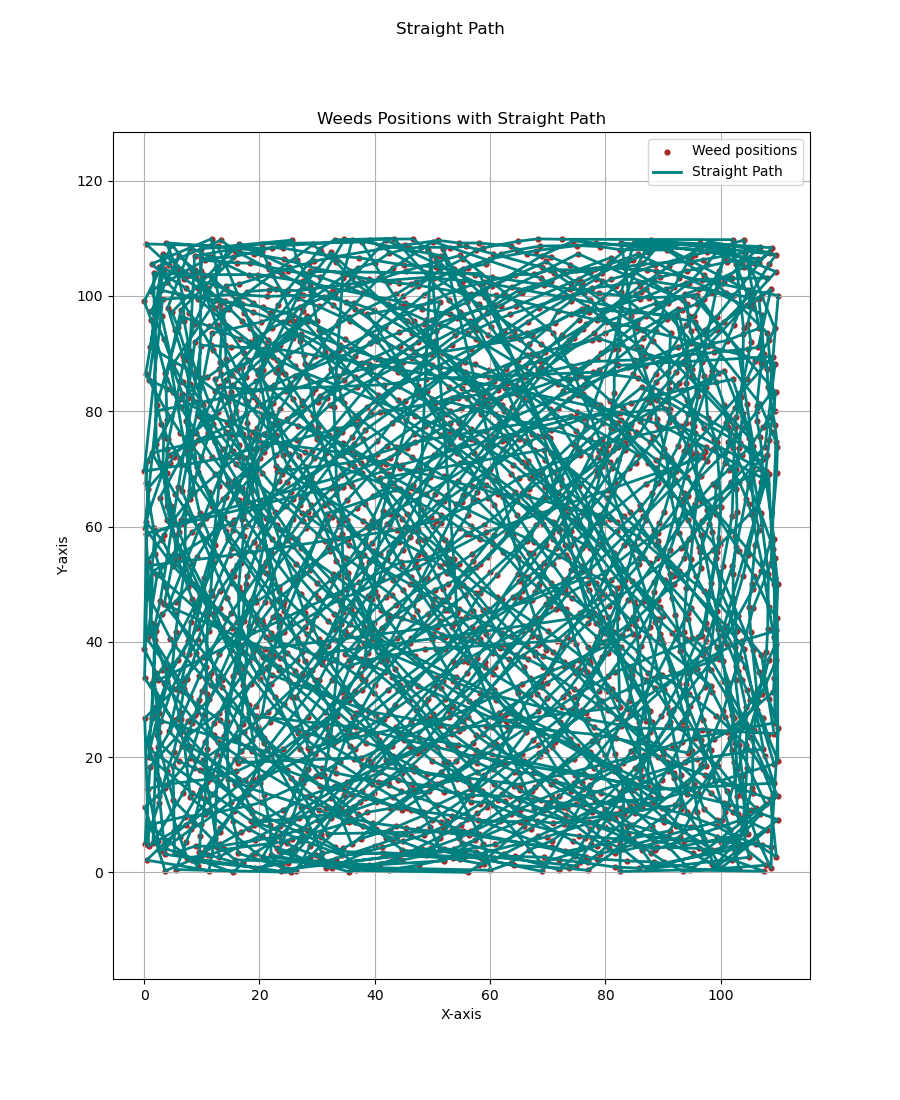
\includegraphics[height=36mm,width=0.24\textwidth]{Images/simulation_no_obs/straight_paths/31.png}
        & 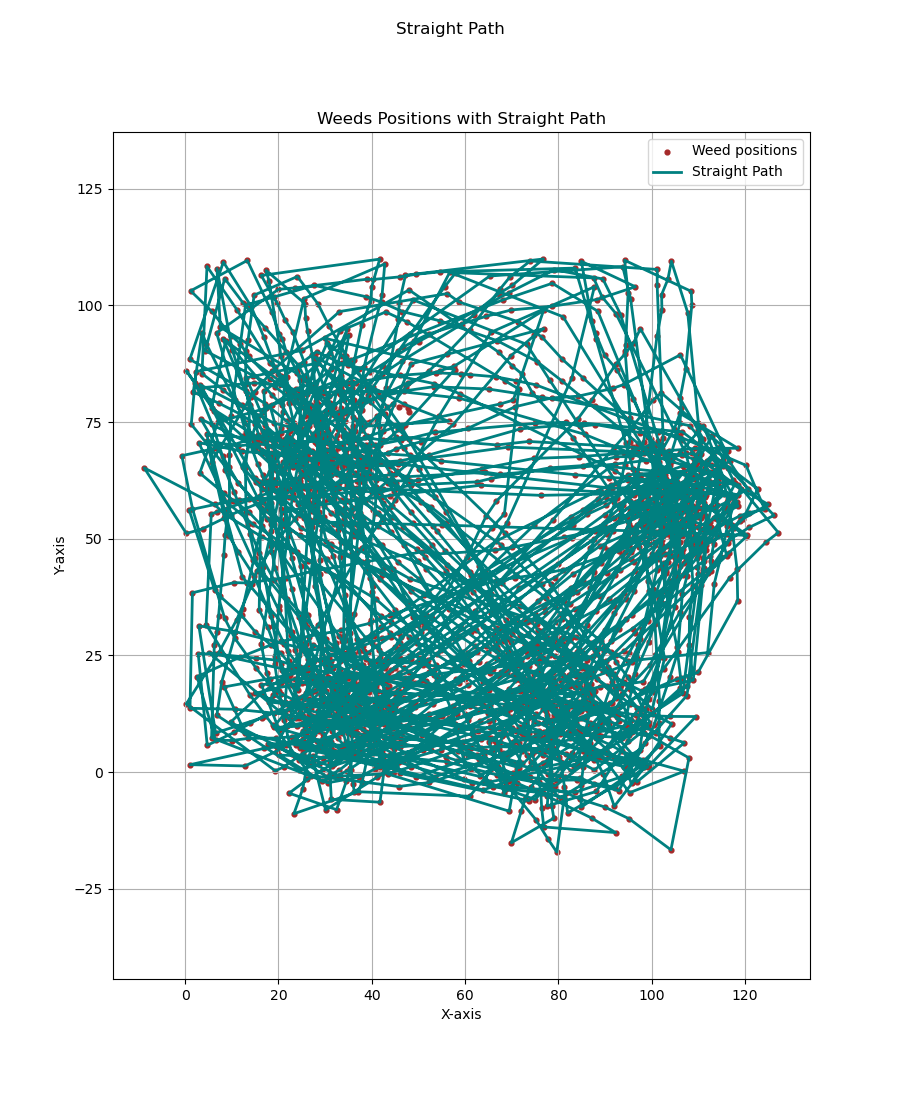
\includegraphics[height=36mm,width=0.24\textwidth]{Images/simulation_no_obs/straight_paths/32.png}
        & 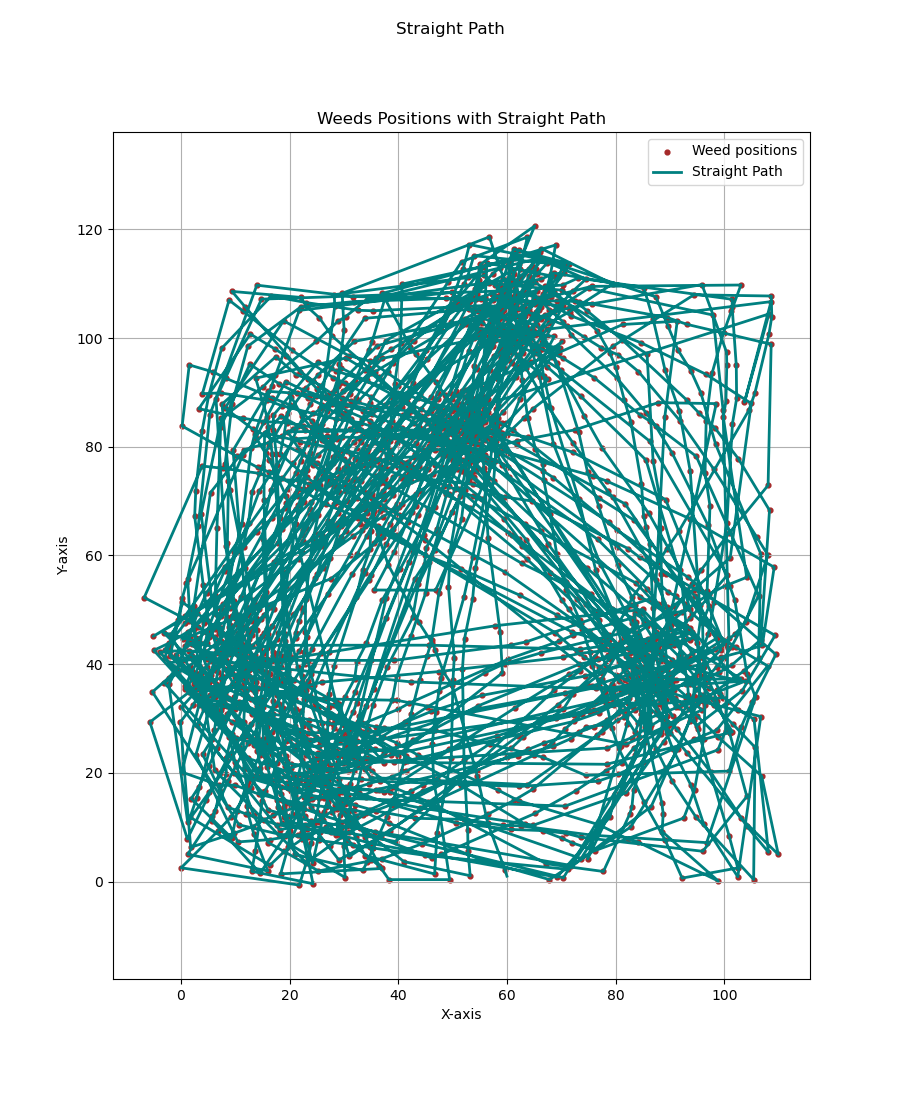
\includegraphics[height=36mm,width=0.24\textwidth]{Images/simulation_no_obs/straight_paths/33.png}
         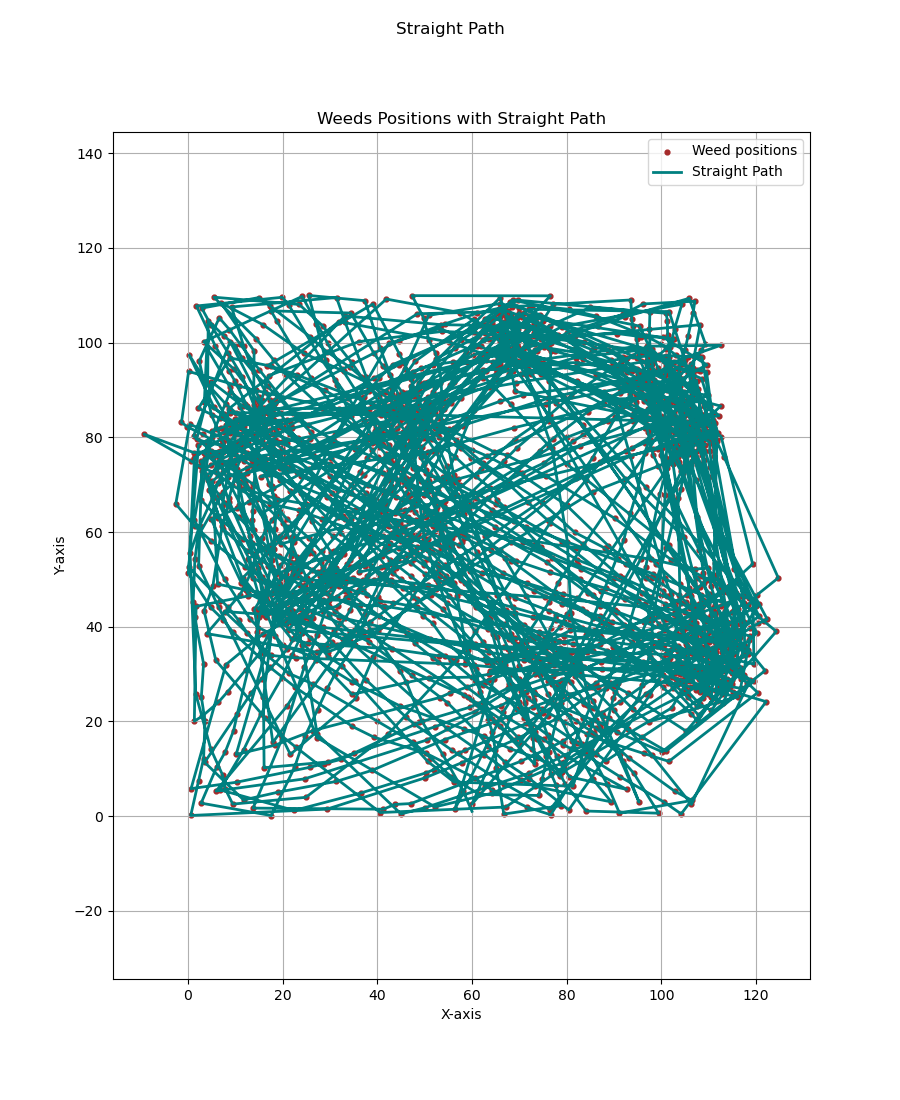
\includegraphics[height=36mm,width=0.24\textwidth]{Images/simulation_no_obs/straight_paths/34.png}\\[-4pt]


        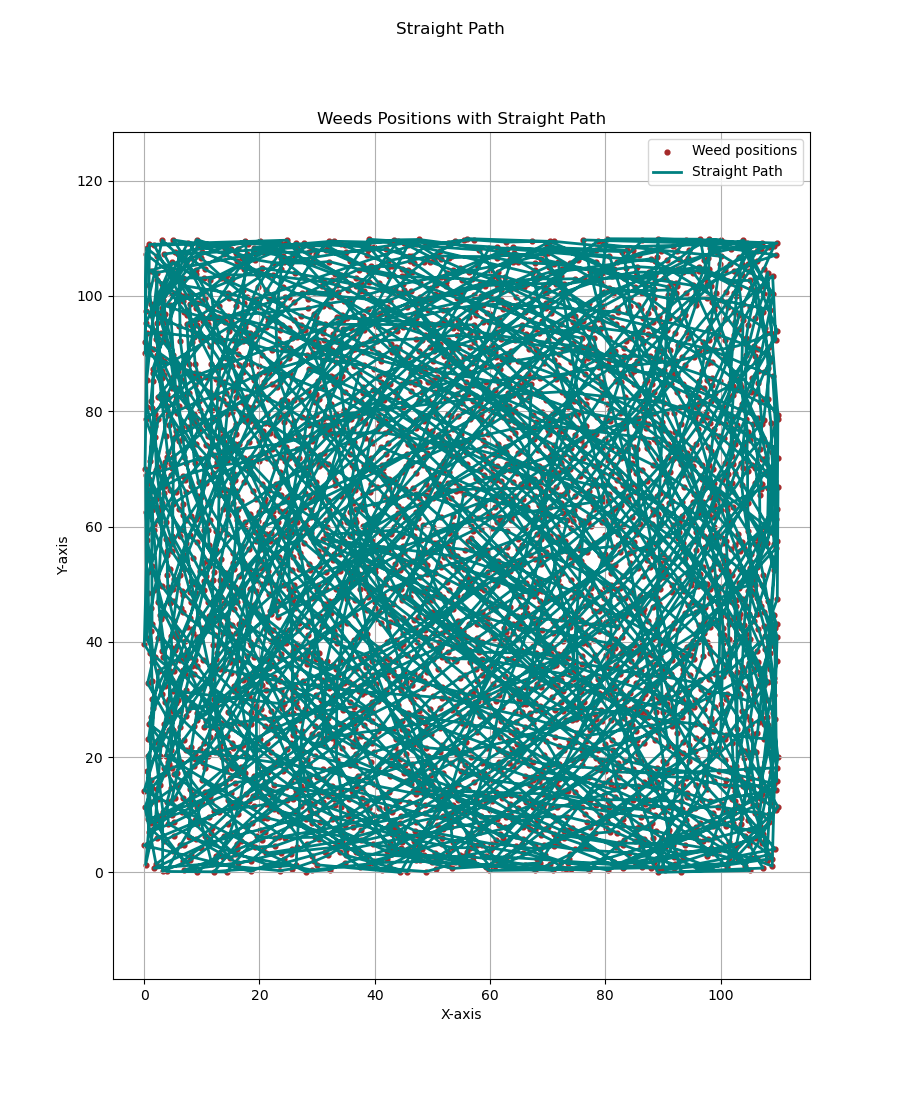
\includegraphics[height=36mm,width=0.24\textwidth]{Images/simulation_no_obs/straight_paths/41.png}
        & 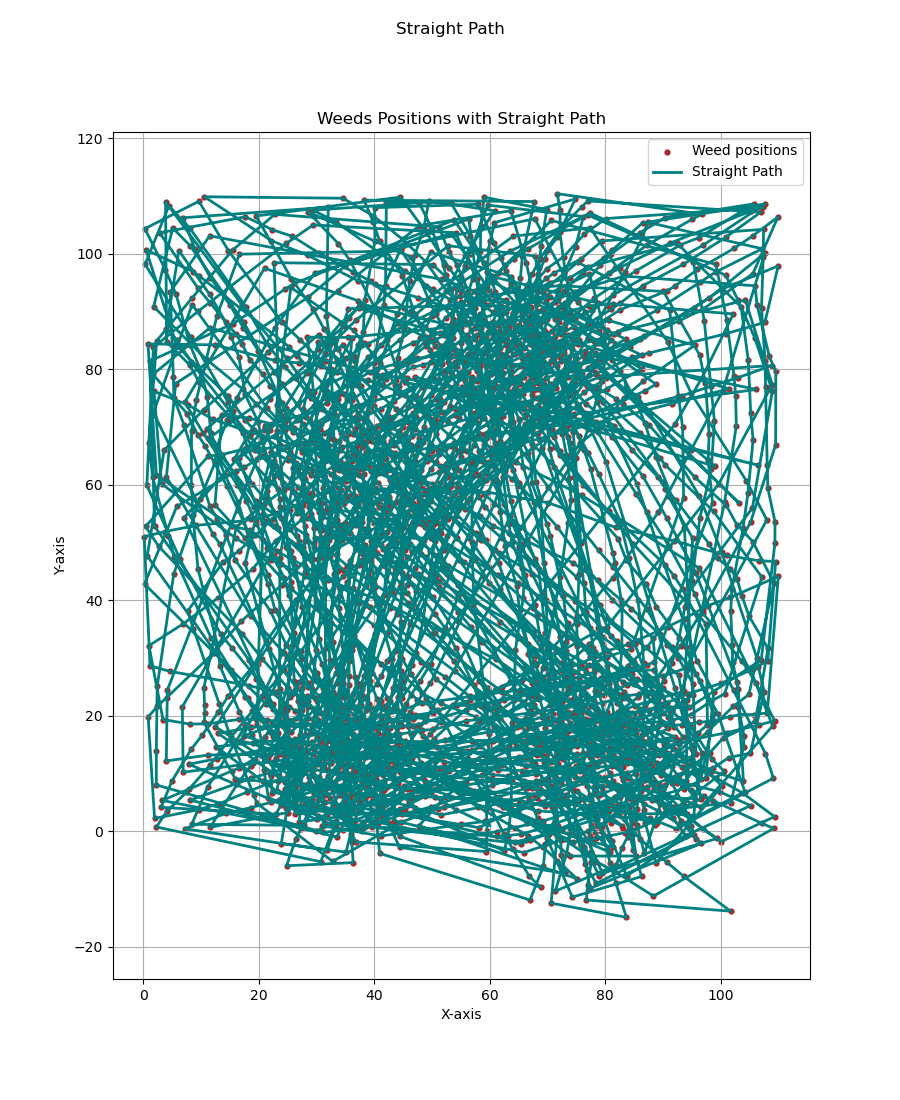
\includegraphics[height=36mm,width=0.24\textwidth]{Images/simulation_no_obs/straight_paths/42.png}
        & 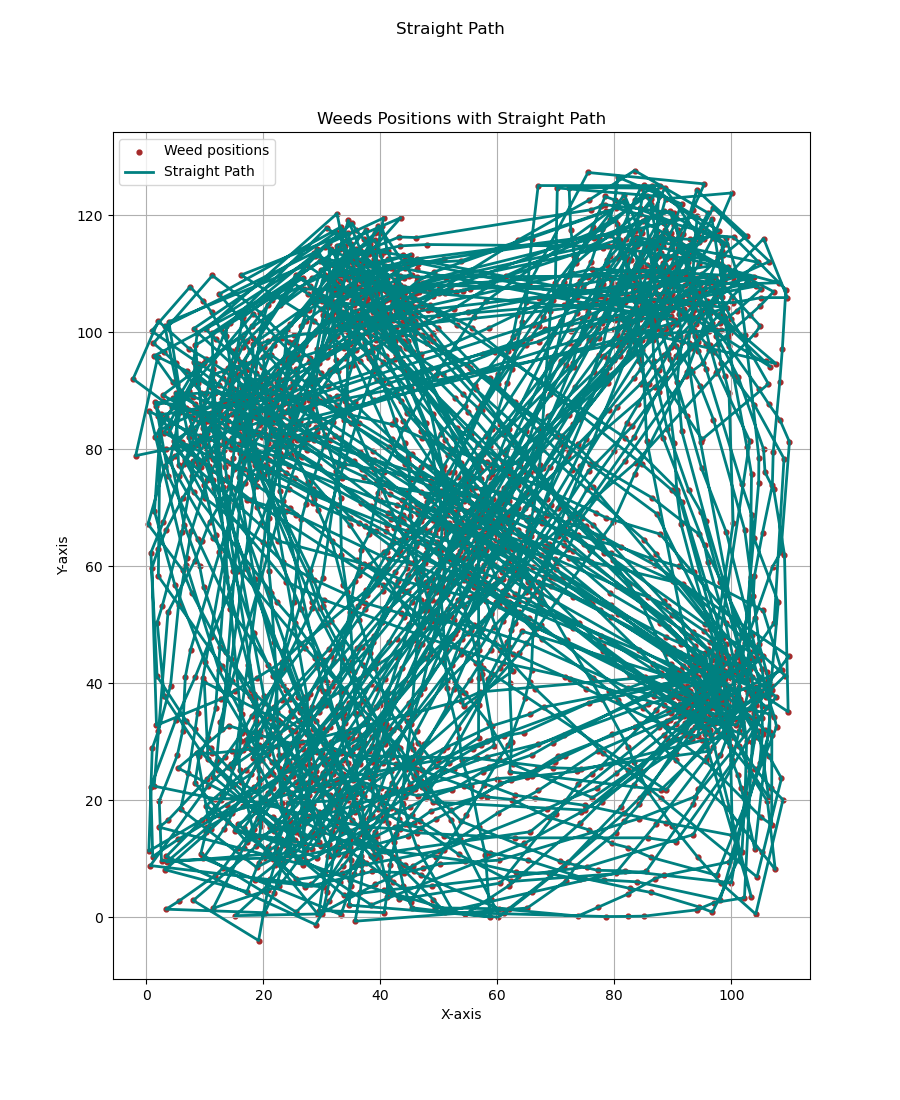
\includegraphics[height=36mm,width=0.24\textwidth]{Images/simulation_no_obs/straight_paths/43.png}
        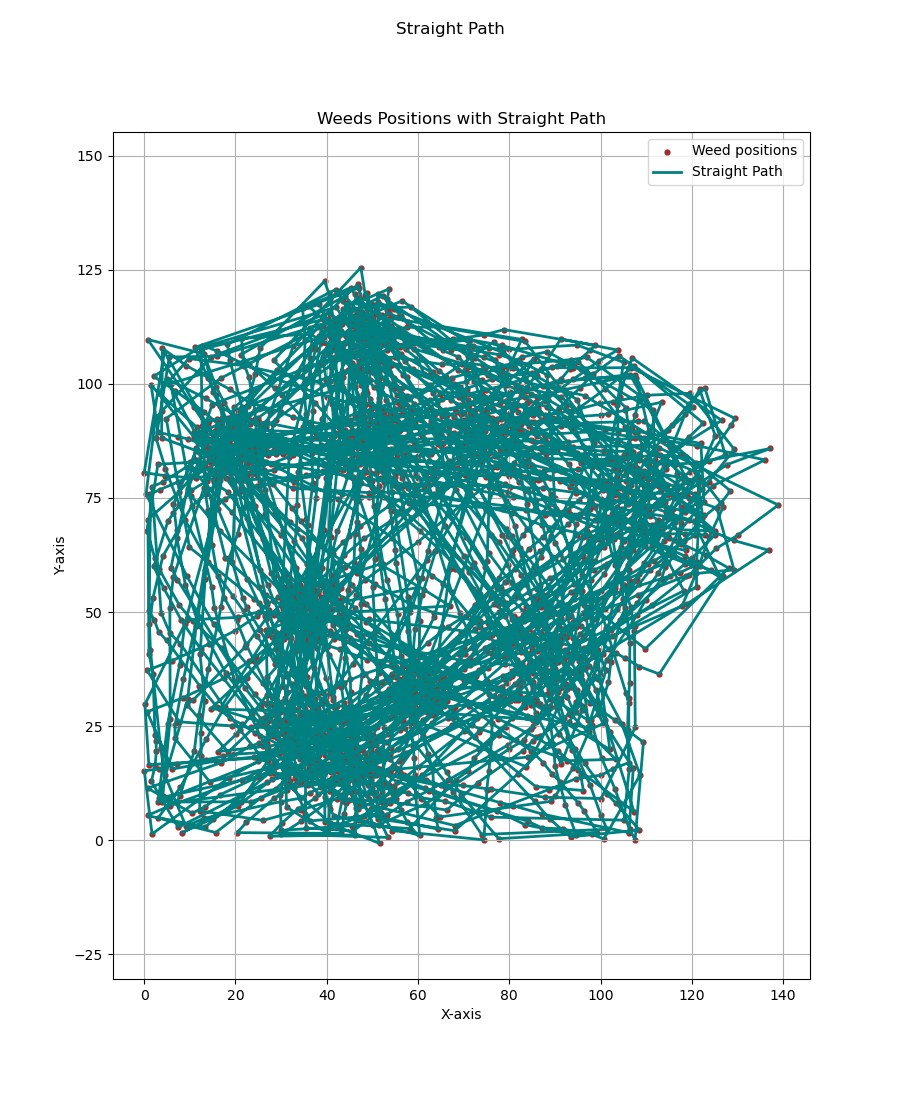
\includegraphics[height=36mm,width=0.24\textwidth]{Images/simulation_no_obs/straight_paths/44.png}\\[-4pt]

        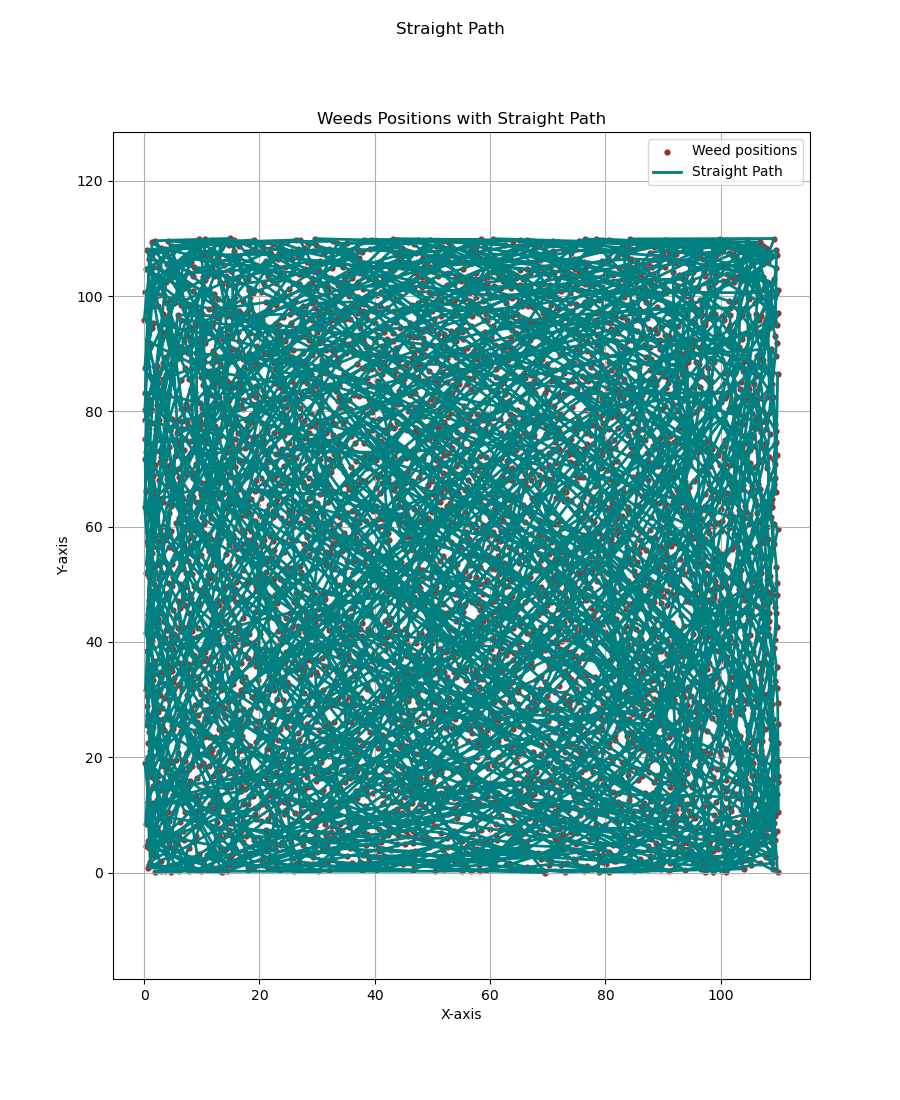
\includegraphics[height=36mm,width=0.24\textwidth]{Images/simulation_no_obs/straight_paths/51.png}
        & \includegraphics[height=36mm,width=0.24\textwidth]{Images/simulation_no_obs/straight_paths/52.png}
        & \includegraphics[height=36mm,width=0.24\textwidth]{Images/simulation_no_obs/straight_paths/53.png}
        \includegraphics[height=36mm,width=0.24\textwidth]{Images/simulation_no_obs/straight_paths/54.png}\\[-4pt]

    \end{tabular}
    \caption{Straight Path.\label{fig:straight_path}}
\end{figure}


\vspace{3mm}


Once the Dubins paths are generated from the straight paths, the resultant paths can be visualized in the (\autoref{fig:dubins_path}). These figures showcase the robot's traversal across different datasets, illustrating how the algorithm adapts to various point distributions.
% Dubin's path
\begin{figure}[p]
    \centering
    \begin{tabular}{ccc}
         \includegraphics[height=36mm,width=0.24\textwidth]{Images/simulation_no_obs/dubins_path/01.png}
        & \includegraphics[height=36mm,width=0.24\textwidth]{Images/simulation_no_obs/dubins_path/02.png}
        & \includegraphics[height=36mm,width=0.24\textwidth]{Images/simulation_no_obs/dubins_path/03.png}
         \includegraphics[height=36mm,width=0.24\textwidth]{Images/simulation_no_obs/dubins_path/04.png}\\[-4pt]

        \includegraphics[height=36mm,width=0.24\textwidth]{Images/simulation_no_obs/dubins_path/11.png}
        & \includegraphics[height=36mm,width=0.24\textwidth]{Images/simulation_no_obs/dubins_path/12.png}
        & \includegraphics[height=36mm,width=0.24\textwidth]{Images/simulation_no_obs/dubins_path/13.png}
        \includegraphics[height=36mm,width=0.24\textwidth]{Images/simulation_no_obs/dubins_path/14.png}\\[-4pt]

        \includegraphics[height=36mm,width=0.24\textwidth]{Images/simulation_no_obs/dubins_path/21.png}
        & \includegraphics[height=36mm,width=0.24\textwidth]{Images/simulation_no_obs/dubins_path/22.png}
        & \includegraphics[height=36mm,width=0.24\textwidth]{Images/simulation_no_obs/dubins_path/23.png}
         \includegraphics[height=36mm,width=0.24\textwidth]{Images/simulation_no_obs/dubins_path/24.png}\\[-4pt]

         \includegraphics[height=36mm,width=0.24\textwidth]{Images/simulation_no_obs/dubins_path/31.png}
        & \includegraphics[height=36mm,width=0.24\textwidth]{Images/simulation_no_obs/dubins_path/32.png}
        & \includegraphics[height=36mm,width=0.24\textwidth]{Images/simulation_no_obs/dubins_path/33.png}
         \includegraphics[height=36mm,width=0.24\textwidth]{Images/simulation_no_obs/dubins_path/34.png}\\[-4pt]


        \includegraphics[height=36mm,width=0.24\textwidth]{Images/simulation_no_obs/dubins_path/41.png}
        & \includegraphics[height=36mm,width=0.24\textwidth]{Images/simulation_no_obs/dubins_path/42.png}
        & \includegraphics[height=36mm,width=0.24\textwidth]{Images/simulation_no_obs/dubins_path/43.png}
        \includegraphics[height=36mm,width=0.24\textwidth]{Images/simulation_no_obs/dubins_path/44.png}\\[-4pt]

        \includegraphics[height=36mm,width=0.24\textwidth]{Images/simulation_no_obs/dubins_path/51.png}
        & \includegraphics[height=36mm,width=0.24\textwidth]{Images/simulation_no_obs/dubins_path/52.png}
        & \includegraphics[height=36mm,width=0.24\textwidth]{Images/simulation_no_obs/dubins_path/53.png}
        \includegraphics[height=36mm,width=0.24\textwidth]{Images/simulation_no_obs/dubins_path/54.png}\\[-4pt]

    \end{tabular}
    \caption{Dubin's Path.\label{fig:dubins_path}}
\end{figure}



\vspace{3mm}

The performance metrics for all datasets are summarized in the (\autoref{tab:performance_metrics}). These metrics provide insights into the algorithm's computational efficiency, operational effectiveness, and overall robustness.

% Metrics for CPP.
\begin{table}[]
    \centering
    \caption{Results for the performance metrics.}
    \label{tab:performance_metrics}
    \small
    \begin{tabular}{cllllll}
    \hline
    \rowcolor[HTML]{67D5DA} 
    \multicolumn{1}{l}{\cellcolor[HTML]{67D5DA}\textit{\textbf{\begin{tabular}[c]{@{}l@{}}No. of\\  points\end{tabular}}}} & \textit{\textbf{Cases}} & \textit{\textbf{\begin{tabular}[c]{@{}l@{}}Computation \\ Time in secs.\end{tabular}}} & \textit{\textbf{\begin{tabular}[c]{@{}l@{}}Field Operation\\  Time in sec.\end{tabular}}} & \textit{\textbf{\begin{tabular}[c]{@{}l@{}}Route length\\  in meters\end{tabular}}} & \textit{\textbf{\begin{tabular}[c]{@{}l@{}}No. of \\ Turns.\end{tabular}}} & \textit{\textbf{\begin{tabular}[c]{@{}l@{}}Energy \\ Consumption \\ in KWh.\end{tabular}}} \\ \hline
    \rowcolor[HTML]{FFFFC7} 
    \cellcolor[HTML]{FFFFC7}                                                                                               & case 1                  & 0.858553886                                                                            & 6282.400938                                                                               & 4652.945                                                                            & 48                                                                         & 5783.34459                                                                                 \\ \cline{2-7} 
    \rowcolor[HTML]{FFFFC7} 
    \cellcolor[HTML]{FFFFC7}                                                                                               & case 2                  & 0.775789261                                                                            & 5125.168209                                                                               & 3769.005                                                                            & 41                                                                         & 4734.555207                                                                                \\ \cline{2-7} 
    \rowcolor[HTML]{FFFFC7} 
    \cellcolor[HTML]{FFFFC7}                                                                                               & case 3                  & 0.788151503                                                                            & 5413.822753                                                                               & 3985.978                                                                            & 44                                                                         & 5022.177564                                                                                \\ \cline{2-7} 
    \rowcolor[HTML]{FFFFC7} 
    \multirow{-4}{*}{\cellcolor[HTML]{FFFFC7}250}                                                                          & case 4                  & 0.825942278                                                                            & 6216.01818                                                                                & 4620.695                                                                            & 44                                                                         & 5656.894864                                                                                \\ \hline
    \rowcolor[HTML]{FFFFC7} 
    \cellcolor[HTML]{FFFFC7}                                                                                               & case 1                  & 1.842700005                                                                            & 9520.140257                                                                               & 7027.363                                                                            & 75                                                                         & 8793.612844                                                                                \\ \cline{2-7} 
    \rowcolor[HTML]{FFFFC7} 
    \cellcolor[HTML]{FFFFC7}                                                                                               & case 2                  & 1.696401358                                                                            & 9151.211911                                                                               & 6788.619                                                                            & 67                                                                         & 8366.468569                                                                                \\ \cline{2-7} 
    \rowcolor[HTML]{FFFFC7} 
    \cellcolor[HTML]{FFFFC7}                                                                                               & case 3                  & 1.940592766                                                                            & 8589.717644                                                                               & 6336.544                                                                            & 67                                                                         & 7914.394434                                                                                \\ \cline{2-7} 
    \rowcolor[HTML]{FFFFC7} 
    \multirow{-4}{*}{\cellcolor[HTML]{FFFFC7}500}                                                                          & case 4                  & 1.609200478                                                                            & 9761.624722                                                                               & 7250.2                                                                              & 70                                                                         & 8898.700417                                                                                \\ \hline
    \rowcolor[HTML]{FFFFC7} 
    \cellcolor[HTML]{FFFFC7}                                                                                               & case 1                  & 9.04812026                                                                             & 21751.64778                                                                               & 16189.858                                                                           & 154                                                                        & 19816.55759                                                                                \\ \cline{2-7} 
    \rowcolor[HTML]{FFFFC7} 
    \cellcolor[HTML]{FFFFC7}                                                                                               & case 2                  & 8.591621161                                                                            & 22226.37676                                                                               & 16650.701                                                                           & 144                                                                        & 20041.90077                                                                                \\ \cline{2-7} 
    \rowcolor[HTML]{FFFFC7} 
    \cellcolor[HTML]{FFFFC7}                                                                                               & case 3                  & 7.65038085                                                                             & 18446.73883                                                                               & 13728.721                                                                           & 131                                                                        & 16813.77138                                                                                \\ \cline{2-7} 
    \rowcolor[HTML]{FFFFC7} 
    \multirow{-4}{*}{\cellcolor[HTML]{FFFFC7}2000}                                                                         & case 4                  & 8.155776024                                                                            & 20839.67217                                                                               & 15547.469                                                                           & 139                                                                        & 18820.91894                                                                                \\ \hline
    \rowcolor[HTML]{FFFFC7} 
    \cellcolor[HTML]{FFFFC7}                                                                                               & case 1                  & 24.18394971                                                                            & 32301.69933                                                                               & 24191.259                                                                           & 210                                                                        & 29136.75914                                                                                \\ \cline{2-7} 
    \rowcolor[HTML]{FFFFC7} 
    \cellcolor[HTML]{FFFFC7}                                                                                               & case 2                  & 20.85941482                                                                            & 29871.08874                                                                               & 22356.011                                                                           & 198                                                                        & 27018.91147                                                                                \\ \cline{2-7} 
    \rowcolor[HTML]{FFFFC7} 
    \cellcolor[HTML]{FFFFC7}                                                                                               & case 3                  & 18.23963118                                                                            & 27659.4681                                                                                & 20620.054                                                                           & 192                                                                        & 25141.65448                                                                                \\ \cline{2-7} 
    \rowcolor[HTML]{FFFFC7} 
    \multirow{-4}{*}{\cellcolor[HTML]{FFFFC7}4000}                                                                         & case 4                  & 19.22349644                                                                            & 29701.58872                                                                               & 22222.31                                                                            & 200                                                                        & 26932.31049                                                                                \\ \hline
    \rowcolor[HTML]{FFFFC7} 
    \cellcolor[HTML]{FFFFC7}                                                                                               & case 1                  & 45.23673987                                                                            & 39851.80224                                                                               & 29777.382                                                                           & 262                                                                        & 35947.48179                                                                                \\ \cline{2-7} 
    \rowcolor[HTML]{FFFFC7} 
    \cellcolor[HTML]{FFFFC7}                                                                                               & case 2                  & 33.23154497                                                                            & 34821.16749                                                                               & 26039.854                                                                           & 236                                                                        & 31597.65399                                                                                \\ \cline{2-7} 
    \rowcolor[HTML]{FFFFC7} 
    \cellcolor[HTML]{FFFFC7}                                                                                               & case 3                  & 30.80121374                                                                            & 35035.83592                                                                               & 26223.169                                                                           & 230                                                                        & 31639.66906                                                                                \\ \cline{2-7} 
    \rowcolor[HTML]{FFFFC7} 
    \multirow{-4}{*}{\cellcolor[HTML]{FFFFC7}6000}                                                                         & case 4                  & 32.34737062                                                                            & 35496.36509                                                                               & 26570.832                                                                           & 226                                                                        & 31893.13207                                                                                \\ \hline
    \rowcolor[HTML]{FFFFC7} 
    \cellcolor[HTML]{FFFFC7}                                                                                               & case 1                  & 122.6808474                                                                            & 50681.89334                                                                               & 38128.675                                                                           & 308                                                                        & 45382.07468                                                                                \\ \cline{2-7} 
    \rowcolor[HTML]{FFFFC7} 
    \cellcolor[HTML]{FFFFC7}                                                                                               & case 2                  & 74.37674475                                                                            & 45367.87779                                                                               & 34118.252                                                                           & 277                                                                        & 40641.60223                                                                                \\ \cline{2-7} 
    \rowcolor[HTML]{FFFFC7} 
    \cellcolor[HTML]{FFFFC7}                                                                                               & case 3                  & 65.54510021                                                                            & 42291.24514                                                                               & 31650.696                                                                           & 278                                                                        & 38197.59611                                                                                \\ \cline{2-7} 
    \rowcolor[HTML]{FFFFC7} 
    \multirow{-4}{*}{\cellcolor[HTML]{FFFFC7}10000}                                                                        & case 4                  & 62.76576424                                                                            & 42801.16425                                                                               & 32154.031                                                                           & 274                                                                        & 38606.73138                                                                                \\ \hline
    \end{tabular}
    \end{table}



\vspace{3mm} 


The coverage rate plot over the field time offers a visual representation of the algorithm's performance across the whole datasets. This plot demonstrates how effectively the algorithm achieves coverage over time, allowing for a comparative analysis of its efficiency under varying point distributions and densities. This plot can be visualized in (\autoref{fig:coverage_plots}).   

% Coverage rate plot
\begin{figure}[p]
    \centering
    \begin{tabular}{ccc}
         \includegraphics[height=36mm,width=0.24\textwidth]{Images/simulation_no_obs/coverage_plots/01.png}
        & \includegraphics[height=36mm,width=0.24\textwidth]{Images/simulation_no_obs/coverage_plots/02.png}
        & \includegraphics[height=36mm,width=0.24\textwidth]{Images/simulation_no_obs/coverage_plots/03.png}
         \includegraphics[height=36mm,width=0.24\textwidth]{Images/simulation_no_obs/coverage_plots/04.png}\\[-4pt]

        \includegraphics[height=36mm,width=0.24\textwidth]{Images/simulation_no_obs/coverage_plots/11.png}
        & \includegraphics[height=36mm,width=0.24\textwidth]{Images/simulation_no_obs/coverage_plots/12.png}
        & \includegraphics[height=36mm,width=0.24\textwidth]{Images/simulation_no_obs/coverage_plots/13.png}
        \includegraphics[height=36mm,width=0.24\textwidth]{Images/simulation_no_obs/coverage_plots/14.png}\\[-4pt]

        \includegraphics[height=36mm,width=0.24\textwidth]{Images/simulation_no_obs/coverage_plots/21.png}
        & \includegraphics[height=36mm,width=0.24\textwidth]{Images/simulation_no_obs/coverage_plots/22.png}
        & \includegraphics[height=36mm,width=0.24\textwidth]{Images/simulation_no_obs/coverage_plots/23.png}
         \includegraphics[height=36mm,width=0.24\textwidth]{Images/simulation_no_obs/coverage_plots/24.png}\\[-4pt]

         \includegraphics[height=36mm,width=0.24\textwidth]{Images/simulation_no_obs/coverage_plots/31.png}
        & \includegraphics[height=36mm,width=0.24\textwidth]{Images/simulation_no_obs/coverage_plots/32.png}
        & \includegraphics[height=36mm,width=0.24\textwidth]{Images/simulation_no_obs/coverage_plots/33.png}
         \includegraphics[height=36mm,width=0.24\textwidth]{Images/simulation_no_obs/coverage_plots/34.png}\\[-4pt]


        \includegraphics[height=36mm,width=0.24\textwidth]{Images/simulation_no_obs/coverage_plots/41.png}
        & \includegraphics[height=36mm,width=0.24\textwidth]{Images/simulation_no_obs/coverage_plots/42.png}
        & \includegraphics[height=36mm,width=0.24\textwidth]{Images/simulation_no_obs/coverage_plots/43.png}
        \includegraphics[height=36mm,width=0.24\textwidth]{Images/simulation_no_obs/coverage_plots/44.png}\\[-4pt]

        \includegraphics[height=36mm,width=0.24\textwidth]{Images/simulation_no_obs/coverage_plots/51.png}
        & \includegraphics[height=36mm,width=0.24\textwidth]{Images/simulation_no_obs/coverage_plots/52.png}
        & \includegraphics[height=36mm,width=0.24\textwidth]{Images/simulation_no_obs/coverage_plots/53.png}
        \includegraphics[height=36mm,width=0.24\textwidth]{Images/simulation_no_obs/coverage_plots/54.png}\\[-4pt]

    \end{tabular}
    \caption{Coverage plots.\label{fig:coverage_plots}}
    \end{figure}


The performance metrics plots provide a visual representation for better understanding of the algorithm's performance across different datasets. Therefore, separate plots for each performance metric are generated to analyze the algorithm's performance under varying scenarios. These plots can be visualized in the (\autoref{fig:Computation_time}), (\autoref{fig:Energy_expenditure}), (\autoref{fig:Route_length}), and (\autoref{fig:Field_operation_time}).


\begin{figure}[H]
    \centering
    \includegraphics[width=\textwidth]{Images/plots/no_obs/Computation_time.png}
    \caption{Computation Time.}
    \label{fig:Computation_time}
\end{figure}

\begin{figure}[H]
    \centering
    \includegraphics[width=\textwidth]{Images/plots/no_obs/Energy.png}
    \caption{Energy Expenditure.}
    \label{fig:Energy_expenditure}
\end{figure}

\begin{figure}[H]
    \centering
    \includegraphics[width=\textwidth]{Images/plots/no_obs/Route_length.png}
    \caption{Route Length.}
    \label{fig:Route_length}
\end{figure}

\begin{figure}[H]
    \centering
    \includegraphics[width=\textwidth]{Images/plots/no_obs/Field_time.png}
    \caption{Field Operation Time.}
    \label{fig:Field_operation_time}
\end{figure}


The proposed algorithm operates by initially generating straight paths and subsequently applying Dubins paths to ensure feasibility given the robot's constraints. The straight paths, as visualized in the initial results, are approximately linear, aiming to cover the maximum number of points while maintaining minimal path length. This demonstrates the algorithm's ability to generate efficient coverage paths.

\vspace{3mm} 

The Dubins path results further validate the algorithm's capability to model the robot's constraints effectively. An inability to model these constraints accurately would result in numerous infeasible circular paths. The primary objective of employing this behavioral approach is to sustain a high coverage rate from start to finish across various data distributions. The results indicate that the algorithm successfully maintains a high coverage rate irrespective of the distribution type. It is noteworthy that the coverage rate is initially very high and gradually decreases, attributed to the diminishing number of points left to cover after a significant percentage of coverage. Nonetheless, the coverage rate remains high, indicating efficient coverage by the algorithm. The percentage coverage also suggests that the point at which the algorithm changes behavior is near-optimal; otherwise, a gradual increase in coverage rate would be observed if the change occurred at a different percentage.

\vspace{3mm} 

The computation time plot across all datasets indicates an expected increase in computation time with the number of points. However, the rise in computation time is notable. For instance, even in the largest case of 10,000 points with random distribution, the computation time is 122.68 seconds, which is remarkably low as compared to current state-of-the-art approaches following the non-holonoomic constraints. This efficiency is further highlighted by the average computation time of 60 seconds for other scenarios, demonstrating the algorithm's computational efficiency. This is particularly significant as no real agricultural field would have a purely random distribution, making the algorithm's performance even more impressive in practical scenarios.

\vspace{3mm} 

Similarly, the route length increases with the number of points as the robot needs to traverse more straight lines to cover all points. It is noteworthy that the maximum route length for each dataset occurs with random distribution and decreases significantly with fewer clusters, increasing again as the number of clusters rises.

\vspace{3mm} 

Field operation time and energy consumption are derived from the route length, factoring in the robot's maximum allowable velocity on straight and curved paths. The robot can move at twice the speed on straight paths compared to curved paths without damaging crops. The parameters used for the current robot, as outlined in the table, provide a close approximation of real values, although the exact curved distance is challenging to estimate with this pipeline. Energy consumption is approximated to be four times higher on curved paths than on straight paths. The plots above reflect these estimations. 



\newpage 


\chapter{Simulation Test and Analysis with obstacles} 


This section presents a comprehensive examination of the proposed complete coverage path planning algorithm, tailored to handle static polygonal obstacles in agricultural field applications. The section is divided into two key parts: Simulation Setup and Results \& Analysis.

\section{Simulation Setup}

This subsection provides a detailed description of the simulation setup, focusing on the experimental framework within which the tests are conducted.

\vspace{3mm}  


The simulation environment is meticulously crafted to replicate real-world agricultural fields, incorporating static polygonal obstacles to simulate common structures such as trees, rocks, or buildings that serve as keep-out zones. This realistic setup ensures that the algorithm's performance is rigorously evaluated under practical conditions.

\vspace{3mm}  

This simulation environment is setup utilizing a realistic field data obtained from the field manually and inclusion of the obstacles within the field. While the point distribution remains unchanged, the obstacles' shapes, sizes, and numbers vary across different scenarios. Strategic placement of obstacles tests the algorithm's adaptability and robustness. Five distinct datasets are used to assess the algorithm's performance under varying obstacle configurations, increasing in complexity with each set.



\vspace{3mm}  

Dataset Description

To thoroughly evaluate the algorithm, five distinct datasets are employed within a flat 120m x 120m field, each containing different numbers and configurations of obstacles:

\begin{itemize}
    \item Set1: Contains one rectangular obstacle of size 10m x 10m.
    \item Set2: Contains two rectangular obstacles of sizes 10m x 10m and 4m x 4m.
    \item Set3: Contains three convex polygonal obstacles of distinct sizes and shapes.
    \item Set4: Contains six convex polygonal obstacles of different sizes and shapes.
    \item Set5: Contains six polygonal obstacles of varying sizes and shapes, including concave and extremely long obstacles.
\end{itemize}
This hierarchical arrangement of datasets, with increasing complexity, ensures comprehensive testing of the algorithm's robustness and adaptability to real-world agricultural environments, where obstacles can vary significantly.

\vspace{3mm}  

Performance Metrics
The algorithm's performance is evaluated using several critical metrics across all datasets:

\begin{itemize}
    \item Computational Time: The time required for the algorithm to compute the coverage path.
    \item Field Operation Time: The actual time taken for the robot to complete the coverage task.
    \item Total Path Length: The total distance traveled by the robot.
    \item Number of Turns: The total number of turns the robot makes during its operation.
    \item Energy Consumption: The energy used by the robot to complete the coverage task.
    \item Coverage Efficiency: The percentage of points covered by the robot within the operational time.
\end{itemize}
These metrics provide a comprehensive assessment of the algorithm's efficiency, effectiveness, and overall performance under different test scenarios.


\vspace{3mm}  

\textbf{Visual Representation of the Dataset}

The (\autoref{fig:obstacles_dataset}) illustrates the five different datasets used in the simulation experiments, showcasing the shapes, sizes, numbers, and locations of obstacles within the field. This visual representation aids in understanding the varying complexities introduced by the obstacles.


% % % % Dataset image
\begin{figure}[htbp]
    \centering
    \begin{tabular}{ccc}
         \includegraphics[height=36mm,width=0.24\textwidth]{Images/simulation_obs/Data/1.png}
        & \includegraphics[height=36mm,width=0.24\textwidth]{Images/simulation_obs/Data/2.png}
         \includegraphics[height=36mm,width=0.24\textwidth]{Images/simulation_obs/Data/3.png}\\[-4pt]

        \includegraphics[height=36mm,width=0.24\textwidth]{Images/simulation_obs/Data/4.png}
        & \includegraphics[height=36mm,width=0.24\textwidth]{Images/simulation_obs/Data/5.png}

    \end{tabular}
    \caption{Obstacles Dataset.\label{fig:obstacles_dataset}}
\end{figure}



\section{Simulation Results and Analysis}

This section details the results and analysis of simulation experiments designed to evaluate the robustness of the proposed complete coverage path planning algorithm in the presence of static polygonal obstacles. The empirical findings are meticulously analyzed to provide insights into the algorithm's performance across diverse scenarios, offering a comprehensive assessment of its efficiency and effectiveness.

\vspace{3mm}  

\textbf{Experimental Consistency}
To ensure the validity of comparisons and isolate the effects of different datasets on the algorithm's performance, the initial position and orientation of the robot were kept constant throughout all experiments. Additionally, the parameters for both the robot and the algorithm were consistently maintained across all trials.

\vspace{3mm}  

\textbf{Robot Constraints and Algorithm Parameters: } 


The robot's constraints and operational parameters are set to realistic values to ensure the validity of the simulation results. These data can be visualized in (\autoref{tab:constraints_and_parameters_obs}).

% % % % Table robot parameters 1
\begin{table}[]
    \centering
    \caption{Constraints and Parameters in presence of obstacles.}
    \label{tab:constraints_and_parameters_obs}
    \begin{tabular}{|c|c|}
    \hline
    \rowcolor[HTML]{FFCC67} 
    \textit{\textbf{Constraints and Parameters}}                                    & \textit{\textbf{Values}}       \\ \hline
    \rowcolor[HTML]{CBF9FC} 
    \textit{Robot initial position}                                                 & {[}60.0, 1.0{]}                \\ \hline
    \rowcolor[HTML]{CBF9FC} 
    \textit{Robot initial orientation}                                              & 45                             \\ \hline
    \rowcolor[HTML]{CBF9FC} 
    \textit{Search angle of the vision cone}                                        & ±11                            \\ \hline
    \rowcolor[HTML]{CBF9FC} 
    \textit{Minimum search radius of the vision cone.}                              & 1.25                           \\ \hline
    \rowcolor[HTML]{CBF9FC} 
    \textit{Maximum search radius of the vision cone.}                              & 100                            \\ \hline
    \rowcolor[HTML]{CBF9FC} 
    \textit{Minimum turning radius allowed for the robot.}                          & 2.0                            \\ \hline
    \rowcolor[HTML]{CBF9FC} 
    \textit{robot velocity on curved paths.}                                        & 0.4                            \\ \hline
    \rowcolor[HTML]{CBF9FC} 
    \textit{robot velocity on straight paths.}                                      & 0.8                            \\ \hline
    \rowcolor[HTML]{CBF9FC} 
    \textit{Distance used to compute field time taken on curved paths.}             & 7.85                           \\ \hline
    \rowcolor[HTML]{CBF9FC} 
    \textit{Number of points to consider in the vision cone.}                       & 5                              \\ \hline
    \rowcolor[HTML]{CBF9FC} 
    \textit{Minimum distance between intermediate points, and start and end point.} & 2.7                            \\ \hline
    \rowcolor[HTML]{CBF9FC} 
    \textit{Minimum distance between intermediate points.}                          & 2                              \\ \hline
    \rowcolor[HTML]{CBF9FC} 
    \textit{Maximum distance of the intermediate point form the path.}              & 0.6                            \\ \hline
    \rowcolor[HTML]{CBF9FC} 
    \textit{Graph search extreme angles}                                            & ±11                            \\ \hline
    \rowcolor[HTML]{CBF9FC} 
    \textit{buffer distance around obstacles.}                                      & 1                              \\ \hline
    \rowcolor[HTML]{CBF9FC} 
    \textit{Extend polygon distance for safe region.}                               & 1.4                            \\ \hline
    \rowcolor[HTML]{CBF9FC} 
    \textit{Graph generation step reduction iteration.}                             & 3                              \\ \hline
    \rowcolor[HTML]{CBF9FC} 
    \textit{Grid diameter.}                                                         & 0.4                            \\ \hline
    \rowcolor[HTML]{CBF9FC} 
    \textit{Max generation for graph generation.}                                   & 18                             \\ \hline
    \rowcolor[HTML]{CBF9FC} 
    \textit{Minimum step length for graph generation.}                              & 1.2                            \\ \hline
    \rowcolor[HTML]{CBF9FC} 
    \textit{Total operational area.}                                                & {[}{[}-2,0{]}, {[}90,120{]}{]} \\ \hline
    \rowcolor[HTML]{CBF9FC} 
    \textit{Distance between waypoints.}                                            & 10                             \\ \hline
    \end{tabular}
    \end{table}


The algorithm parameters are also meticulously defined to ensure consistent performance across all experiments. These parameters are set based on the robot's physical constraints and operational requirements, ensuring that the algorithm operates within realistic boundaries.

\vspace{3mm} 

The algorithm was designed to initially compute the global coverage path using straight lines. Subsequently, Dubins paths are generated for each line segment to ensure the shortest feasible path between each pair of points, optimizing the overall path length. The (\autoref{fig:straight_path_obs}) illustrate the straight obstacle free paths generated by the algorithm for all the datasets.

% % % % Straight_path with obstacles   
\begin{figure}[]
    \centering
    \begin{tabular}{ccc} 
         \includegraphics[height=36mm,width=0.24\textwidth]{Images/simulation_obs/obs_straight/1.png}
        & \includegraphics[height=36mm,width=0.24\textwidth]{Images/simulation_obs/obs_straight/2.png}
         \includegraphics[height=36mm,width=0.24\textwidth]{Images/simulation_obs/obs_straight/3.png}\\[-4pt]

        \includegraphics[height=36mm,width=0.24\textwidth]{Images/simulation_obs/obs_straight/4.png}
        & \includegraphics[height=36mm,width=0.24\textwidth]{Images/simulation_obs/obs_straight/5.png} 

    \end{tabular}
    \caption{Straight Path.\label{fig:straight_path_obs}}
\end{figure}


\vspace{3mm}

The resulting path after applying dubins constraints are depicted in the (\autoref{fig:dubins_path_obs}). These visual representations portray the robot's movement across diverse datasets, providing insight into the algorithm's adaptability amidst varying obstacles. 



% % % % Dubins_path with obstacles   
\begin{figure}[htbp]
    \centering
    \begin{tabular}{ccc} 
         \includegraphics[height=36mm,width=0.24\textwidth]{Images/simulation_obs/obs_dubins/1.png}
        & \includegraphics[height=36mm,width=0.24\textwidth]{Images/simulation_obs/obs_dubins/2.png}
         \includegraphics[height=36mm,width=0.24\textwidth]{Images/simulation_obs/obs_dubins/3.png}\\[-4pt]

        \includegraphics[height=36mm,width=0.24\textwidth]{Images/simulation_obs/obs_dubins/4.png}
        & \includegraphics[height=36mm,width=0.24\textwidth]{Images/simulation_obs/obs_dubins/5.png} 

    \end{tabular}
    \caption{Dubins' Path.\label{fig:dubins_path_obs}}
\end{figure}

\vspace{3mm}  

The (\autoref{tab:performance_metrics_obs}) summarizes the performance metrics for all datasets, offering valuable insights into the algorithm's computational efficiency, operational effectiveness, and overall robustness.

% % % Table for perfromance metrics with obstacles
\begin{table}[H]
    \centering
    \caption{Results for the performance metrics.}
    \label{tab:performance_metrics_obs}
    \begin{tabular}{llllll}
    \hline
    \rowcolor[HTML]{67D5DA} 
    \textit{\textbf{Cases}} & \textit{\textbf{\begin{tabular}[c]{@{}l@{}}Computation \\ Time in secs.\end{tabular}}} & \textit{\textbf{\begin{tabular}[c]{@{}l@{}}Field Operation\\  Time in sec.\end{tabular}}} & \textit{\textbf{\begin{tabular}[c]{@{}l@{}}Route length\\  in meters\end{tabular}}} & \textit{\textbf{\begin{tabular}[c]{@{}l@{}}No. of \\ Turns.\end{tabular}}} & \textit{\textbf{\begin{tabular}[c]{@{}l@{}}Energy \\ Consumption \\ in KWh.\end{tabular}}} \\ \hline
    \rowcolor[HTML]{FFFFC7} 
    case 1                  & 13.32                                                                                  & 14612.4                                                                                   & 10637.003                                                                           & 134                                                                        & 13792.7026                                                                                 \\ \hline
    \rowcolor[HTML]{FFFFC7} 
    case 2                  & 20.762                                                                                 & 15170.4                                                                                   & 11028.086                                                                           & 141                                                                        & 14348.6364                                                                                 \\ \hline
    \rowcolor[HTML]{FFFFC7} 
    case 3                  & 35.71                                                                                  & 15094.8                                                                                   & 11079.932                                                                           & 127                                                                        & 14070.7815                                                                                 \\ \hline
    \rowcolor[HTML]{FFFFC7} 
    case 4                  & 93.918                                                                                 & 18694.8                                                                                   & 13738.529                                                                           & 155                                                                        & 17388.7787                                                                                 \\ \hline
    \rowcolor[HTML]{FFFFC7} 
    case 5                  & 58.307                                                                                 & 16160.4                                                                                   & 12010.546                                                                           & 117                                                                        & 14765.8961                                                                                 \\ \hline
    \end{tabular}
    \end{table}

\vspace{3mm}

Additionally, the coverage rate plot over the field time provides a visual depiction of the algorithm's performance across all datasets. This plot illustrates how efficiently the algorithm achieves coverage over time, facilitating a comparative analysis of its efficiency under varying scenarios. Please refer to (\autoref{fig:coverage_plots_obs}) for visualization of the coverage plots.

% % % % coverage plots with obstacles   
\begin{figure}[H]
    \centering
    \begin{tabular}{ccc} 
         \includegraphics[height=36mm,width=0.24\textwidth]{Images/simulation_obs/coverage_plots/1.png}
        & \includegraphics[height=36mm,width=0.24\textwidth]{Images/simulation_obs/coverage_plots/2.png}
         \includegraphics[height=36mm,width=0.24\textwidth]{Images/simulation_obs/coverage_plots/3.png}\\[-4pt]

        \includegraphics[height=36mm,width=0.24\textwidth]{Images/simulation_obs/coverage_plots/4.png}
        & \includegraphics[height=36mm,width=0.24\textwidth]{Images/simulation_obs/coverage_plots/5.png} 

    \end{tabular}
    \caption{Coverage plots.\label{fig:coverage_plots_obs}} 
\end{figure}


The remaining points after the completion of the second behavior in presence of obstacles are depicted in the (\autoref{fig:remaining_points_obs}). 

% % % % remaining points with obstacles   
\begin{figure}[H]
    \centering
    \begin{tabular}{ccc} 
         \includegraphics[height=36mm,width=0.24\textwidth]{Images/simulation_obs/left_points_near_obs/1.png}
        & \includegraphics[height=36mm,width=0.24\textwidth]{Images/simulation_obs/left_points_near_obs/2.png}
         \includegraphics[height=36mm,width=0.24\textwidth]{Images/simulation_obs/left_points_near_obs/3.png}\\[-4pt]

        \includegraphics[height=36mm,width=0.24\textwidth]{Images/simulation_obs/left_points_near_obs/4.png}
        & \includegraphics[height=36mm,width=0.24\textwidth]{Images/simulation_obs/left_points_near_obs/5.png} 

    \end{tabular}
    \caption{Remaining points after second behavior.\label{fig:remaining_points_obs}} 
\end{figure}

The path obtained for the remaining points utiizing the third behavior can be visualized in the (\autoref{fig:remaining_path_obs}). 

% % % % remaining points path with obstacles   
\begin{figure}[H]
    \centering
    \begin{tabular}{ccc} 
         \includegraphics[height=36mm,width=0.24\textwidth]{Images/simulation_obs/left_points_covered_obs/1.png}
        & \includegraphics[height=36mm,width=0.24\textwidth]{Images/simulation_obs/left_points_covered_obs/2.png}
         \includegraphics[height=36mm,width=0.24\textwidth]{Images/simulation_obs/left_points_covered_obs/3.png}\\[-4pt]

        \includegraphics[height=36mm,width=0.24\textwidth]{Images/simulation_obs/left_points_covered_obs/4.png}
        & \includegraphics[height=36mm,width=0.24\textwidth]{Images/simulation_obs/left_points_covered_obs/5.png} 

    \end{tabular}
    \caption{Path for remaining points.\label{fig:remaining_path_obs}} 
\end{figure}


Each perfromance metrics for all the datasets are plotted for better visualization and analysis of the algorithm's performance. The plots are depicted in the (\autoref{fig:Computation_time_obs}), (\autoref{fig:Energy_expenditure_obs}), (\autoref{fig:Route_length_obs}), (\autoref{fig:Field_operation_time_obs}), and (\autoref{fig:number_of_turns_obs}).


\begin{figure}[H]
    \centering
    \includegraphics[width=\textwidth]{Images/plots/obs/computation_time.png}
    \caption{Computation Time.}
    \label{fig:Computation_time_obs}
\end{figure}

\begin{figure}[H]
    \centering
    \includegraphics[width=\textwidth]{Images/plots/obs/Energy.png}
    \caption{Energy Expenditure.}
    \label{fig:Energy_expenditure_obs}
\end{figure}

\begin{figure}[H]
    \centering
    \includegraphics[width=\textwidth]{Images/plots/obs/route_length.png}
    \caption{Route Length.}
    \label{fig:Route_length_obs}
\end{figure}

\begin{figure}[H]
    \centering
    \includegraphics[width=\textwidth]{Images/plots/obs/Field time.png}
    \caption{Field Operation Time.}
    \label{fig:Field_operation_time_obs}
\end{figure}

\begin{figure}[H]
    \centering
    \includegraphics[width=\textwidth]{Images/plots/obs/Number of turns.png}
    \caption{Number of Turns.}
    \label{fig:number_of_turns_obs}
\end{figure}


\textbf{Analysis: }

From the above plots for computational time, it is evident that computational time increases as the number and complexity of obstacles in the area increase. This is due to the hybrid space approach employed (combining continuous and discrete methods). As is well known, discrete approaches generally require more computation time compared to continuous methods. In our case, an increase in the number or size of obstacles results in a larger discrete space region, thereby increasing computational time. Additionally, as the number of obstacles increases, the likelihood of the path colliding with obstacles rises, necessitating repeated graph generation and path computation for each collision. Therefore, more obstacles and more complex shapes contribute to increased computational time.


\vspace{3mm}

However, despite these challenges, the algorithm consistently computes paths within a reasonable timeframe. Even in the most extreme case (case 4, characterized by extensively large, convex, and concave obstacles), the maximum computation time recorded was 93.91 seconds (1.56 minutes). This is well within the acceptable range for agricultural field applications and demonstrates greater efficiency compared to most existing coverage path planning approaches with obstacle avoidance. The efficiency of the algorithm can be attributed to the automatic selection of the step length during graph generation, which is dynamically adjusted to expedite the process. Even in scenarios where frequent path collisions with obstacles occur, the algorithm adaptively modifies the step length to circumvent these obstacles, thereby reducing overall computation time.


\vspace{3mm}

Regarding route length, energy expenditure, and field operation time, the results indicate that for the same data distribution with varying number and size of the obstacles, these performance metrics remain relatively consistent across different cases. This highlights the robustness of the algorithm; despite the increased number and complexity of obstacles, the algorithm can compute near-optimal, smooth, natural paths that minimize energy consumption, field operation time, and the number of turns.
  
\newpage


\subsection{Real robot testing and analysis} 

This section details the implementation of the proposed Complete Coverage Path Planning (CCP) algorithm on a real robot platform, addressing both scenarios with and without obstacles. The subsequent analysis of the experimental results is provided. The section is organized into two main parts: Experimental Setup and Results \& Analysis.

\subsection{Experimental Setup}

This subsection provides a comprehensive description of the real robot setup, emphasizing the experimental framework within which the tests are conducted.

\vspace*{6mm}   


The real-world experiments were conducted using a specially designed robot platform equipped with a camera for weed detection and extraction, and a GPS module for localization. This robot is specifically engineered to operate in grass fields. The robot can be visualized in Figure X below.

\vspace*{6mm}   


To perform the tests on the real robot platform, a small region of the complete field was selected, and only the weed positions within this area were considered. Testing on the entire field was impractical due to its extensive size and the significant time required for complete coverage. Therefore, a smaller region was chosen for practical testing purposes. Additionally, complete coverage was not pursued due to time constraints. Instead, the robot was programmed to cover 42\% of the points, with the expectation that the robot would behave similarly even with full coverage. This assumption is based on the robot's ability to mimic its behavior in the simulation accurately. The selected region for experimentation and the specific points utilized for the tests are shown in the figures below.

\vspace*{6mm}   


Apart from these adjustments, all the robot constraints and parameters were kept consistent with those discussed in the simulation setup. Two experimental cases were considered: one without obstacles and the other with obstacles. For the scenario involving obstacles, two polygonal obstacles (one concave and one convex) were introduced. The figures below depict both experimental scenarios.

\vspace*{6mm}   


The objective of demonstrating the CCP algorithm on a real robot platform is twofold: to showcase the alignment between the simulated global trajectory and the actual trajectory followed by the robot, and to evaluate the algorithm's effectiveness in weed removal. Specifically, the analysis focuses on how many weeds the robot successfully removes compared to the number planned by the global planner. Since the robot relies on its local planner, any deviation from the global planner's trajectory could result in missed weeds or the coverage of additional, unintended weed points.

\vspace*{6mm}   


This approach aims to highlight the practical applicability and robustness of the CCP algorithm in real-world agricultural settings, emphasizing its ability to adapt to various environmental conditions and obstacles while maintaining efficient operational performance.

\vspace*{6mm}   


\textbf{Real Robot Results and Analysis:}    

\subsection{Simulation Results and Analysis}

Initially, the real-world experiment was conducted on the first case without obstacles. Given that only 42\% coverage was used to demonstrate the results on the real robot, the global trajectory obtained from the simulation is depicted below. After executing the test on the real robot in the field, the actual path followed by the robot using the local planner is provided in the subsequent figure.

\vspace*{6mm}   


The number of weeds planned by the local planner to be extracted was X, and the number of weeds actually removed by the robot was Y. The alignment between the global and local trajectories can be visualized in the figure below. To quantify this alignment, the absolute trajectory error (ATE) and relative pose error (RPE) were calculated, metrics commonly used in visual odometry literature. The ATE was x, and the RPE was y. Additional results, if available, can be visualized in the figure below.

\vspace*{6mm}   


Similarly, the same procedure was performed for the second case with obstacles. The global trajectory from the simulation and the local trajectory from the real robot are shown below. In this scenario, the number of weeds planned for extraction by the local planner was X, and the number of weeds actually removed by the robot was Y. The alignment between the two trajectories is illustrated in the figure below. The absolute trajectory error was x, and the relative pose error was y. Any additional results obtained are also visualized in the figure below.

\vspace*{6mm}   


\textbf{Analysis: }

From the results, it can be summarized that the local planner (real robot) closely follows the global planner, demonstrating the accuracy of the global planner in modeling the robot's constraints in a manner that aligns well with the local planner. A key focus is the comparison between the number of weeds planned for extraction and the number of weeds actually removed. Ideally, these numbers should match as closely as possible, depending on the alignment between the local and global trajectories.

\vspace*{6mm}   

If the robot accurately follows the global trajectory, it will cover and extract all the planned weeds. Conversely, if there is a deviation, the robot may fail to extract some of the planned weeds and instead remove others that were not targeted. These additional weeds would have been covered in subsequent passes, and the missed weeds would remain uncovered, resulting in incomplete coverage.

\vspace*{6mm}   

Thus, the alignment between the global and local trajectories is crucial and can be assessed using the absolute trajectory error and relative pose error. These trajectory error metrics indirectly indicate the efficiency of the algorithm and the alignment between the global and local planners. Therefore, complete coverage is more likely if the trajectory deviation is minimal, whereas greater deviation compromises coverage completeness, leaving some weed points untreated.

\vspace*{6mm}   

By ensuring minimal deviation, the proposed CCP algorithm can achieve efficient and effective coverage, thus validating its applicability in real-world agricultural scenarios. The detailed analysis underscores the importance of trajectory alignment in achieving the desired operational outcomes.

\vspace*{6mm}  
  
\newpage



\subsection{Real robot testing and analysis} 

This section details the implementation of the proposed Complete Coverage Path Planning (CCP) algorithm on a real robot platform, addressing both scenarios with and without obstacles. The subsequent analysis of the experimental results is provided. The section is organized into two main parts: Experimental Setup and Results \& Analysis.

\subsection{Experimental Setup}

This subsection provides a comprehensive description of the real robot setup, emphasizing the experimental framework within which the tests are conducted.

\vspace*{6mm}   


The real-world experiments were conducted using a specially designed robot platform equipped with a camera for weed detection and extraction, and a GPS module for localization. This robot is specifically engineered to operate in grass fields. The robot can be visualized in Figure X below.

\vspace*{6mm}   


To perform the tests on the real robot platform, a small region of the complete field was selected, and only the weed positions within this area were considered. Testing on the entire field was impractical due to its extensive size and the significant time required for complete coverage. Therefore, a smaller region was chosen for practical testing purposes. Additionally, complete coverage was not pursued due to time constraints. Instead, the robot was programmed to cover 42\% of the points, with the expectation that the robot would behave similarly even with full coverage. This assumption is based on the robot's ability to mimic its behavior in the simulation accurately. The selected region for experimentation and the specific points utilized for the tests are shown in the figures below.

\vspace*{6mm}   


Apart from these adjustments, all the robot constraints and parameters were kept consistent with those discussed in the simulation setup. Two experimental cases were considered: one without obstacles and the other with obstacles. For the scenario involving obstacles, two polygonal obstacles (one concave and one convex) were introduced. The figures below depict both experimental scenarios.

\vspace*{6mm}   


The objective of demonstrating the CCP algorithm on a real robot platform is twofold: to showcase the alignment between the simulated global trajectory and the actual trajectory followed by the robot, and to evaluate the algorithm's effectiveness in weed removal. Specifically, the analysis focuses on how many weeds the robot successfully removes compared to the number planned by the global planner. Since the robot relies on its local planner, any deviation from the global planner's trajectory could result in missed weeds or the coverage of additional, unintended weed points.

\vspace*{6mm}   


This approach aims to highlight the practical applicability and robustness of the CCP algorithm in real-world agricultural settings, emphasizing its ability to adapt to various environmental conditions and obstacles while maintaining efficient operational performance.

\vspace*{6mm}   


\textbf{Real Robot Results and Analysis:}    

\subsection{Simulation Results and Analysis}

Initially, the real-world experiment was conducted on the first case without obstacles. Given that only 42\% coverage was used to demonstrate the results on the real robot, the global trajectory obtained from the simulation is depicted below. After executing the test on the real robot in the field, the actual path followed by the robot using the local planner is provided in the subsequent figure.

\vspace*{6mm}   


The number of weeds planned by the local planner to be extracted was X, and the number of weeds actually removed by the robot was Y. The alignment between the global and local trajectories can be visualized in the figure below. To quantify this alignment, the absolute trajectory error (ATE) and relative pose error (RPE) were calculated, metrics commonly used in visual odometry literature. The ATE was x, and the RPE was y. Additional results, if available, can be visualized in the figure below.

\vspace*{6mm}   


Similarly, the same procedure was performed for the second case with obstacles. The global trajectory from the simulation and the local trajectory from the real robot are shown below. In this scenario, the number of weeds planned for extraction by the local planner was X, and the number of weeds actually removed by the robot was Y. The alignment between the two trajectories is illustrated in the figure below. The absolute trajectory error was x, and the relative pose error was y. Any additional results obtained are also visualized in the figure below.

\vspace*{6mm}   


\textbf{Analysis: }

From the results, it can be summarized that the local planner (real robot) closely follows the global planner, demonstrating the accuracy of the global planner in modeling the robot's constraints in a manner that aligns well with the local planner. A key focus is the comparison between the number of weeds planned for extraction and the number of weeds actually removed. Ideally, these numbers should match as closely as possible, depending on the alignment between the local and global trajectories.

\vspace*{6mm}   

If the robot accurately follows the global trajectory, it will cover and extract all the planned weeds. Conversely, if there is a deviation, the robot may fail to extract some of the planned weeds and instead remove others that were not targeted. These additional weeds would have been covered in subsequent passes, and the missed weeds would remain uncovered, resulting in incomplete coverage.

\vspace*{6mm}   

Thus, the alignment between the global and local trajectories is crucial and can be assessed using the absolute trajectory error and relative pose error. These trajectory error metrics indirectly indicate the efficiency of the algorithm and the alignment between the global and local planners. Therefore, complete coverage is more likely if the trajectory deviation is minimal, whereas greater deviation compromises coverage completeness, leaving some weed points untreated.

\vspace*{6mm}   

By ensuring minimal deviation, the proposed CCP algorithm can achieve efficient and effective coverage, thus validating its applicability in real-world agricultural scenarios. The detailed analysis underscores the importance of trajectory alignment in achieving the desired operational outcomes.

\vspace*{6mm}  
  
\newpage


\chapter{Discussion}

The results presented in the previous section shed light on the performance of three distinct approaches – the lawnmower approach, behavioral approach, and graph search approach – for weed removal in agricultural fields. Each approach offers unique advantages and challenges, contributing to a comprehensive understanding of their suitability for real-world implementation.

\vspace{3mm} 

\textbf{Lawnmower Approach}


The lawnmower approach is characterized by its simplicity, resulting in consistent and low computation times across all datasets. Its linear path formation facilitates straightforward trajectory planning, making it suitable for smaller field sizes and less complex terrains. However, as the complexity of the field increases, the scalability of the lawnmower approach becomes limited. Furthermore, the linear path formation contributes to longer route lengths, higher field operation times, and increased energy consumption, ultimately impacting operational efficiency. Despite these limitations, the lawnmower approach remains a robust and reliable option for weed removal tasks in simpler agricultural environments. Therefore, if the field is relatively straightforward and compact, and the primary concern is not optimizing route length, minimizing field time, or reducing energy consumption, then the lawnmower approach presents a viable choice.

\vspace{3mm} 

\textbf{Graph Search Approach}


The graph search approach is centered around generating optimal paths by conceptualizing the field as a graph, with nodes representing key points of interest. By leveraging graph search algorithms, this approach achieves the shortest route lengths and field operation times, ideal for maximizing efficiency in weed removal operations. However, its notable computational overhead, particularly with larger datasets, poses a significant challenge. Despite its computational demands, the graph search approach prioritizes optimality over simplicity, resulting in longer computation times but ensuring minimal energy consumption for smaller datasets. Nonetheless, its real-time adaptability in dynamic environments is limited, necessitating extensive computational resources for path planning. Despite these challenges, the ability of the graph search approach to identify optimal paths makes it a promising option for weed removal tasks in controlled agricultural settings. It is a suitable choice when computational time and naturally straight paths are not primary concerns, and the main focus is on minimizing route length, energy consumption, and field operation time. However, for larger datasets, the graph search approach will exhibit similar energy consumption as of other aproaches due to the increased presence of curved paths. Therefore, it may not be the most suitable option if energy consumption and computation time are significant concerns, particularly for larger datasets. 

\vspace{3mm} 

\textbf{Behavioral Approach}

The behavioral approach offers a versatile and adaptable solution, capable of dynamically adjusting trajectories based on field conditions and encountered obstacles. By prioritizing straight paths, it achieves competitive computation times, especially effective for smaller datasets. However, scalability becomes a concern as the number of points increases, resulting in longer computation times compared to the lawnmower approach but significantly lower than the graph search approach. Despite this, the behavioral approach strikes a pragmatic balance between route length and field operation time, presenting a practical compromise between simplicity and optimality. Its inherent adaptability to diverse field topologies renders it suitable for a broad spectrum of agricultural applications.

\vspace{3mm} 

In scenarios where straightness is not a primary concern, the behavioral approach can still yield comparable results to the graph search approach by adjusting the region of the robot's vision cone. Thus, the behavioral approach emerges as a promising option for weed removal tasks in complex and varied agricultural environments, where adaptability and operational efficiency are paramount. It serves as a suitable choice when computational time and energy consumption are significant considerations, with a primary emphasis on achieving a balance between route length and field operation time.

\vspace{3mm} 

However, the current implementation's prioritization of straight paths may not be optimal when straightness and computational time are less critical, and energy consumption, route length, and field operation time take precedence, particularly for smaller datasets. Nonetheless, for larger datasets, the behavioral approach remains a viable option, offering comparable results to the graph search approach and demonstrating its efficacy in addressing the challenges of agricultural field operations.
\newpage


\subsection{Future Directions}


The findings from the comparative analysis underscore the need for further exploration and refinement of the behavioral approach in agricultural and other path planning tasks. The following future research directions are proposed to address key challenges and capitalize on opportunities for improvement:

\vspace*{6mm}

\begin{itemize}
    \item \textbf{Enhanced Obstacle Avoidance: } The current obstacle avoidance strategy in the behavioral approach primarily focuses on checking obstacles during the generation of straight paths, potentially resulting in trajectories that approach the corners of obstacles. To address this limitation, an advanced obstacle avoidance methodology could be implemented, integrating obstacle checking directly into the Dubins path generation phase. This enhancement would involve seamlessly incorporating obstacle detection and avoidance mechanisms throughout the trajectory planning process. By doing so, the algorithm would yield smoother and more efficient paths, particularly in environments characterized by intricate obstacle layouts, while ensuring avoidance of obstacle corners.
    
    \item \textbf{Dynamic Obstacle Adaptation: } Extending the behavioral approach to dynamically adapt to moving obstacles presents an exciting avenue for future research. While the current implementation successfully generates grids for static obstacles, enhancing the algorithm to account for dynamic obstacles would require associating grids with other robots or moving objects whose positions are known. By integrating real-time sensor data and predictive modeling techniques, the algorithm could dynamically adjust its trajectory to avoid collisions with moving obstacles, thus enabling multi-robot coordination and dynamic obstacle avoidance in agricultural and other environments.
    
    \item \textbf{Sensor-Based Obstacle Avoidance: } Leveraging sensor data for obstacle detection and avoidance represents another promising direction for enhancing the behavioral approach. By integrating sensors such as LiDAR or cameras, the algorithm can detect obstacles in its environment and autonomously navigate around them. In scenarios where moving obstacles with unknown positions are encountered, an automatic grid generation mechanism could be employed to guide the robot away from potential collision points. This sensor-based approach offers increased adaptability and robustness, enabling the algorithm to effectively navigate complex and dynamic environments.
    
    \item \textbf{Generalization to Other Planning Problems: } Beyond its application in coverage path planning, the behavioral approach holds potential for addressing a broader range of planning problems. Given its efficient computational performance and adaptive nature, slight modifications to the algorithm could render it suitable for tasks such as trajectory planning, path optimization, and path following in various domains. Leveraging the algorithm's inherent flexibility and scalability opens avenues for exploring its applicability to various planning challenges, thereby driving the advancement of autonomous systems in agriculture and beyond.
\end{itemize}

\vspace*{6mm}

In summary, the future directions outlined above aim to refine and extend the capabilities of the behavioral approach, paving the way for more robust, adaptive, and versatile solutions in motion planning.
\newpage



% (\autoref{fig:Dataset})
% \caption{Dataset.\label{fig:Dataset}}

\end{document}
